\documentclass{article}

%%%%%%%%%%%%%%%%%%%%%%%% STYLE INFO %%%%%%%%%%%%%%%%%%%%%%%%
\usepackage[margin=1.5in]{geometry}

%%%%%%%%%%%%%%%%%%%%%%%% IMPORTS %%%%%%%%%%%%%%%%%%%%%%%%
%%%% PACKAGES TO USE
\usepackage[utf8]{inputenc} % allow utf-8 input
\usepackage[T1]{fontenc}    % use 8-bit T1 fonts
\usepackage{hyperref}       % hyperlinks
\usepackage{url}            % simple URL typesetting
\usepackage{booktabs}       % professional-quality tables
\usepackage{amsfonts}       % blackboard math symbols
\usepackage{nicefrac}       % compact symbols for 1/2, etc.
\usepackage{microtype}      % microtypography
\usepackage{enumerate}
% Math related
\usepackage{amsmath}
\usepackage{amsthm} % For proof environment
\usepackage{mathtools}
% Indicator
%\usepackage{bbm} %uses Type3
\usepackage{dsfont} %works with Type1
% Figures and subfigures
\usepackage{graphicx}
\usepackage{caption}
\usepackage{subcaption}
\usepackage{float} %Stay where told
% Tables
\usepackage{booktabs} % for professional tables
\usepackage{multirow} % to be able to have multiple row expanding cell
\usepackage[table]{xcolor}

% Algorithms
\usepackage{algorithm}
\usepackage{algorithmic}
% To draw graphs
\usepackage{tikz}
\usetikzlibrary{bayesnet} % Library for bayesian networks

% Lemmas, Theorems and proofs
\newtheorem{theorem}{Theorem}
\newtheorem{lemma}{Lemma}
% Bibliography
%\usepackage[round,numbers,sort]{natbib} % Round parentheses for references ()
\usepackage[numbers,sort]{natbib} % Square parentheses for references []
% Select a .bst file for the style
\bibliographystyle{abbrvnat}
% Reference column balancing
\usepackage{flushend}

%%%% DEFINITIONS-MACROS
% Real line
\def \Real{{\mathbb R}} 
\def \Natural{{\mathbb N}} 
%Expected value
\newcommand{\eValue}[2]{\mathbb{E}_{#1}\left\{ #2 \right\}}
\newcommand{\Prob}[1]{\mathbb{P}\left( #1 \right)}
% Kullback-Leibler
\newcommand{\KL}[2]{\mathrm{KL}\left( #1 \| #2\right)}
% My small matrix
\newcommand{\mySmallMatrix}[1]{\left(\begin{smallmatrix} #1 \end{smallmatrix}\right)}
%Determinant
\newcommand{\mydet}[1]{\left| #1 \right|}
% My indicator function
\newcommand{\myind}[1]{\ind{}\left[#1\right]}
% d in integral
\newcommand{\dd}[1]{\mathrm{d} #1}
% TK
\newcommand{\TK}[1]{\textcolor{red}{TK: #1}}

% Useful in Bandits
\newcommand{\A}{\mathcal{A}}
\newcommand{\Astar}{A^*}
\newcommand{\astar}{a^*}
\newcommand{\pstar}{p^*}
\newcommand{\pistar}{\pi^*}
\newcommand{\Atilde}{\tilde{A}}
\newcommand{\atilde}{\tilde{a}}
\newcommand{\ptilde}{\tilde{p}}
\newcommand{\pitilde}{\tilde{\pi}}
\newcommand{\thetastar}{\theta^*}
\newcommand{\thetatilde}{\tilde{\theta}}
\newcommand{\Y}{\mathcal{Y}}
\newcommand{\HH}{\mathcal{H}}

% Abbreviations
\newcommand{\iid}{i.i.d. }
\newcommand{\ie}{i.e., }
\newcommand{\Ie}{I.e., }
\newcommand{\eg}{e.g., }
\newcommand{\Eg}{E.g., }
\newcommand{\etAl}{et al.\xspace}

%Distributions
\newcommand{\N}[1]{\mathcal{N}\left( #1\right)}
\newcommand{\MN}[1]{\mathcal{MN}\left( #1\right)}
\newcommand{\T}[1]{\mathcal{T}\left( #1\right)}
\newcommand{\MT}[1]{\mathcal{MT}\left( #1\right)}
\newcommand{\Dir}[1]{{\rm Dir\left( #1\right)}}
\newcommand{\Mult}[1]{{\rm Mult}\left( #1\right)}
\newcommand{\Cat}[1]{{\rm Cat}\left( #1\right)}
\newcommand{\Bin}[1]{{\rm Bin}\left( #1\right)}
\newcommand{\IG}[1]{{\rm IG}\left( #1\right)}
\newcommand{\NIG}[1]{{\rm NIG}\left( #1\right)}
\newcommand{\NIX}[1]{{\rm NIX}\left( #1\right)}
\newcommand{\IW}[1]{{\rm IW}\left( #1\right)}
\newcommand{\NIW}[1]{{\rm NIW}\left( #1\right)}
\newcommand{\Beta}[1]{{\rm Beta}\left( #1\right)}
\newcommand{\Ber}[1]{{\rm Ber}\left( #1\right)}
\newcommand{\U}[1]{\mathcal{U}\left( #1\right)}

%Others
\newcommand{\eqd}{\stackrel{d}{=}} % equal in distribution/law/measure
\newcommand{\abs}[1]{|{#1}|}
\newcommand{\argmax}{\mathop{\mathrm{argmax}}}
\newcommand{\argmin}{\mathop{\mathrm{argmin}}}
\newcommand{\var}{\textrm{Var}}
\newcommand{\cov}{\textrm{Cov}}
\newcommand{\Var}{\mathbb{V}\mathrm{ar}}
\newcommand{\Cov}{\mathrm{Cov}}
\newcommand{\tr}[1]{\mathrm{tr}\left\{ #1 \right\}} % trace
\newcommand{\diag}{\mathrm{diag}}
\newcommand{\ind}[1]{\mathds{1}_{#1}} % Indicator function
\newcommand{\kl}{\textrm{KL}}
\newcommand{\indep}{{\;\bot\!\!\!\!\!\!\bot\;}}
\newcommand{\eps}{\varepsilon}
%%%%%%%% end iurteaga %%%%%%%%
% Whether to add appendix or not
\def\addappendix{}

\title{Nonparametric Gaussian Mixture Models for the Multi-Armed Contextual Bandit}
\author{ I\~{n}igo Urteaga and Chris H.~Wiggins\\
	{\sf \{inigo.urteaga, chris.wiggins\}@columbia.edu} \\\\
	Department of	Applied Physics and Applied Mathematics\\
	Data Science Institute\\
	Columbia University\\
	New York City, NY 10027
}


\begin{document}

\maketitle

\begin{abstract}
We here adopt Bayesian nonparametric mixture models to extend multi-armed bandits in general, and Thompson sampling in particular, to complex scenarios where there is reward model uncertainty.
The multi-armed bandit is a sequential allocation task where an agent must learn a policy that maximizes long term payoff, where only the reward of the played arm is observed at each interaction with the world. In the stochastic bandit setting, at each interaction, the reward for the selected action is generated from an unknown distribution. Thompson sampling is a generative and interpretable multi-armed bandit algorithm that has been shown both to perform well in practice, and to enjoy optimality properties for certain reward functions. Nevertheless, Thompson sampling requires knowledge of the true reward model, for calculation of expected rewards and sampling from its parameter posterior. In this work, we extend Thompson sampling to complex scenarios where there is model uncertainty, by adopting a very flexible set of reward distributions: nonparametric Gaussian mixture models. The generative process of Bayesian nonparametric mixtures naturally aligns with the Bayesian modeling of multi-armed bandits: the nonparametric model autonomously determines its complexity in an online fashion, as new rewards are observed for the played arms. By characterizing each arm's reward distribution with independent Dirichlet process mixtures and per-mixture parameters, the proposed method sequentially learns the model that best approximates the true underlying reward distribution, achieving successful performance in synthetic and real datasets. Our contribution is valuable for practical scenarios, as it avoids stringent case-by-case model specifications, and yet attains reduced regret in diverse bandit settings.
\end{abstract}

\section{Introduction}
\label{sec:introduction}

%Recent advances in reinforcement learning~\cite{j-Gosavi2009} have sparked renewed interest in sequential decision making.
Sequential decision making aims to optimize interactions with the world (exploit), while simultaneously learning how the world operates (explore). Its origins can be traced back to the beginning of the past century, with important contributions within the field of statistics by~\citet{j-Thompson1935} and later~\citet{j-Robbins1952}.

The multi-armed bandit (MAB) is a natural abstraction for a wide variety of real-world challenges that require learning while simultaneously maximizing rewards~\cite{j-Lai1985, b-Lattimore2019}. The name `bandit' finds its origin in the playing strategy one must devise when facing a row of slot machines. The contextual MAB, where at each interaction with the world side information (known as `context') is available, is a natural extension of the bandit problem. Recently, a renaissance of the study of MAB algorithms has flourished~\cite{j-Agrawal2011,ip-Maillard2011}, and it has attracted interest from industry as well, due to its impact in digital advertising and products~\cite{j-Li2010, ic-Chapelle2011}. 

\citet{j-Thompson1933} sampling, also known as posterior sampling~\cite{j-Russo2014}, provides an elegant approach that tackles the exploration-exploitation dilemma in MABs. It updates a posterior over expected rewards for each arm, and chooses actions based on the probability that they are optimal. It has been empirically and theoretically proven to perform competitively for MAB models within the exponential family~\cite{ic-Chapelle2011,j-Agrawal2012,j-Agrawal2012a,ic-Korda2013}. Besides, its applicability to the more general reinforcement learning setting of Markov Decision Processes~\cite{j-Burnetas1997} has recently tracked momentum as well~\cite{ip-Gopalan2015,ic-Ouyang2017}.
Thompson sampling and the Bayesian approach to the MAB problem facilitate not only generative and interpretable modeling, but sequential and batch processing as well.
A Thompson sampling policy requires access to posterior samples of the model. Unfortunately, maintaining such posterior is intractable for distributions not in the exponential family~\cite{ic-Korda2013,j-Russo2018}.

Developing practical MAB methods to balance exploration and exploitation in complex domains remains largely unsolved.
In an effort to extend Thompson sampling to more complex scenarios, researchers have considered other flexible reward functions and Bayesian inference.
Recent approaches have embraced Bayesian neural networks and approximate inference for Thompson sampling. Variational methods, stochastic mini-batches, and Monte Carlo techniques have been studied for uncertainty estimation of reward posteriors~\cite{ip-Blundell2015, ic-Kingma2015, j-Lipton2016, ic-Osband2016, ip-Li2016}.

~\citet{ip-Riquelme2018} have recently benchmarked such techniques and reported that neural networks with approximate inference, even if successful for supervised learning, under-perform in the MAB setting. In particular,~\citet{ip-Riquelme2018} emphasize the issue of adapting the slow convergence uncertainty estimates of neural net based methods to MABs. In parallel, others have focused on extending Thompson sampling by targeting alternative classes of reward functions, such as approximating the unknown bandit reward functions with Gaussian mixture models~\cite{ip-Urteaga2018}.

Our contribution here is on exploiting Bayesian nonparametric mixture models for Thompson sampling to perform MAB optimization. Bayesian nonparametrics~\cite{j-Gershman2012} have been considered within the MAB setting for continuous action choices via Gaussian processes (GPs)~\cite{ip-Srinivas2010,ip-Gruenewaelder2010,ic-Krause2011}, or to allow for an unknown yet countable number of actions via hierarchical Pitman-Yor processes~\cite{j-Battiston2018}.

GPs are powerful nonparametric methods for modeling distributions over non-linear continuous functions~\cite{b-Rasmussen2005}, and have been used to model a continuum of MAB actions~\cite{ic-Krause2011}. Inference with GPs is computationally demanding --- it scales cubically in the number of observations --- limiting their applicability to the online setting, even if advancements such as pseudo-observations~\cite{ic-Snelson2006} or variational inference~\cite{ip-Titsias2009} can mitigate these shortcomings. 

Alternatively, \citet{j-Battiston2018} consider MABs with a discrete but unknown action space, and propose a hierarchical Pitman-Yor process for the unknown populations, with per-arm Bernoulli reward distributions. In this work, we are not interested in a nonparametric prior over arms (with specific per-arm reward distributions), but in sequential decision making with a discrete set of actions, for which there is uncertainty on the per-arm reward model.

We here propose to combine the flexibility of Bayesian nonparametrics with the large hypothesis space of mixture models, to address complex MABs.

In many contexts, a countably infinite mixture is a very realistic model to assume, and has been shown to succeed in modeling a diversity of phenomena~\cite{j-Gershman2012}. Nonparametric processes are useful priors for Bayesian density estimation. Within such framework, one uses nonparametric prior distributions over the mixing proportions, such as Dirichlet or Pitman-Yor processes~\cite{j-Teh2010}, which not only do not explicitly specify the number of mixtures, but allow for an unbounded number of mixtures to appear as data are observed. The important issue of nonparametric posterior consistency, with converge guarantees for a wide class of mixture models, has already been settled~\cite{j-Ghosal1999, j-Ghosal2001, j-Lijoi2004, j-Ghosal2007}.

In this work, we model each of the MAB arms with flexible per-arm nonparametric mixture models, \ie the complex unknown mapping of the observed rewards is estimated with nonparametric context-conditional Gaussian mixture models. By means of a nonparametric Gaussian mixture model, we can accurately approximate continuous reward distributions, yet have analytically tractable inference and online update rules, which allow for sequential adjustment of the complexity of the model to the observed data. For learning such a nonparametric distribution within the contextual MAB setting, we leverage the well-established advances in Markov chain Monte Carlo methods for Bayesian nonparametric models~\cite{j-Neal2000}. The generative interpretation of Bayesian nonparametric processes aligns well with the sequential nature of the MAB problem. To the best of our knowledge, no other work uses Bayesian nonparametric mixtures to model per-arm reward functions in contextual MABs.

The contributions of this work are:
\begin{enumerate}
	\item To propose a flexible Thompson sampling based method that learns the nonparametric mixture that best approximates the true, but unknown, underlying reward distribution per-arm, adjusting its complexity as it sequentially observes data.
	\item To provide a regret bound of order $O(A \log^\kappa T \sqrt{T})$ for the proposed Thompson sampling algorithm that assumes a Dirichlet process Gaussian mixture model.
	\item To demonstrate empirically that the proposed nonparametric Thompson sampling method is as good as the analytical alternative in MABs with Gaussian contextual rewards: the per-arm nonparametric posterior densities quickly converge to the true unknown distribution, incurring in no additional regret.
	\item To show empirically how the proposed nonparametric method attains reduced regret in complex MABs --- with different and unknown per-arm distributions not in the exponential family --- when compared to an Oracle Thompson sampling policy, \ie one that knows the true underlying model class.
\end{enumerate}

These contributions are valuable for practical MAB scenarios in the presence of model uncertainty, as it avoids stringent case-by-case reward model design choices --- bypassing model mispecification --- and yet attains reduced regret.

\section{Background}
\label{sec:background}

\subsection{Multi-armed bandits}
\label{ssec:background_mab}
A multi-armed bandit is a real time sequential decision process in which, at each interaction with the world, an agent selects an action $a\in \A$ according to a policy targeted to maximize cumulative rewards over time, balancing exploration and exploitation.

The rewards observed by the agent are \iid drawn from the true outcome distribution $\pstar(Y)$, itself randomly drawn from the family of distributions $\mathcal{P}$. We denote by $p_a^*(Y)=p(Y|a)$ the conditional distribution of arm $a$, from which outcomes $y_{t,a}$ are drawn: $y_{t,a}\sim \pstar(Y|a)$.\footnote{Random variables are capitalized, their realizations denoted in lower-case.} These distributions are often parameterized by $\theta \in \Theta$, \ie $\mathcal{P}=\{p(\theta)\}_{\theta \in \Theta}$, where the true reward distribution corresponds to a unique $\theta^* \in \Theta$ : $\pstar(Y)=p(Y|\thetastar)$. Without loss of generality, we will relate to the parametric notation hereafter, and following the Bayesian setting, specify a prior over the parameters $p(\theta|\alpha)$ with hyperparameters $\alpha$ when necessary.

In the contextual MAB, one must decide at each time $t$, which arm $a_{t}$ to play based on the available context, \eg $x_{t}\in\Real^{d}$, where the observed reward for the played arm $y_{t,a_{t}}$ is drawn from the unknown reward distribution conditioned on the context, \ie $y_{t,a_t}\sim p(Y|a_t,x_t,\thetastar)$. Given the true model, the optimal action is $a_t^* = \argmax_{a \in \A} \mu_{t,a}(x_t,\thetastar)$, where $\mu_{t,a}(x_t,\thetastar)=\eValue{Y}{Y|a,x_t,\thetastar}$ is the conditional expectation of each arm, given the context at time $t$, and the true parameters $\theta^*$.

The challenge in the contextual MAB is the lack of knowledge about the reward-generating distribution, \ie uncertainty about $\thetastar$ induces uncertainty about the true optimal action $a_t^*$. One needs to simultaneously learn the properties of the reward distribution, and sequentially decide which action to take next. MAB policies choose the next arm to play, with the goal of maximizing the expected reward, based upon the history observed. Previous history contains the set of given contexts, played arms, and observed rewards up to time $t$, denoted as $\HH_{1:t}=\left\{x_{1:t}, a_{1:t}, y_{1:t}\right\}$, with $x_{1:t} \equiv (x_1, \cdots , x_t)$, $a_{1:t} \equiv (a_1, \cdots , a_t)$ and $y_{1:t} \equiv (y_{1,a_1}, \cdots , y_{t,a_t})$.

We use $\pi(a)$ to denote a bandit policy, which is in general stochastic on its choices of $a\in\A$. The goal of a policy is to maximize its cumulative reward, or equivalently, to minimize the cumulative regret --- the loss incurred due to not knowing the best arm $a_t^*$ at each time $t$ --- \ie $R_T=\sum_{t=1}^T y_{t,\astar_t}-y_{t,a_t}$, where $a_t$ denotes the arm picked by the policy. We study the \emph{expected} cumulative regret at time horizon $T$,
\begin{equation}
R_T=\eValue{}{\sum_{t=1}^T y_{t,\astar_t}-y_{t,a_t} } \; ,
\label{eq:cumulative_regret}
\end{equation}
where the expectation is taken over the randomness in the outcomes $Y$, the arm selection policy $\pi(\cdot)$, and the uncertainty in the true model $\thetastar$.

We focus on Thompson sampling~\cite{j-Russo2018}, a MAB policy that chooses what arm to play next in proportion to its probability of being optimal, \ie $\pi(a) = \Prob{a=a_{t+1}^*|x_{t+1}, \HH_{1:t}, \theta}$, where the uncertainty over the unknown parameters must be accounted for. Specifically, unknown parameters $\theta$  are modeled as random variables with appropriate priors, and the goal is to marginalize over their posterior probability after observing  history $\HH_{1:t}$ up to time instant $t$, \ie
\vspace*{-1ex}
\begin{equation}
\begin{split}
\pi(a|x_{t+1},\HH_{1:t})&=\Prob{a=a_{t+1}^*|x_{t+1},\HH_{1:t}} = \int \Prob{a=a_{t+1}^*|x_{t+1},\HH_{1:t},\theta} p(\theta|\HH_{1:t}) \dd{\theta} \\
&=\int \myind{a=\argmax_{a^\prime \in \A} \mu_{t+1,a^\prime}(x_{t+1},\theta)} p(\theta|\HH_{1:t}) \dd{\theta} \; .
\end{split}
\label{eq:theta_unknown_pr_arm_optimal}
\end{equation}

The above integral can not be solved exactly, even when the parameter posterior update is analytically tractable. Instead, Thompson sampling draws a random parameter sample $\theta^{(t+1)}$ from the updated posterior, and picks the arm that maximizes the expected reward given such drawn parameter sample
\begin{equation}
\pi(a|x_{t+1},\HH_{1:t})=\myind{a=\argmax_{a^\prime \in \A} \mu_{t+1,a^\prime}(x_{t+1},\theta^{(t+1)})}, \text{ with } \; \theta^{(t+1)} \sim p(\theta|\HH_{1:t}) .
\nonumber
\end{equation}

Computing the expectations above, as well as drawing posterior parameters, is attainable for reward models $p(Y|\theta)$ within the exponential family~\cite{ic-Korda2013, j-Russo2018}. In practice however, knowledge of the true reward model is illusory. In the following, we propose Bayesian nonparametric mixture models per-arm, as tractable yet performant distributions for estimating unknown reward functions in MAB settings where there is uncertainty about the reward model.

\subsection{Bayesian nonparametric mixture models}
\label{ssec:background_nonparametric_mixture_model}

Bayesian nonparametric mixture models provide a powerful density estimation framework that adjust model complexity in response to the data observed~\cite{b-Ghosal2017}. The combination of mixture models with Bayesian nonparametrics embodies a large hypothesis space, which can arbitrarily approximate continuous distributions~\cite{j-Ghosal1999, j-Ghosal2001, j-Lijoi2004, j-Ghosal2007}. Bayesian nonparametric mixture models describe countably infinite mixture distributions, which are very flexible assumptions suited for many practical settings~\cite{b-Ghosal2017}. A variety of Bayesian nonparametric alternatives have been studied --- we refer to~\citet{j-Gershman2012} for a detailed literature review of such models, and how they can be used in practice.

We here focus on the Pitman-Yor process, a stochastic process whose sample path is a probability distribution, \ie a generalization of Bayesian nonparametric models from where a drawn random sample is an infinite discrete probability distribution. We succinctly summarize the generative process and the basics for its inference here (see~\cite{j-Teh2010} for further details). A Pitman-Yor mixture model, with discount parameter $0 \leq d < 1$ and concentration parameter $\gamma > -d$, is described by the following generative process.

Mixture parameters are drawn from the Pitman-Yor process, \ie $\varphi_n \sim G=PY(d, \gamma, G_0)$, where $G_0$ is the base measure. We write $G_0(\varphi)=G(\varphi|\varPhi_0)$ and $G_n(\varphi)=G(\varphi|\varPhi_n)$ for the prior and posterior distribution of the parameter set $\varphi$, respectively. $\varPhi_0$ are the prior hyperparameters of the base emission distribution, and $\varPhi_n$ the posterior parameters after $n$ observations. Equivalently, the process can be described as 
\begin{equation}
\varphi_{n+1}|\varphi_{1:n}, d, \gamma, G_0 \sim \sum_{k=1}^{K} \frac{n_k-d}{n+\gamma}\delta_{\varphi_k} + \frac{\gamma+Kd}{n+\gamma}G_0 \; ,
\label{eq:pitman_yor_mixture}
\end{equation}
where $n_k$ refers to the number of observations assigned to mixture $k$, and $n=\sum_{k=1}^Kn_k$. After $n$ observations, there are $K$ already `\textit{seen}' mixtures, and a non-zero probability $\frac{\gamma+Kd}{n+\gamma}$ of observing a new mixture $k_{new}$ drawn from the base measure.
The observation $y_{n+1}$ is drawn from the emission distribution parameterized by its corresponding mixture parameters, \ie $y_{n+1} \sim p(Y|\varphi_{n+1})$.

The Dirichlet process can be readily obtained from Eqn.~\eqref{eq:pitman_yor_mixture} by using $d=0$. The discount parameter gives the Pitman-Yor process more flexibility over tail behavior: the Dirichlet process has exponential tails, whereas the Pitman-Yor can have power-law tails.

For analysis and inference of these models, one incorporates auxiliary latent variables $z_n$. These are categorical variables, where $z_{n}=k$ if observation $y_n$ is drawn from mixture $k$, and their joint posterior factorizes $p(z_{1:n}|\gamma) = \prod_{i=1}^n p(z_i|z_{1:n-1},\gamma)$.

To compute the full joint likelihood of assignments and observations, one must consider the emission distribution of the Pitman-Yor process with parameters $\varPhi$, \ie $p(y_{1:n},z_{1:n}|\gamma, \varPhi) = p(y_{1:n}|z_{1:n}, \varPhi) p(z_{1:n}|\gamma)$.

For inference, given observations $y_{1:n}$, of the unknown latent variables and parameters, one derives a Gibbs sampler that iterates between sampling mixture assignments $z_{1:n}$, and updating the emission distribution parameter posterior $G_n(\varphi)$ --- \citet{j-Teh2010} provide a detailed explanation of the procedure.

The conditional distributions of observation assignments $z_n$ to already drawn mixtures $k\in\{1, \cdots, K\}$, and a new `\textit{unseen}' mixture $k_{new}$ follow
\begin{equation}
\begin{cases}
p(z_{n+1}=k|y_{n+1},y_{1:n},z_{1:n}, \gamma, G_0) \propto \frac{n_k-d}{n+\gamma} \int_{\varphi} p(y_{n+1}|\varphi) G_n(\varphi) \dd{\varphi}\; ,\\
p(z_{n+1}=k_{new}|y_{n+1},y_{1:n},z_{1:n}, \gamma, G_0) \propto \frac{\gamma+K d}{n+\gamma} \int_{\varphi} p(y_{n+1}|\varphi) G_0(\varphi) \dd{\varphi} \; .
\end{cases}
\label{eq:gibbs_mixture_assignment}
\end{equation}

Given these mixture assignments, one updates the parameter posteriors conditioned on $z_{1:n}$ and observations $y_{1:n}$, based on the specific choices of emission distribution and priors, \ie $G_n(\varphi)=G(\varphi|y_{1:n}, z_{1:n},\varPhi_0)$. These also determine the computation of the predictive distribution $p(Y|\varPhi)= \int_{\varphi} p(Y|\varphi) G(\varphi|\varPhi) \dd{\varphi}$ for solving Eqn.~\eqref{eq:gibbs_mixture_assignment}. For analytical convenience, one resorts to emission distributions with their conjugate priors.

\section{Proposed method}
\label{sec:proposed_method}

We propose to combine Bayesian nonparametric mixture models with Thompson sampling for MABs under model uncertainty. We consider an independent set of nonparametric mixture models $G_{a,0}$ per-arm --- with their own hyperparameters $d_a$ and $\gamma_a$ --- allowing for flexible, potentially different, reward distributions for each arm $a\in\A$ of the MAB. The graphical model of the Bayesian nonparametric MAB is rendered in Figure \ref{fig:pgm_nonparametric_bandit}, where we assume complete independence of each arm's reward distribution.

% Nonparametric bandit graphical model
\begin{figure}[!h]
%	\vspace*{-3ex}
	\begin{center}
		\resizebox{0.35\textwidth}{!}{
			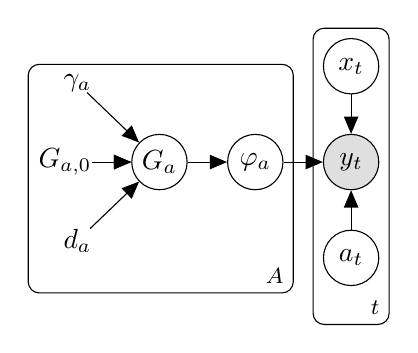
\begin{tikzpicture}
	% Nodes
	% Return y
	\node[obs] (y-t) {$y_{t}$};
	% Action a
	\node[latent, below=0.5 of y-t] (a-t) {$a_t$};
	% Context x
	\node[latent, above=0.5 of y-t]  (x-t) {$x_t$};
	% Nonparametric parameters
	\node[latent, left=0.5 of y-t, xshift=0cm] (varphi-a) {$\varphi_{a}$};
	% Nonparametric distribution
	\node[latent, left=0.5 of varphi-a, xshift=0cm] (G-a) {$G_{a}$};
	
	% Hyperparameters
	\node[const, left=0.5 of G-a, yshift=-1.0cm] (d-a) {$d_{a}$} ;
	\node[const, left=0.5 of G-a, yshift=0.0cm]  (G-a0) {$G_{a,0}$} ;
	\node[const, left=0.5 of G-a, yshift=1.0cm] (gamma-a) {$\gamma_{a}$} ;
	
	% Edges
	% Hyperparameters to distribution
	\edge {gamma-a,G-a0} {G-a} ;
	\edge {d-a,G-a0} {G-a} ;
	% Connect distribution to parameters
	\edge {G-a} {varphi-a} ;
	% Connect parameters, context and arm to observation
	\edge {varphi-a,x-t,a-t} {y-t} ;
	
	% Plates
	% Over time
	\plate {t} {(a-t)(x-t)(y-t)} {$t$} ;
	% Over each arm
	\plate {a}{
		(d-a)(gamma-a)(G-a0) % hyperparameters
		(G-a) % distribution
		(varphi-a) % parameters
	} {$A$} ;
\end{tikzpicture}
		}
		\vspace*{-1ex}
		\caption{The Bayesian nonparametric mixture bandit distribution.}
		\label{fig:pgm_nonparametric_bandit}
	\end{center}
	\vspace*{-4ex}
\end{figure}

By allowing each arm of the bandit to draw from a different nonparametric model, we have full flexibility to estimate each per-arm distribution independently, covering MAB cases with distinct reward model classes per-arm. This setting is a very powerful extension of the MAB problem, which has not attracted interest so far.\footnote{An alternative would be to consider a hierarchical nonparametric model~\cite{j-Teh2006,j-Teh2010}, where all arms are assumed to obey the same family of distributions, but only their mixture proportions vary across arms. We provide details of this alternative model in Section~\ref{asec:nonparametric_hierarchical_mixture_model} of the Appendix.}

In this work, we model context-conditional complex reward densities with nonparametric Gaussian mixture models per-arm,
\begin{equation}
y_{t} \sim p(Y|a,x_t,\varphi) = \sum_{k=1}^{K_a} \frac{n_{a,k}-d_a}{n_a+\gamma_a} \cdot \N{Y|x_{t}^\top w_{a,k}, \sigma_{a,k}^2} + \frac{\gamma_a+K_ad_a}{n_a+\gamma_a} \N{Y|x_{t}^\top w_{a,k_{new}}, \sigma_{a,k_{new}}^2} \;.
\label{eq:nonparametric_Gaussian_mixture}
\end{equation}
Each per-arm distribution is modeled independently, \ie $d_a$, $\gamma_a$, $\varphi_{a,k}=\{w_{a,k}, \sigma_{a,k}^2 \}$, and the number of mixtures $K_a$, are per-arm specific parameterizations. Each per-arm and per-mixture emission distribution is a context-conditional Gaussian density
\begin{equation}
p(Y|a,k,x,\varphi_{a,k})=\N{Y|x^\top w_{a,k}, \sigma_{a,k}^2} \;,
\end{equation}
with an expectation that is linearly dependent on the context at time $t$, $\mu_{t,a,k}=x_t^\top w_{a,k}$. The conjugate prior of each of the mixands is a Normal-inverse Gamma
\begin{equation}
G_{a,0}(\varphi_a) = \NIG{w_a, \sigma_a^2 |u_{a,0}, V_{a,0},\alpha_{a,0}, \beta_{a,0}} \;,
\end{equation}
with hyperparameters $\varPhi_{a,0}=\{u_{a,0}, V_{a,0},\alpha_{a,0}, \beta_{a,0}\}$.

Eqn.~\eqref{eq:nonparametric_Gaussian_mixture} describes per-arm nonparametric Gaussian mixture densities, with a Pitman-Yor nonparametric prior as described in Eqn.~\eqref{eq:pitman_yor_mixture}. With this proposed per-arm nonparametric mixture of Gaussian densities, we make a very flexible reward model assumption that automatically adjusts to the observed data: we are nonparametrically estimating per-arm complex reward densities.
The Bayesian nonparametric literature has already established strong convergence results on the density estimation properties of these models: for a wide class of continuous distributions, the nonparametric posterior converges to the true data-generating density, under mild regularity conditions~\cite{j-Ghosal1999, j-Lijoi2004, j-Tokdar2006, j-Ghosal2007, j-Bhattacharya2010, j-Pati2013}.
 
At every interaction of the MAB with the world, rewards $y_t$ are \iid drawn from a context dependent unknown distribution of the played arm $y_{t}\sim P(Y|a,x,\thetastar)$, which we here approximate via Bayesian nonparametric mixture models. The reward model class we consider here is a very flexible one, which adjusts its complexity as data are observed~\cite{b-Ghosal2017}.
After observing rewards $y_{1:n}$, and conditioned on the auxiliary assignment variables $z_{1:n}$, the posteriors of per-arm and mixture parameters $\varphi_{a,k}$ follow a Normal-inverse Gamma distribution, $G_{a,n_{a,k}}(\varphi_{a,k})=\NIG{w_{a,k}, \sigma_{a,k}^2 |\varPhi_{a,k,n_{a,k}}}$, with updated hyperparameters $\varPhi_{a,k,n_{a,k}}$ that depend on the number $n_{a,k}$ of rewards observed after playing arm $a$ that are assigned to mixture $k$. That is, $\varPhi_{a,k,n_{a,k}}=\{u_{a,k,n_{a,k}}, V_{a,k,n_{a,k}},\alpha_{a,k,n_{a,k}}, \beta_{a,k,n_{a,k}} \}$ with
\begin{equation}
\hspace*{-1ex}\begin{cases}
V_{a,k,n_{a,k}}^{-1} = x_{1:n} R_{a,k} x_{1:n}^\top + V_{a,0}^{-1} \;,\\
u_{a,k,n_{a,k}}= V_{a,k,n_{a,k}} \left( x_{1:n} R_{a,k} y_{1:n} + V_{a,0}^{-1} u_{a,0}\right) \;, \\
\alpha_{a,k,n_{a,k}} = \alpha_{a,0} + \frac{1}{2} \tr{R_{a,k}} \;, \\
\beta_{a,k,n_{a,k}} = \beta_{a,0} + \frac{1}{2}\left(y_{1:n}^\top R_{a,k}y_{1:n} \right) + \frac{1}{2}\left( u_{a,0}^\top V_{a,0}^{-1} u_{a,0} - u_{a,k,n_{a,k}}^\top V_{a,k,n_{a,k}}^{-1} u_{a,k,n_{a,k}} \right) \; ,
\end{cases}
\label{eq:posterior_hyperparameters}
\end{equation}
where $R_{a,k}\in\Real^{n_a\times n_a}$ is a sparse diagonal matrix with elements $\left[R_{a,k}\right]_{n,n^\prime}=\mathds{1}[a_n=a,z_n=k]$, and $n_{a}=\sum_{k=1}^{K_a} n_{a,k}$, the number of rewards observed after playing arm $a$. The number of mixtures per-arm $K_a$ of the bandit is independently drawn from its own Pitman-Yor process. Note that the above expression can be computed sequentially as data are observed for the played arm.

The predictive emission distribution after marginalization of the parameters $\varphi_{a,k}$, needed for solving Eqn.~\eqref{eq:gibbs_mixture_assignment}, follows a conditional Student-t distribution
\begin{equation}
p_{a,k}(Y|a,x,\varPhi_{a,k}) = \T{Y|\nu_{a,k,y}, m_{a,k,y}, r_{a,k,y}}, \; \text{ with }
\begin{cases}
\nu_{a,k,y}=2\alpha_{a,k} \;, \\
m_{a,k,y} = x^\top u_{a,k} \;, \\
r_{a,k,y}^2 = \frac{\beta_{a,k}}{\alpha_{a,k}} (1+x^\top V_{a,k} x) \; .
\end{cases}
\label{eq:predictive_emission_univariate}
\end{equation}
The hyperparameters $\varPhi_{a,k}$ above are those of the prior $\varPhi_{a,0}$, or the posterior $\varPhi_{a,k,n_{a,k}}$, depending on whether the predictive density refers to a new mixture $k_{new}$, or a `\textit{seen}' mixture $k$, for which $n_{a,k}$ observations have been already assigned to, respectively.

Similarly, the likelihood of a set of rewards assigned to a per-arm mixture $k$, $Y_{a,k}=y_{1:n}\cdot \mathds{1}[a_n=a,z_n=k]$, given their associated contexts $X_{a,k}=x_{1:n} \cdot \mathds{1}[a_n=a,z_n=k]$, follows the matrix t-distribution
\begin{equation}
\begin{split}
& p(Y_{a,k}|X_{a,k},X_{\backslash a,k},Y_{\backslash a,k},\varPhi_{a,k}) = \MT{Y_{a,k}|\nu_{Y_{a,k}}, M_{Y_{a,k}}, \Psi_{Y_{a,k}}, \Omega_{Y_{a,k}}} \; , \\
& \text{ with }
\begin{cases}
\nu_{Y_{a,k}}=2 \alpha_{a,k} \;, \\
M_{Y_{a,k}}= X_{a,k}^\top u_{a,k} \;, \\
\Psi_{Y_{a,k}} = I_{n_{a,k}} + X_{a,k}^\top V_{a,k} X_{n_{a,k}} \;, \\
\Omega_{Y_{a,k}} = 2 \beta_{a,k} \; .
\end{cases}
\end{split}
\label{eq:predictive_emission_multivariate}
\end{equation}

\subsection{Nonparametric Gaussian mixture model Thompson sampling}
\label{ssec:nonparametric_thompson_sampling}

We leverage the nonparametric Gaussian mixture model described above, and combine it with a posterior sampling MAB policy, \ie Thompson sampling~\cite{j-Russo2018}. The proposed Thompson sampling for contextual bandits with nonparametric Gaussian mixture reward models is presented in Algorithm~\ref{alg:nonparametric_ts}. At each interaction with the world, Thompson sampling decides which arm to play next based on a random parameter sample, drawn from the posterior distribution updated with all the information available at time $t$.

For nonparametric models as in Eqn~\eqref{eq:nonparametric_Gaussian_mixture}, one draws per-arm and per-mixture Gaussian parameters $\varphi_{a,k}$ from the posterior distributions with updated hyperparameters $\varPhi_{a,k,n_{a,k}}$ in Eqn.~\eqref{eq:posterior_hyperparameters}, conditioned on the mixture assignments $z_{1:n}$ determined by the Gibbs sampler in Eqn.~\eqref{eq:gibbs_mixture_assignment} with marginalized densities in Eqns.~\eqref{eq:predictive_emission_univariate} and~\eqref{eq:predictive_emission_multivariate}. Given the inferred sufficient statistics of the assignments (\ie the counts $n_{a,k}$ of rewards observed for arm $a$ and assigned to mixture $k$), and the drawn posterior parameter samples $w_{a,k}^{(t+1)}$, one computes the expected reward for each arm of the nonparametric bandit, \ie
\vspace*{-1ex}
\begin{equation}
\begin{split}
\mu_{t+1,a}(x_{t+1},\varphi_{a}^{(t+1)})&=\sum_{k=1}^{K_a} \frac{n_{a,k}-d_a}{n_a+\gamma_a} \cdot \left(x_{t+1}^\top w_{a,k}^{(t+1)}\right) + \frac{\gamma_a+K_ad_a}{n_a+\gamma_a} \cdot \left(x_{t+1}^\top w_{a,k}^{(t+1)} \right)\; .
\end{split}
\label{eq:nonparametric_expected_reward}
\end{equation}

\subsubsection{Regret bound}
\label{sssec:nonparametric_thompson_sampling_regret_bound}

In order to bound the regret of the proposed algorithm, we leverage asymptotic posterior converge rates, \ie the rate at which the distance between two densities becomes exponentially small as the number of observation grows.

A Thompson sampling based policy computes the probability of each arm being optimal, which is equivalent to the expectation of the optimal arm indicator function with respect to the joint posterior distribution of the expected rewards, \ie
\begin{equation}
\pi(a|x_{t},\HH_{1:t-1})=\Prob{a=\argmax_{a^\prime \in \A} \mu_{t,a^\prime}|p(\mu_t)} = \eValue{p(\mu_t)}{\myind{a=\argmax_{a^\prime \in \A}\mu_{t,a^\prime}|p(\mu_t)}} 
\end{equation}
The posterior $p(\mu_t)$ above is the joint distribution over the expected rewards of all arms: $\mu_{t}=\{\mu_{t,a}\}, \forall a\in \A$. This posterior is a multivariate distribution over all arms of the bandit, \ie of dimension $|\A|$. Note how the indicator function $\myind{a=\argmax_{a^\prime \in \A}\mu_{t,a^\prime}|p(\mu_t)}$ for each arm $a$ requires the posterior over all arms $a^\prime \in \A$ as input.

\begin{lemma}
	The difference in action probabilities between two Thompson sampling policies is bounded by the total-variation between the posterior distributions of their expected rewards, \ie $p(\mu_{t}|h_{1:t})$ and $q(\mu_{t}|h_{1:t})$, respectively,
	\begin{equation}
	\pi(a|p) - \pi(a|q) = \eValue{p}{\myind{a=\argmax_{a^\prime \in \A} \mu_{t,a^\prime}|p}} - \eValue{q}{\myind{a=\argmax_{a^\prime \in \A} \mu_{t,a^\prime}|q}} \leq \delta_{TV}(p,q)
	\nonumber
	\end{equation}
	\label{lemma:total_variation_bounds_diff_policies}
\end{lemma}

We make use of the above lemma to bound the cumulative regret of the proposed Thompson sampling with Dirichlet process mixtures (\ie $d_a=0, \forall a$) of Gaussian distributions, for bandits with true reward densities that meet certain regularity conditions.

\begin{theorem}
	The regret of a Dirichlet process Gaussian mixture model based Thompson sampling algorithm is bounded by
	\begin{equation}
	R_T	=\eValue{}{\sum_{t=1}^T y_{t,\astar_t}-y_{t,a_t} } \leq 2 C_A A \sqrt{T} (C_p + C_{\ptilde} (\log T)^\kappa ) = O(A \log^\kappa T \sqrt{T}) \; ,
	\nonumber
	\end{equation}
	where the expectations are taken over the unknown rewards, the random actions of the stochastic policies, and the true $\pstar$ reward models that meet mild regularity conditions. 
	\label{th:regret_bound}
\end{theorem}
The proofs of Lemma~\ref{lemma:total_variation_bounds_diff_policies} and Theorem~\ref{th:regret_bound} are provided in Section \ref{asec:nonparametric_thompson_sampling_regret_bound} of the Appendix. The proof of Theorem~\ref{th:regret_bound} results from bounding the regret introduced by two factors: the first, related to the use of Thompson sampling (\ie a policy that does not know the true parameters of the reward distribution, but has knowledge of the true model class); and the second, that accounts for the convergence of the posterior of a nonparametric model to that of the true data generating distribution. The logarithmic term $\log^\kappa T$ in the bound appears due to the convergence rate of the nonparametric density estimation, where the exponent $\kappa\geq 0$ depends on the tail behavior of the base measure and the associated priors of the Dirichlet process --- see Section \ref{asec:nonparametric_thompson_sampling_regret_bound} of the Appendix and posterior convergence analysis in~\cite{j-Ghosal2001,j-Ghosal2007}.

%Nonparametric TS
%\vspace*{-3ex}
\begin{algorithm}
	\caption{Nonparametric Gaussian mixture model based Thompson sampling}
	\label{alg:nonparametric_ts}
	\begin{algorithmic}[1]
		\STATE {\bfseries Input:} Number of arms $A$
		\STATE {\bfseries Input:} Per-arm model hyperparameters $d_a$, $\gamma_a$, $\varPhi_{a,0}$
		\STATE {\bfseries Input:} Gibbs convergence criteria $\epsilon$ and $Gibbs_{max}$ 
		\STATE $\HH_1=\emptyset$
		\FOR{$t=1, \cdots, T$}
		\STATE Receive context $x_{t+1}$
		\FOR{$a=1, \cdots, A$}
		\STATE Draw parameters from the posterior $\varphi_{a,k}^{(t+1)} \sim G_{a,k,n_{a,k}}(\varPhi_{a,k}), \forall k$, as in Eqn.~\eqref{eq:posterior_hyperparameters}
		\STATE Compute $\mu_{t+1,a}(x_{t+1},\varphi_{a}^{(t+1)})$ as in Eqn.~\eqref{eq:nonparametric_expected_reward}
		\ENDFOR
		\STATE Play arm $\; a_{t+1}=\argmax_{a^\prime \in \A} \mu_{t+1,a^\prime}(x_{t+1},\varphi_{a^\prime}^{(t+1)})$
		\STATE Observe reward $y_{t+1}$
		\STATE $\HH_{1:t+1}=\HH_{1:t} \cup \left\{x_{t+1}, a_{t+1}, y_{t+1}\right\}$
		\WHILE{NOT Gibbs convergence criteria}
		\STATE Update mixture assignments $z_{1:n}$ based on Eqn.~\eqref{eq:gibbs_mixture_assignment}
		\STATE Compute sufficient statistics $n_{a,k}$
		\STATE Update parameter posteriors $\varPhi_{a,k,n_{a,k}}$ based on Eqn.~\eqref{eq:posterior_hyperparameters}
		\ENDWHILE
		\ENDFOR
	\end{algorithmic}
\end{algorithm}

\subsubsection{Computational complexity}
\label{sssec:nonparametric_thompson_sampling_computational_complexity}
The Gibbs sampler in lines 14-18 within Algorithm~\ref{alg:nonparametric_ts} is run $Gibbs_{steps}$ until a stopping criteria is met: either the model likelihood of the sampled chain is stable within an $\epsilon$ margin between steps, or a maximum number of iterations $Gibbs_{max}$ is reached. As new rewards $y_{t+1,a_{t+1}}$ are acquired, updates to assignments $z_{t^\prime,a_{t+1}}$ are done sequentially within the Gibbs sampler for $t^\prime=\{1,\cdots,t+1 | a_{t^\prime}=a_{t+1}\}$ --- only the posterior over the last played armed $a_{t+1}$ is recomputed. Since Eqn.~\eqref{eq:posterior_hyperparameters} can be sequentially computed for each per-arm observation, the computational cost of the Gibbs sampler grows with the number of available observation of the played arm. The overall computational cost is $O(T \cdot Gibbs_{steps})$ per-interaction with the world, \ie per newly observed reward $y_{t+1,a_{t+1}}$.

\vspace*{-2ex}
\paragraph{Practical recommendation:} In general, one should run the Gibbs sampler to full convergence, \ie until the $\epsilon$ likelihood margin is met --- recommended when no computational constraints are in place. However, due to the sequential acquisition of observations in the bandit setting, and the need to only update the posterior for the played arm, the Gibbs sampler is warm-started at each interaction with the world, and good convergence can be achieved in few iterations. The Gibbs sampler is run from a good starting point: the per-arm parameter space that describes all but this newly observed reward $y_{t+1,a_{t+1}}$. In practice, and because of the warm-start, one can limit the number of Gibbs sampler iterations per-MAB interaction to upper-bound the algorithm's complexity to $O(T\cdot Gibbs_{max})$, yet achieve satisfactory performance. We emphasize that we do consider a Gibbs sampler that runs until full convergence, but propose to limit the number of Gibbs iterations as an empirical recommendation with good regret performance, yet upper-bounded computational complexity of $O(T \cdot Gibbs_{max})$ per MAB interaction with the environment.

\section{Evaluation}
\label{sec:evaluation}

We evaluate the performance of the proposed nonparametric mixture model based Thompson sampling in diverse synthetic and realistic datasets.

Results for different parameterizations of contextual linear Gaussian MAB settings (provided in Section~\ref{asec:evaluation_linearGaussian} of the Appendix) show that the proposed method attains same cumulative regret than the Thompson sampling in~\cite{j-Agrawal2012}, which correctly assumes the true underlying contextual linear Gaussian model, and can compute posterior updates in closed form. That is, the proposed nonparametric Thompson sampling method is as good as the analytical alternative: the per-arm posterior densities quickly converge to the true unknown distribution, incurring in no additional regret.

We here focus on more challenging MABs, \ie those where the underlying reward distributions do not fit into the exponential family assumption. The following studied scenarios differ in the amount of mixture overlap and the similarity between arms:
\begin{equation}
\texttt{Scenario A:}\\
\resizebox{0.7\textwidth}{!}{$
\begin{cases}
p_{0}(y|x_t,\theta) = 0.5 \cdot \N{y|x_t^\top (1 \; 1), 1} + 0.5 \cdot \N{y|x_t^\top (2 \; 2), 1}\\
p_{1}(y|x_t,\theta) = 0.3 \cdot \N{y|x_t^\top (0 \; 0), 1} + 0.7 \cdot \N{y|x_t^\top (3 \; 3), 1}
\end{cases}
$}
\nonumber
\end{equation}
\vspace*{-2ex}
\begin{equation}
\texttt{Scenario B:}\\
\resizebox{0.85\textwidth}{!}{$
\begin{cases}
p_{0}(y|x_t,\theta) = \N{y|x_t^\top (1 \; 1), 1}\; ,\\
p_{1}(y|x_t,\theta) = 0.5 \cdot \N{y|x_t^\top (1 \; 1), 1} + 0.5 \cdot \N{y|x_t^\top (2 \; 2), 1}\\
p_{2}(y|x_t,\theta) = 0.3 \cdot \N{y|x_t^\top (0 \; 0), 1} + 0.6 \cdot \N{y|x_t^\top (3 \; 3), 1} + 0.1 \cdot \N{y|x_t^\top (4 \; 4), 1} 
\end{cases}
$}
\nonumber
\end{equation}
%\vspace*{-1ex}
\begin{equation}
\texttt{Scenario C:}\\
\resizebox{0.7\textwidth}{!}{$
\begin{cases}
p_{0}(y|x_t,\theta) = 0.75 \cdot \N{y|x_t^\top (0 \; 0), 1} + 0.25 \cdot \N{y|x_t^\top (0 \; 0), 10} \\
p_{1}(y|x_t,\theta) = 0.75 \cdot \N{y|x_t^\top (2 \; 2), 1} + 0.25 \cdot \N{y|x_t^\top (2 \; 2), 10}
\end{cases}
$}
\nonumber
\end{equation}

The reward distributions of these contextual bandits are Gaussian mixtures dependent on a two dimensional uncorrelated uniform context, \ie $x_{i,t}\sim\U{0,1}$, $i\in\{0,1\}$, $t\in \Natural$. These reward distributions are complex --- not within the exponential family of distributions: they are all multi-modal, unbalanced in \texttt{Scenarios A} and \texttt{B}, and with heavy tails in \texttt{Scenario C}. In \texttt{Scenario A}, there is a significant overlap between arm rewards, with quite unbalanced mixtures for arm 1. \texttt{Scenario B} describes a MAB with different per-arm reward distributions: a linear Gaussian distribution for arm 0, a bi-modal Gaussian mixture for arm 1, and an unbalanced Gaussian mixture with three components for arm 2. Finally, \texttt{Scenario C} models heavy-tailed distributions, where the bandit is subject to outlier rewards.

We recall that, even if each scenario is a different MAB setting --- with diverse model classes per-arm in \texttt{Scenario B} --- our proposed Thompson sampling framework is readily applicable to all. On the contrary, alternative methods, such as those based on Gaussian processes~\cite{ip-Srinivas2010,ip-Gruenewaelder2010,ic-Krause2011} require the specification of the correct model class of the MAB they are targeting. These methods, although interesting and flexible, require knowledge of the true underlying model class (\ie what mean and kernel functions to use) and suffer from model misspecification. 

Here, since there is no alternative algorithm to address all MAB scenarios jointly, we compare our proposed Algorithm~\ref{alg:nonparametric_ts} to an Oracle Thompson sampling: one that knows the true number of underlying mixtures of the problem it is targeted to. Note that this is only possible in simulation, where we have access to the reward generation function. Specifically, each Oracle Thompson sampling uses a Dirichlet distribution with the true underlying dimensionality $K$ per-scenario --- instead of a nonparametric prior on the mixtures --- and follows the Gibbs sampler as explained in Section~\ref{sec:proposed_method}.

For each considered scenario, we compare the performance of our proposed method to that of each per-scenario tuned Oracle Thompson sampling. We reiterate that this is only possible in a simulated environment, as knowing the reward complexity of a MAB beforehand is impractical --- an alternative would be to run multiple model assumptions in parallel, with a subsequent model selection.

Fig.~\ref{fig:linear_gaussian_mixtures} shows the cumulative regret --- as in Eqn.~\eqref{eq:cumulative_regret} --- of the proposed nonparametric mixture model Thompson sampling, along with each per-scenario Oracle Thompson sampling. Due to the capacity of Bayesian nonparametrics to autonomously adjust the complexity of the model to the sequentially observed data, the proposed method can, without any per-scenario tuning  ($d_a=0$ and $\gamma_a=0.1$, $\forall a$, in all the experiments), readily target all of them. 

\begin{figure}[!h]
	\centering
	\begin{subfigure}[c]{0.49\textwidth}
		\vspace*{-2ex}
		\includegraphics[width=\textwidth]{./figs/linearGaussianMixture/hard/cumregret_R3629}
		\vspace*{-4ex}
		\caption{\texttt{Scenario A}.}
		\label{fig:linear_gaussian_mixture_hard}
	\end{subfigure}
	\begin{subfigure}[c]{0.49\textwidth}
		\vspace*{-2ex}
		\includegraphics[width=\textwidth]{./figs/linearGaussianMixture/unbalanced/cumregret_R3641}
		\vspace*{-4ex}
		\caption{\texttt{Scenario B}.}
		\label{fig:linear_gaussian_mixture_unbalanced}
	\end{subfigure}

	\begin{subfigure}[c]{0.49\textwidth}
		\includegraphics[width=\textwidth]{./figs/linearGaussianMixture/heavy/cumregret_R3250}
		\vspace*{-4ex}
		\caption{\texttt{Scenario C}.}
		\label{fig:linear_gaussian_mixture_heavy}
	\end{subfigure}
	\begin{subfigure}[c]{0.49\textwidth}
		\includegraphics[width=\textwidth]{./figs/linearGaussianMixture/heavy/cumregret_R3250_mispecified}
		\vspace*{-4ex}
		\caption{\texttt{Scenario C}, with a mispecified model.}
		\label{fig:linear_gaussian_mixture_mispecified}
	\end{subfigure}
	\vspace*{-1ex}
	\caption{Mean regret (standard deviation shown as shaded region) for at least 1000 independent realizations of the presented methods in all scenarios.}
	\label{fig:linear_gaussian_mixtures}
\vspace*{-1ex}
\end{figure}

Our proposed method not only fits the underlying reward function accurately in all cases, but attains reduced regret as well: \%13 and \%19 cumulative regret reduction at $t=500$ for Scenario A and B, respectively. This is achieved in the most challenging (not in the exponential family) MAB settings: \ie unbalanced and heavy tailed bandit distributions, for bandits with different per-arm distributions, and when compared to a per-scenario Oracle Thompson sampling policy (\ie one that knows the true underlying complexity of the model).
We further highlight the built-in flexibility of the nonparametric method by showing in Fig.~\ref{fig:linear_gaussian_mixture_mispecified} how Thompson sampling with a mispecified model (\ie fitting a unimodal distribution to the heavy-tailed \texttt{Scenario B}) suffers in comparison to the proposed nonparametric method (a \%18 cumulative regret reduction is attained).

The proposed nonparametric generative modeling provides further per-arm reward understanding (by plotting or computing other figures of merit from these distributions), as the learned per-arm posteriors converge to the true posteriors. We note that posterior density convergence does not imply that it is consistent in $K$ --- that is, on data from a finite mixture, nonparametrics do not necessarily concentrate at the true number of components~\cite{j-Miller2014}. However, the goal of the Thompson sampling is to approximate the posterior distribution accurately enough to compute its expected value and draw samples from it, in order to maximize the cumulative expected reward, which the results above show is attained.

Regarding convergence of the Gibbs sampler, we argue in Section~\ref{sssec:nonparametric_thompson_sampling_computational_complexity} that due to the \textit{warm-start} at each interaction with the world, good convergence can be achieved in few iterations. That is, Gibbs sampling inference aligns well with the online nature of bandits, as the sampler is updated only with the reward observed for the last played arm. Because of this incremental availability of observations, the sampler achieves quick convergence (in our experiments, a 1\% log-likelihood relative difference between iterations was usually achieved within 5-10 iterations).

We show in Figure~\ref{fig:cumregret_gibbs} that no significant regret performance improvement is achieved by letting the sampler run for a higher number of iterations. \textit{A good enough} posterior convergence at a limited computational budget is possible because the Gibbs sampler is run, at each interaction with the world, from a good starting point: the per-arm parameter space that describes all but this newly observed reward --- $Gibbs_{max}$ updates over all $t_a$ observations for the played arm are still computed.
Therefore, when computational constraints are appropriate (\eg for real time bandits) limiting the number of Gibbs iterations can still achieve satisfactory cumulative regret.

\begin{figure}[!h]
	\centering
	\includegraphics[width=0.5\textwidth]{./figs/linearGaussianMixture/unbalanced/cumregret_gibbs}
	\caption{Cumulative regret on Scenario B, for different maximum number of Gibbs iterations.}
	\label{fig:cumregret_gibbs}
\vspace*{-1ex}
\end{figure}

We finally evaluate the proposed method in a real application as well, \ie the recommendation of personalized news articles, in a similar fashion as done by~\citet{ic-Chapelle2011}. We picked $A=20$ articles shown during two days in the \textit{Today Module of the Yahoo! Front Page}.
The goal is to choose the most interesting article for each user, by counting the total number of clicks. We evaluated both the proposed nonparametric Gaussian mixture model, and the logistic reward model as proposed in~\cite{ic-Chapelle2011,ic-Dumitrascu2018}. All details about the dataset and the implemented MAB models are provided in Section~\ref{asec:evaluation_yahoo} of the Appendix. We observe in Table~\ref{tab:yahoo_logistic_crt} that the proposed method as in Algorithm~\ref{alg:nonparametric_ts} is able to attain satisfactory averaged CTR in both 20-armed MAB scenarios, without any specific modeling or parameter assumptions.

% CTR table
%%%%%%%%%%%%%%%%%%%%%%%%
%% Table for yahoo data with logistic bandits
%%%%%%%%%%%%%%%%%%%%%%%%
\begin{table}[!ht]
	\begin{center}
		\resizebox*{\textwidth}{!}{
			\begin{tabular}{*{3}{|c}|}
				\hline
				% Header
				Model \cellcolor[gray]{0.6} & CTR\cellcolor[gray]{0.6} & Normalized CTR\cellcolor[gray]{0.6} \\ \hline
				% table starts
				\cellcolor[gray]{0.8} Logistic rewards, static arms & 0.0670 +/- 0.0088 & 1.6095 +/- 0.2115  \\ \hline
				\cellcolor[gray]{0.8} Logistic rewards, time-evolving arms & 0.0655 +/- 0.0082 & 1.5745 +/- 0.2064 \\ \hline
			\end{tabular}
		}
		\caption{CTR results for SMC-based policies on the news article recommendation dataset.
			The normalized CTR is with respect to a random recommendation baseline.}
		\label{tab:yahoo_logistic_crt}
	\end{center}
	\vspace*{-2ex}
\end{table}


We conclude by reiterating that the proposed nonparametric Thompson sampling avoids stringent case-by-case model assumptions, and does not require any parameter tuning for each specific MAB, yet attains competitive regret when faced with distinct MAB reward distributions: the same algorithm is run for contextual Gaussian, logistic, and other complex (not in the exponential family) multi-armed bandits.

\section{Conclusion}
\label{sec:conclusion}

We contribute to the field of sequential decision processes by proposing a nonparametric mixture model based Thompson sampling. We merge the advances in the field of Bayesian nonparametrics with a state of the art MAB policy (\ie Thompson sampling), and allow its extension to complex domains with model uncertainty. The proposed Bayesian algorithm provides flexible modeling of convoluted reward functions with convergence guarantees, and attains the exploration-exploitation trade-off in complex MABs with minimal assumptions. Empirical results show good cumulative regret performance of the proposed nonparametric Thompson sampling in challenging domains, remarkably adjusting to the complexity of the underlying bandit --- and bypassing model mispecification --- in an online fashion. With the ability to sequentially learn the nonparametric mixture model that best approximates the true reward distribution, the proposed method can be applied to diverse MAB settings (without stringent model specifications) and attain reduced regret. A future direction is to tighten the presented regret bound, as well as to apply the proposed method to other real MAB applications where complex models are likely to outperform simpler ones.

%%%%%%%%%%%%%%%%%%%%%%%%%%%%%%%%%%%%%%%%%%%%%%%%%%%%%%%%%%%%%%%%%%%%%%%%%%%%%%%
% Acknowledgements 
%\section*{Acknowledgements}
%%%%%%%%%%%%%%%%%%%%%%%%%%%%%%%%%%%%%%%%%%%%%%%%%%%%%%%%%%%%%%%%%%%%%%%%%%%%%%%

%%%%%%%%%%%%%%%%%%%%%%%%%%%%%%%%%%%%%%%%%%%%%%%%%%%%%%%%%%%%%%%%%%%%%%%%%%%%%%%
%%% References
% Generate bibliography from the specified bibliography file
%\bibliography{../literature}
% After compiling, include bbl for ArXiv
\documentclass{article}

%%%%%%%%%%%%%%%%%%%%%%%% STYLE INFO %%%%%%%%%%%%%%%%%%%%%%%%
\usepackage[margin=1.5in]{geometry}

%%%%%%%%%%%%%%%%%%%%%%%% IMPORTS %%%%%%%%%%%%%%%%%%%%%%%%
%%%% PACKAGES TO USE
\usepackage[utf8]{inputenc} % allow utf-8 input
\usepackage[T1]{fontenc}    % use 8-bit T1 fonts
\usepackage{hyperref}       % hyperlinks
\usepackage{url}            % simple URL typesetting
\usepackage{booktabs}       % professional-quality tables
\usepackage{amsfonts}       % blackboard math symbols
\usepackage{nicefrac}       % compact symbols for 1/2, etc.
\usepackage{microtype}      % microtypography
\usepackage{enumerate}
% Math related
\usepackage{amsmath}
\usepackage{amsthm} % For proof environment
\usepackage{mathtools}
% Indicator
%\usepackage{bbm} %uses Type3
\usepackage{dsfont} %works with Type1
% Figures and subfigures
\usepackage{graphicx}
\usepackage{caption}
\usepackage{subcaption}
\usepackage{float} %Stay where told
% Tables
\usepackage{booktabs} % for professional tables
\usepackage{multirow} % to be able to have multiple row expanding cell
\usepackage[table]{xcolor}

% Algorithms
\usepackage{algorithm}
\usepackage{algorithmic}
% To draw graphs
\usepackage{tikz}
\usetikzlibrary{bayesnet} % Library for bayesian networks

% Lemmas, Theorems and proofs
\newtheorem{theorem}{Theorem}
\newtheorem{lemma}{Lemma}
% Bibliography
%\usepackage[round,numbers,sort]{natbib} % Round parentheses for references ()
\usepackage[numbers,sort]{natbib} % Square parentheses for references []
% Select a .bst file for the style
\bibliographystyle{abbrvnat}
% Reference column balancing
\usepackage{flushend}

%%%% DEFINITIONS-MACROS
% Real line
\def \Real{{\mathbb R}} 
\def \Natural{{\mathbb N}} 
%Expected value
\newcommand{\eValue}[2]{\mathbb{E}_{#1}\left\{ #2 \right\}}
\newcommand{\Prob}[1]{\mathbb{P}\left( #1 \right)}
% Kullback-Leibler
\newcommand{\KL}[2]{\mathrm{KL}\left( #1 \| #2\right)}
% My small matrix
\newcommand{\mySmallMatrix}[1]{\left(\begin{smallmatrix} #1 \end{smallmatrix}\right)}
%Determinant
\newcommand{\mydet}[1]{\left| #1 \right|}
% My indicator function
\newcommand{\myind}[1]{\ind{}\left[#1\right]}
% d in integral
\newcommand{\dd}[1]{\mathrm{d} #1}
% TK
\newcommand{\TK}[1]{\textcolor{red}{TK: #1}}

% Useful in Bandits
\newcommand{\A}{\mathcal{A}}
\newcommand{\Astar}{A^*}
\newcommand{\astar}{a^*}
\newcommand{\pstar}{p^*}
\newcommand{\pistar}{\pi^*}
\newcommand{\Atilde}{\tilde{A}}
\newcommand{\atilde}{\tilde{a}}
\newcommand{\ptilde}{\tilde{p}}
\newcommand{\pitilde}{\tilde{\pi}}
\newcommand{\thetastar}{\theta^*}
\newcommand{\thetatilde}{\tilde{\theta}}
\newcommand{\Y}{\mathcal{Y}}
\newcommand{\HH}{\mathcal{H}}

% Abbreviations
\newcommand{\iid}{i.i.d. }
\newcommand{\ie}{i.e., }
\newcommand{\Ie}{I.e., }
\newcommand{\eg}{e.g., }
\newcommand{\Eg}{E.g., }
\newcommand{\etAl}{et al.\xspace}

%Distributions
\newcommand{\N}[1]{\mathcal{N}\left( #1\right)}
\newcommand{\MN}[1]{\mathcal{MN}\left( #1\right)}
\newcommand{\T}[1]{\mathcal{T}\left( #1\right)}
\newcommand{\MT}[1]{\mathcal{MT}\left( #1\right)}
\newcommand{\Dir}[1]{{\rm Dir\left( #1\right)}}
\newcommand{\Mult}[1]{{\rm Mult}\left( #1\right)}
\newcommand{\Cat}[1]{{\rm Cat}\left( #1\right)}
\newcommand{\Bin}[1]{{\rm Bin}\left( #1\right)}
\newcommand{\IG}[1]{{\rm IG}\left( #1\right)}
\newcommand{\NIG}[1]{{\rm NIG}\left( #1\right)}
\newcommand{\NIX}[1]{{\rm NIX}\left( #1\right)}
\newcommand{\IW}[1]{{\rm IW}\left( #1\right)}
\newcommand{\NIW}[1]{{\rm NIW}\left( #1\right)}
\newcommand{\Beta}[1]{{\rm Beta}\left( #1\right)}
\newcommand{\Ber}[1]{{\rm Ber}\left( #1\right)}
\newcommand{\U}[1]{\mathcal{U}\left( #1\right)}

%Others
\newcommand{\eqd}{\stackrel{d}{=}} % equal in distribution/law/measure
\newcommand{\abs}[1]{|{#1}|}
\newcommand{\argmax}{\mathop{\mathrm{argmax}}}
\newcommand{\argmin}{\mathop{\mathrm{argmin}}}
\newcommand{\var}{\textrm{Var}}
\newcommand{\cov}{\textrm{Cov}}
\newcommand{\Var}{\mathbb{V}\mathrm{ar}}
\newcommand{\Cov}{\mathrm{Cov}}
\newcommand{\tr}[1]{\mathrm{tr}\left\{ #1 \right\}} % trace
\newcommand{\diag}{\mathrm{diag}}
\newcommand{\ind}[1]{\mathds{1}_{#1}} % Indicator function
\newcommand{\kl}{\textrm{KL}}
\newcommand{\indep}{{\;\bot\!\!\!\!\!\!\bot\;}}
\newcommand{\eps}{\varepsilon}
%%%%%%%% end iurteaga %%%%%%%%
% Whether to add appendix or not
\def\addappendix{}

\title{Nonparametric Gaussian Mixture Models for the Multi-Armed Contextual Bandit}
\author{ I\~{n}igo Urteaga and Chris H.~Wiggins\\
	{\sf \{inigo.urteaga, chris.wiggins\}@columbia.edu} \\\\
	Department of	Applied Physics and Applied Mathematics\\
	Data Science Institute\\
	Columbia University\\
	New York City, NY 10027
}


\begin{document}

\maketitle

\begin{abstract}
We here adopt Bayesian nonparametric mixture models to extend multi-armed bandits in general, and Thompson sampling in particular, to complex scenarios where there is reward model uncertainty.
The multi-armed bandit is a sequential allocation task where an agent must learn a policy that maximizes long term payoff, where only the reward of the played arm is observed at each interaction with the world. In the stochastic bandit setting, at each interaction, the reward for the selected action is generated from an unknown distribution. Thompson sampling is a generative and interpretable multi-armed bandit algorithm that has been shown both to perform well in practice, and to enjoy optimality properties for certain reward functions. Nevertheless, Thompson sampling requires knowledge of the true reward model, for calculation of expected rewards and sampling from its parameter posterior. In this work, we extend Thompson sampling to complex scenarios where there is model uncertainty, by adopting a very flexible set of reward distributions: nonparametric Gaussian mixture models. The generative process of Bayesian nonparametric mixtures naturally aligns with the Bayesian modeling of multi-armed bandits: the nonparametric model autonomously determines its complexity in an online fashion, as new rewards are observed for the played arms. By characterizing each arm's reward distribution with independent Dirichlet process mixtures and per-mixture parameters, the proposed method sequentially learns the model that best approximates the true underlying reward distribution, achieving successful performance in synthetic and real datasets. Our contribution is valuable for practical scenarios, as it avoids stringent case-by-case model specifications, and yet attains reduced regret in diverse bandit settings.
\end{abstract}

\section{Introduction}
\label{sec:introduction}

%Recent advances in reinforcement learning~\cite{j-Gosavi2009} have sparked renewed interest in sequential decision making.
Sequential decision making aims to optimize interactions with the world (exploit), while simultaneously learning how the world operates (explore). Its origins can be traced back to the beginning of the past century, with important contributions within the field of statistics by~\citet{j-Thompson1935} and later~\citet{j-Robbins1952}.

The multi-armed bandit (MAB) is a natural abstraction for a wide variety of real-world challenges that require learning while simultaneously maximizing rewards~\cite{j-Lai1985, b-Lattimore2019}. The name `bandit' finds its origin in the playing strategy one must devise when facing a row of slot machines. The contextual MAB, where at each interaction with the world side information (known as `context') is available, is a natural extension of the bandit problem. Recently, a renaissance of the study of MAB algorithms has flourished~\cite{j-Agrawal2011,ip-Maillard2011}, and it has attracted interest from industry as well, due to its impact in digital advertising and products~\cite{j-Li2010, ic-Chapelle2011}. 

\citet{j-Thompson1933} sampling, also known as posterior sampling~\cite{j-Russo2014}, provides an elegant approach that tackles the exploration-exploitation dilemma in MABs. It updates a posterior over expected rewards for each arm, and chooses actions based on the probability that they are optimal. It has been empirically and theoretically proven to perform competitively for MAB models within the exponential family~\cite{ic-Chapelle2011,j-Agrawal2012,j-Agrawal2012a,ic-Korda2013}. Besides, its applicability to the more general reinforcement learning setting of Markov Decision Processes~\cite{j-Burnetas1997} has recently tracked momentum as well~\cite{ip-Gopalan2015,ic-Ouyang2017}.
Thompson sampling and the Bayesian approach to the MAB problem facilitate not only generative and interpretable modeling, but sequential and batch processing as well.
A Thompson sampling policy requires access to posterior samples of the model. Unfortunately, maintaining such posterior is intractable for distributions not in the exponential family~\cite{ic-Korda2013,j-Russo2018}.

Developing practical MAB methods to balance exploration and exploitation in complex domains remains largely unsolved.
In an effort to extend Thompson sampling to more complex scenarios, researchers have considered other flexible reward functions and Bayesian inference.
Recent approaches have embraced Bayesian neural networks and approximate inference for Thompson sampling. Variational methods, stochastic mini-batches, and Monte Carlo techniques have been studied for uncertainty estimation of reward posteriors~\cite{ip-Blundell2015, ic-Kingma2015, j-Lipton2016, ic-Osband2016, ip-Li2016}.

~\citet{ip-Riquelme2018} have recently benchmarked such techniques and reported that neural networks with approximate inference, even if successful for supervised learning, under-perform in the MAB setting. In particular,~\citet{ip-Riquelme2018} emphasize the issue of adapting the slow convergence uncertainty estimates of neural net based methods to MABs. In parallel, others have focused on extending Thompson sampling by targeting alternative classes of reward functions, such as approximating the unknown bandit reward functions with Gaussian mixture models~\cite{ip-Urteaga2018}.

Our contribution here is on exploiting Bayesian nonparametric mixture models for Thompson sampling to perform MAB optimization. Bayesian nonparametrics~\cite{j-Gershman2012} have been considered within the MAB setting for continuous action choices via Gaussian processes (GPs)~\cite{ip-Srinivas2010,ip-Gruenewaelder2010,ic-Krause2011}, or to allow for an unknown yet countable number of actions via hierarchical Pitman-Yor processes~\cite{j-Battiston2018}.

GPs are powerful nonparametric methods for modeling distributions over non-linear continuous functions~\cite{b-Rasmussen2005}, and have been used to model a continuum of MAB actions~\cite{ic-Krause2011}. Inference with GPs is computationally demanding --- it scales cubically in the number of observations --- limiting their applicability to the online setting, even if advancements such as pseudo-observations~\cite{ic-Snelson2006} or variational inference~\cite{ip-Titsias2009} can mitigate these shortcomings. 

Alternatively, \citet{j-Battiston2018} consider MABs with a discrete but unknown action space, and propose a hierarchical Pitman-Yor process for the unknown populations, with per-arm Bernoulli reward distributions. In this work, we are not interested in a nonparametric prior over arms (with specific per-arm reward distributions), but in sequential decision making with a discrete set of actions, for which there is uncertainty on the per-arm reward model.

We here propose to combine the flexibility of Bayesian nonparametrics with the large hypothesis space of mixture models, to address complex MABs.

In many contexts, a countably infinite mixture is a very realistic model to assume, and has been shown to succeed in modeling a diversity of phenomena~\cite{j-Gershman2012}. Nonparametric processes are useful priors for Bayesian density estimation. Within such framework, one uses nonparametric prior distributions over the mixing proportions, such as Dirichlet or Pitman-Yor processes~\cite{j-Teh2010}, which not only do not explicitly specify the number of mixtures, but allow for an unbounded number of mixtures to appear as data are observed. The important issue of nonparametric posterior consistency, with converge guarantees for a wide class of mixture models, has already been settled~\cite{j-Ghosal1999, j-Ghosal2001, j-Lijoi2004, j-Ghosal2007}.

In this work, we model each of the MAB arms with flexible per-arm nonparametric mixture models, \ie the complex unknown mapping of the observed rewards is estimated with nonparametric context-conditional Gaussian mixture models. By means of a nonparametric Gaussian mixture model, we can accurately approximate continuous reward distributions, yet have analytically tractable inference and online update rules, which allow for sequential adjustment of the complexity of the model to the observed data. For learning such a nonparametric distribution within the contextual MAB setting, we leverage the well-established advances in Markov chain Monte Carlo methods for Bayesian nonparametric models~\cite{j-Neal2000}. The generative interpretation of Bayesian nonparametric processes aligns well with the sequential nature of the MAB problem. To the best of our knowledge, no other work uses Bayesian nonparametric mixtures to model per-arm reward functions in contextual MABs.

The contributions of this work are:
\begin{enumerate}
	\item To propose a flexible Thompson sampling based method that learns the nonparametric mixture that best approximates the true, but unknown, underlying reward distribution per-arm, adjusting its complexity as it sequentially observes data.
	\item To provide a regret bound of order $O(A \log^\kappa T \sqrt{T})$ for the proposed Thompson sampling algorithm that assumes a Dirichlet process Gaussian mixture model.
	\item To demonstrate empirically that the proposed nonparametric Thompson sampling method is as good as the analytical alternative in MABs with Gaussian contextual rewards: the per-arm nonparametric posterior densities quickly converge to the true unknown distribution, incurring in no additional regret.
	\item To show empirically how the proposed nonparametric method attains reduced regret in complex MABs --- with different and unknown per-arm distributions not in the exponential family --- when compared to an Oracle Thompson sampling policy, \ie one that knows the true underlying model class.
\end{enumerate}

These contributions are valuable for practical MAB scenarios in the presence of model uncertainty, as it avoids stringent case-by-case reward model design choices --- bypassing model mispecification --- and yet attains reduced regret.

\section{Background}
\label{sec:background}

\subsection{Multi-armed bandits}
\label{ssec:background_mab}
A multi-armed bandit is a real time sequential decision process in which, at each interaction with the world, an agent selects an action $a\in \A$ according to a policy targeted to maximize cumulative rewards over time, balancing exploration and exploitation.

The rewards observed by the agent are \iid drawn from the true outcome distribution $\pstar(Y)$, itself randomly drawn from the family of distributions $\mathcal{P}$. We denote by $p_a^*(Y)=p(Y|a)$ the conditional distribution of arm $a$, from which outcomes $y_{t,a}$ are drawn: $y_{t,a}\sim \pstar(Y|a)$.\footnote{Random variables are capitalized, their realizations denoted in lower-case.} These distributions are often parameterized by $\theta \in \Theta$, \ie $\mathcal{P}=\{p(\theta)\}_{\theta \in \Theta}$, where the true reward distribution corresponds to a unique $\theta^* \in \Theta$ : $\pstar(Y)=p(Y|\thetastar)$. Without loss of generality, we will relate to the parametric notation hereafter, and following the Bayesian setting, specify a prior over the parameters $p(\theta|\alpha)$ with hyperparameters $\alpha$ when necessary.

In the contextual MAB, one must decide at each time $t$, which arm $a_{t}$ to play based on the available context, \eg $x_{t}\in\Real^{d}$, where the observed reward for the played arm $y_{t,a_{t}}$ is drawn from the unknown reward distribution conditioned on the context, \ie $y_{t,a_t}\sim p(Y|a_t,x_t,\thetastar)$. Given the true model, the optimal action is $a_t^* = \argmax_{a \in \A} \mu_{t,a}(x_t,\thetastar)$, where $\mu_{t,a}(x_t,\thetastar)=\eValue{Y}{Y|a,x_t,\thetastar}$ is the conditional expectation of each arm, given the context at time $t$, and the true parameters $\theta^*$.

The challenge in the contextual MAB is the lack of knowledge about the reward-generating distribution, \ie uncertainty about $\thetastar$ induces uncertainty about the true optimal action $a_t^*$. One needs to simultaneously learn the properties of the reward distribution, and sequentially decide which action to take next. MAB policies choose the next arm to play, with the goal of maximizing the expected reward, based upon the history observed. Previous history contains the set of given contexts, played arms, and observed rewards up to time $t$, denoted as $\HH_{1:t}=\left\{x_{1:t}, a_{1:t}, y_{1:t}\right\}$, with $x_{1:t} \equiv (x_1, \cdots , x_t)$, $a_{1:t} \equiv (a_1, \cdots , a_t)$ and $y_{1:t} \equiv (y_{1,a_1}, \cdots , y_{t,a_t})$.

We use $\pi(a)$ to denote a bandit policy, which is in general stochastic on its choices of $a\in\A$. The goal of a policy is to maximize its cumulative reward, or equivalently, to minimize the cumulative regret --- the loss incurred due to not knowing the best arm $a_t^*$ at each time $t$ --- \ie $R_T=\sum_{t=1}^T y_{t,\astar_t}-y_{t,a_t}$, where $a_t$ denotes the arm picked by the policy. We study the \emph{expected} cumulative regret at time horizon $T$,
\begin{equation}
R_T=\eValue{}{\sum_{t=1}^T y_{t,\astar_t}-y_{t,a_t} } \; ,
\label{eq:cumulative_regret}
\end{equation}
where the expectation is taken over the randomness in the outcomes $Y$, the arm selection policy $\pi(\cdot)$, and the uncertainty in the true model $\thetastar$.

We focus on Thompson sampling~\cite{j-Russo2018}, a MAB policy that chooses what arm to play next in proportion to its probability of being optimal, \ie $\pi(a) = \Prob{a=a_{t+1}^*|x_{t+1}, \HH_{1:t}, \theta}$, where the uncertainty over the unknown parameters must be accounted for. Specifically, unknown parameters $\theta$  are modeled as random variables with appropriate priors, and the goal is to marginalize over their posterior probability after observing  history $\HH_{1:t}$ up to time instant $t$, \ie
\vspace*{-1ex}
\begin{equation}
\begin{split}
\pi(a|x_{t+1},\HH_{1:t})&=\Prob{a=a_{t+1}^*|x_{t+1},\HH_{1:t}} = \int \Prob{a=a_{t+1}^*|x_{t+1},\HH_{1:t},\theta} p(\theta|\HH_{1:t}) \dd{\theta} \\
&=\int \myind{a=\argmax_{a^\prime \in \A} \mu_{t+1,a^\prime}(x_{t+1},\theta)} p(\theta|\HH_{1:t}) \dd{\theta} \; .
\end{split}
\label{eq:theta_unknown_pr_arm_optimal}
\end{equation}

The above integral can not be solved exactly, even when the parameter posterior update is analytically tractable. Instead, Thompson sampling draws a random parameter sample $\theta^{(t+1)}$ from the updated posterior, and picks the arm that maximizes the expected reward given such drawn parameter sample
\begin{equation}
\pi(a|x_{t+1},\HH_{1:t})=\myind{a=\argmax_{a^\prime \in \A} \mu_{t+1,a^\prime}(x_{t+1},\theta^{(t+1)})}, \text{ with } \; \theta^{(t+1)} \sim p(\theta|\HH_{1:t}) .
\nonumber
\end{equation}

Computing the expectations above, as well as drawing posterior parameters, is attainable for reward models $p(Y|\theta)$ within the exponential family~\cite{ic-Korda2013, j-Russo2018}. In practice however, knowledge of the true reward model is illusory. In the following, we propose Bayesian nonparametric mixture models per-arm, as tractable yet performant distributions for estimating unknown reward functions in MAB settings where there is uncertainty about the reward model.

\subsection{Bayesian nonparametric mixture models}
\label{ssec:background_nonparametric_mixture_model}

Bayesian nonparametric mixture models provide a powerful density estimation framework that adjust model complexity in response to the data observed~\cite{b-Ghosal2017}. The combination of mixture models with Bayesian nonparametrics embodies a large hypothesis space, which can arbitrarily approximate continuous distributions~\cite{j-Ghosal1999, j-Ghosal2001, j-Lijoi2004, j-Ghosal2007}. Bayesian nonparametric mixture models describe countably infinite mixture distributions, which are very flexible assumptions suited for many practical settings~\cite{b-Ghosal2017}. A variety of Bayesian nonparametric alternatives have been studied --- we refer to~\citet{j-Gershman2012} for a detailed literature review of such models, and how they can be used in practice.

We here focus on the Pitman-Yor process, a stochastic process whose sample path is a probability distribution, \ie a generalization of Bayesian nonparametric models from where a drawn random sample is an infinite discrete probability distribution. We succinctly summarize the generative process and the basics for its inference here (see~\cite{j-Teh2010} for further details). A Pitman-Yor mixture model, with discount parameter $0 \leq d < 1$ and concentration parameter $\gamma > -d$, is described by the following generative process.

Mixture parameters are drawn from the Pitman-Yor process, \ie $\varphi_n \sim G=PY(d, \gamma, G_0)$, where $G_0$ is the base measure. We write $G_0(\varphi)=G(\varphi|\varPhi_0)$ and $G_n(\varphi)=G(\varphi|\varPhi_n)$ for the prior and posterior distribution of the parameter set $\varphi$, respectively. $\varPhi_0$ are the prior hyperparameters of the base emission distribution, and $\varPhi_n$ the posterior parameters after $n$ observations. Equivalently, the process can be described as 
\begin{equation}
\varphi_{n+1}|\varphi_{1:n}, d, \gamma, G_0 \sim \sum_{k=1}^{K} \frac{n_k-d}{n+\gamma}\delta_{\varphi_k} + \frac{\gamma+Kd}{n+\gamma}G_0 \; ,
\label{eq:pitman_yor_mixture}
\end{equation}
where $n_k$ refers to the number of observations assigned to mixture $k$, and $n=\sum_{k=1}^Kn_k$. After $n$ observations, there are $K$ already `\textit{seen}' mixtures, and a non-zero probability $\frac{\gamma+Kd}{n+\gamma}$ of observing a new mixture $k_{new}$ drawn from the base measure.
The observation $y_{n+1}$ is drawn from the emission distribution parameterized by its corresponding mixture parameters, \ie $y_{n+1} \sim p(Y|\varphi_{n+1})$.

The Dirichlet process can be readily obtained from Eqn.~\eqref{eq:pitman_yor_mixture} by using $d=0$. The discount parameter gives the Pitman-Yor process more flexibility over tail behavior: the Dirichlet process has exponential tails, whereas the Pitman-Yor can have power-law tails.

For analysis and inference of these models, one incorporates auxiliary latent variables $z_n$. These are categorical variables, where $z_{n}=k$ if observation $y_n$ is drawn from mixture $k$, and their joint posterior factorizes $p(z_{1:n}|\gamma) = \prod_{i=1}^n p(z_i|z_{1:n-1},\gamma)$.

To compute the full joint likelihood of assignments and observations, one must consider the emission distribution of the Pitman-Yor process with parameters $\varPhi$, \ie $p(y_{1:n},z_{1:n}|\gamma, \varPhi) = p(y_{1:n}|z_{1:n}, \varPhi) p(z_{1:n}|\gamma)$.

For inference, given observations $y_{1:n}$, of the unknown latent variables and parameters, one derives a Gibbs sampler that iterates between sampling mixture assignments $z_{1:n}$, and updating the emission distribution parameter posterior $G_n(\varphi)$ --- \citet{j-Teh2010} provide a detailed explanation of the procedure.

The conditional distributions of observation assignments $z_n$ to already drawn mixtures $k\in\{1, \cdots, K\}$, and a new `\textit{unseen}' mixture $k_{new}$ follow
\begin{equation}
\begin{cases}
p(z_{n+1}=k|y_{n+1},y_{1:n},z_{1:n}, \gamma, G_0) \propto \frac{n_k-d}{n+\gamma} \int_{\varphi} p(y_{n+1}|\varphi) G_n(\varphi) \dd{\varphi}\; ,\\
p(z_{n+1}=k_{new}|y_{n+1},y_{1:n},z_{1:n}, \gamma, G_0) \propto \frac{\gamma+K d}{n+\gamma} \int_{\varphi} p(y_{n+1}|\varphi) G_0(\varphi) \dd{\varphi} \; .
\end{cases}
\label{eq:gibbs_mixture_assignment}
\end{equation}

Given these mixture assignments, one updates the parameter posteriors conditioned on $z_{1:n}$ and observations $y_{1:n}$, based on the specific choices of emission distribution and priors, \ie $G_n(\varphi)=G(\varphi|y_{1:n}, z_{1:n},\varPhi_0)$. These also determine the computation of the predictive distribution $p(Y|\varPhi)= \int_{\varphi} p(Y|\varphi) G(\varphi|\varPhi) \dd{\varphi}$ for solving Eqn.~\eqref{eq:gibbs_mixture_assignment}. For analytical convenience, one resorts to emission distributions with their conjugate priors.

\section{Proposed method}
\label{sec:proposed_method}

We propose to combine Bayesian nonparametric mixture models with Thompson sampling for MABs under model uncertainty. We consider an independent set of nonparametric mixture models $G_{a,0}$ per-arm --- with their own hyperparameters $d_a$ and $\gamma_a$ --- allowing for flexible, potentially different, reward distributions for each arm $a\in\A$ of the MAB. The graphical model of the Bayesian nonparametric MAB is rendered in Figure \ref{fig:pgm_nonparametric_bandit}, where we assume complete independence of each arm's reward distribution.

% Nonparametric bandit graphical model
\begin{figure}[!h]
%	\vspace*{-3ex}
	\begin{center}
		\resizebox{0.35\textwidth}{!}{
			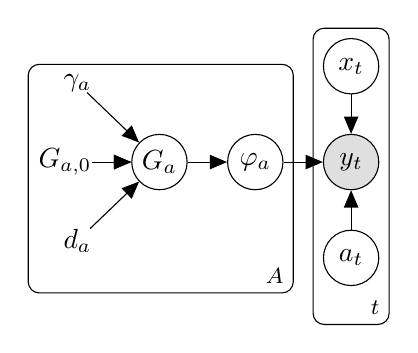
\begin{tikzpicture}
	% Nodes
	% Return y
	\node[obs] (y-t) {$y_{t}$};
	% Action a
	\node[latent, below=0.5 of y-t] (a-t) {$a_t$};
	% Context x
	\node[latent, above=0.5 of y-t]  (x-t) {$x_t$};
	% Nonparametric parameters
	\node[latent, left=0.5 of y-t, xshift=0cm] (varphi-a) {$\varphi_{a}$};
	% Nonparametric distribution
	\node[latent, left=0.5 of varphi-a, xshift=0cm] (G-a) {$G_{a}$};
	
	% Hyperparameters
	\node[const, left=0.5 of G-a, yshift=-1.0cm] (d-a) {$d_{a}$} ;
	\node[const, left=0.5 of G-a, yshift=0.0cm]  (G-a0) {$G_{a,0}$} ;
	\node[const, left=0.5 of G-a, yshift=1.0cm] (gamma-a) {$\gamma_{a}$} ;
	
	% Edges
	% Hyperparameters to distribution
	\edge {gamma-a,G-a0} {G-a} ;
	\edge {d-a,G-a0} {G-a} ;
	% Connect distribution to parameters
	\edge {G-a} {varphi-a} ;
	% Connect parameters, context and arm to observation
	\edge {varphi-a,x-t,a-t} {y-t} ;
	
	% Plates
	% Over time
	\plate {t} {(a-t)(x-t)(y-t)} {$t$} ;
	% Over each arm
	\plate {a}{
		(d-a)(gamma-a)(G-a0) % hyperparameters
		(G-a) % distribution
		(varphi-a) % parameters
	} {$A$} ;
\end{tikzpicture}
		}
		\vspace*{-1ex}
		\caption{The Bayesian nonparametric mixture bandit distribution.}
		\label{fig:pgm_nonparametric_bandit}
	\end{center}
	\vspace*{-4ex}
\end{figure}

By allowing each arm of the bandit to draw from a different nonparametric model, we have full flexibility to estimate each per-arm distribution independently, covering MAB cases with distinct reward model classes per-arm. This setting is a very powerful extension of the MAB problem, which has not attracted interest so far.\footnote{An alternative would be to consider a hierarchical nonparametric model~\cite{j-Teh2006,j-Teh2010}, where all arms are assumed to obey the same family of distributions, but only their mixture proportions vary across arms. We provide details of this alternative model in Section~\ref{asec:nonparametric_hierarchical_mixture_model} of the Appendix.}

In this work, we model context-conditional complex reward densities with nonparametric Gaussian mixture models per-arm,
\begin{equation}
y_{t} \sim p(Y|a,x_t,\varphi) = \sum_{k=1}^{K_a} \frac{n_{a,k}-d_a}{n_a+\gamma_a} \cdot \N{Y|x_{t}^\top w_{a,k}, \sigma_{a,k}^2} + \frac{\gamma_a+K_ad_a}{n_a+\gamma_a} \N{Y|x_{t}^\top w_{a,k_{new}}, \sigma_{a,k_{new}}^2} \;.
\label{eq:nonparametric_Gaussian_mixture}
\end{equation}
Each per-arm distribution is modeled independently, \ie $d_a$, $\gamma_a$, $\varphi_{a,k}=\{w_{a,k}, \sigma_{a,k}^2 \}$, and the number of mixtures $K_a$, are per-arm specific parameterizations. Each per-arm and per-mixture emission distribution is a context-conditional Gaussian density
\begin{equation}
p(Y|a,k,x,\varphi_{a,k})=\N{Y|x^\top w_{a,k}, \sigma_{a,k}^2} \;,
\end{equation}
with an expectation that is linearly dependent on the context at time $t$, $\mu_{t,a,k}=x_t^\top w_{a,k}$. The conjugate prior of each of the mixands is a Normal-inverse Gamma
\begin{equation}
G_{a,0}(\varphi_a) = \NIG{w_a, \sigma_a^2 |u_{a,0}, V_{a,0},\alpha_{a,0}, \beta_{a,0}} \;,
\end{equation}
with hyperparameters $\varPhi_{a,0}=\{u_{a,0}, V_{a,0},\alpha_{a,0}, \beta_{a,0}\}$.

Eqn.~\eqref{eq:nonparametric_Gaussian_mixture} describes per-arm nonparametric Gaussian mixture densities, with a Pitman-Yor nonparametric prior as described in Eqn.~\eqref{eq:pitman_yor_mixture}. With this proposed per-arm nonparametric mixture of Gaussian densities, we make a very flexible reward model assumption that automatically adjusts to the observed data: we are nonparametrically estimating per-arm complex reward densities.
The Bayesian nonparametric literature has already established strong convergence results on the density estimation properties of these models: for a wide class of continuous distributions, the nonparametric posterior converges to the true data-generating density, under mild regularity conditions~\cite{j-Ghosal1999, j-Lijoi2004, j-Tokdar2006, j-Ghosal2007, j-Bhattacharya2010, j-Pati2013}.
 
At every interaction of the MAB with the world, rewards $y_t$ are \iid drawn from a context dependent unknown distribution of the played arm $y_{t}\sim P(Y|a,x,\thetastar)$, which we here approximate via Bayesian nonparametric mixture models. The reward model class we consider here is a very flexible one, which adjusts its complexity as data are observed~\cite{b-Ghosal2017}.
After observing rewards $y_{1:n}$, and conditioned on the auxiliary assignment variables $z_{1:n}$, the posteriors of per-arm and mixture parameters $\varphi_{a,k}$ follow a Normal-inverse Gamma distribution, $G_{a,n_{a,k}}(\varphi_{a,k})=\NIG{w_{a,k}, \sigma_{a,k}^2 |\varPhi_{a,k,n_{a,k}}}$, with updated hyperparameters $\varPhi_{a,k,n_{a,k}}$ that depend on the number $n_{a,k}$ of rewards observed after playing arm $a$ that are assigned to mixture $k$. That is, $\varPhi_{a,k,n_{a,k}}=\{u_{a,k,n_{a,k}}, V_{a,k,n_{a,k}},\alpha_{a,k,n_{a,k}}, \beta_{a,k,n_{a,k}} \}$ with
\begin{equation}
\hspace*{-1ex}\begin{cases}
V_{a,k,n_{a,k}}^{-1} = x_{1:n} R_{a,k} x_{1:n}^\top + V_{a,0}^{-1} \;,\\
u_{a,k,n_{a,k}}= V_{a,k,n_{a,k}} \left( x_{1:n} R_{a,k} y_{1:n} + V_{a,0}^{-1} u_{a,0}\right) \;, \\
\alpha_{a,k,n_{a,k}} = \alpha_{a,0} + \frac{1}{2} \tr{R_{a,k}} \;, \\
\beta_{a,k,n_{a,k}} = \beta_{a,0} + \frac{1}{2}\left(y_{1:n}^\top R_{a,k}y_{1:n} \right) + \frac{1}{2}\left( u_{a,0}^\top V_{a,0}^{-1} u_{a,0} - u_{a,k,n_{a,k}}^\top V_{a,k,n_{a,k}}^{-1} u_{a,k,n_{a,k}} \right) \; ,
\end{cases}
\label{eq:posterior_hyperparameters}
\end{equation}
where $R_{a,k}\in\Real^{n_a\times n_a}$ is a sparse diagonal matrix with elements $\left[R_{a,k}\right]_{n,n^\prime}=\mathds{1}[a_n=a,z_n=k]$, and $n_{a}=\sum_{k=1}^{K_a} n_{a,k}$, the number of rewards observed after playing arm $a$. The number of mixtures per-arm $K_a$ of the bandit is independently drawn from its own Pitman-Yor process. Note that the above expression can be computed sequentially as data are observed for the played arm.

The predictive emission distribution after marginalization of the parameters $\varphi_{a,k}$, needed for solving Eqn.~\eqref{eq:gibbs_mixture_assignment}, follows a conditional Student-t distribution
\begin{equation}
p_{a,k}(Y|a,x,\varPhi_{a,k}) = \T{Y|\nu_{a,k,y}, m_{a,k,y}, r_{a,k,y}}, \; \text{ with }
\begin{cases}
\nu_{a,k,y}=2\alpha_{a,k} \;, \\
m_{a,k,y} = x^\top u_{a,k} \;, \\
r_{a,k,y}^2 = \frac{\beta_{a,k}}{\alpha_{a,k}} (1+x^\top V_{a,k} x) \; .
\end{cases}
\label{eq:predictive_emission_univariate}
\end{equation}
The hyperparameters $\varPhi_{a,k}$ above are those of the prior $\varPhi_{a,0}$, or the posterior $\varPhi_{a,k,n_{a,k}}$, depending on whether the predictive density refers to a new mixture $k_{new}$, or a `\textit{seen}' mixture $k$, for which $n_{a,k}$ observations have been already assigned to, respectively.

Similarly, the likelihood of a set of rewards assigned to a per-arm mixture $k$, $Y_{a,k}=y_{1:n}\cdot \mathds{1}[a_n=a,z_n=k]$, given their associated contexts $X_{a,k}=x_{1:n} \cdot \mathds{1}[a_n=a,z_n=k]$, follows the matrix t-distribution
\begin{equation}
\begin{split}
& p(Y_{a,k}|X_{a,k},X_{\backslash a,k},Y_{\backslash a,k},\varPhi_{a,k}) = \MT{Y_{a,k}|\nu_{Y_{a,k}}, M_{Y_{a,k}}, \Psi_{Y_{a,k}}, \Omega_{Y_{a,k}}} \; , \\
& \text{ with }
\begin{cases}
\nu_{Y_{a,k}}=2 \alpha_{a,k} \;, \\
M_{Y_{a,k}}= X_{a,k}^\top u_{a,k} \;, \\
\Psi_{Y_{a,k}} = I_{n_{a,k}} + X_{a,k}^\top V_{a,k} X_{n_{a,k}} \;, \\
\Omega_{Y_{a,k}} = 2 \beta_{a,k} \; .
\end{cases}
\end{split}
\label{eq:predictive_emission_multivariate}
\end{equation}

\subsection{Nonparametric Gaussian mixture model Thompson sampling}
\label{ssec:nonparametric_thompson_sampling}

We leverage the nonparametric Gaussian mixture model described above, and combine it with a posterior sampling MAB policy, \ie Thompson sampling~\cite{j-Russo2018}. The proposed Thompson sampling for contextual bandits with nonparametric Gaussian mixture reward models is presented in Algorithm~\ref{alg:nonparametric_ts}. At each interaction with the world, Thompson sampling decides which arm to play next based on a random parameter sample, drawn from the posterior distribution updated with all the information available at time $t$.

For nonparametric models as in Eqn~\eqref{eq:nonparametric_Gaussian_mixture}, one draws per-arm and per-mixture Gaussian parameters $\varphi_{a,k}$ from the posterior distributions with updated hyperparameters $\varPhi_{a,k,n_{a,k}}$ in Eqn.~\eqref{eq:posterior_hyperparameters}, conditioned on the mixture assignments $z_{1:n}$ determined by the Gibbs sampler in Eqn.~\eqref{eq:gibbs_mixture_assignment} with marginalized densities in Eqns.~\eqref{eq:predictive_emission_univariate} and~\eqref{eq:predictive_emission_multivariate}. Given the inferred sufficient statistics of the assignments (\ie the counts $n_{a,k}$ of rewards observed for arm $a$ and assigned to mixture $k$), and the drawn posterior parameter samples $w_{a,k}^{(t+1)}$, one computes the expected reward for each arm of the nonparametric bandit, \ie
\vspace*{-1ex}
\begin{equation}
\begin{split}
\mu_{t+1,a}(x_{t+1},\varphi_{a}^{(t+1)})&=\sum_{k=1}^{K_a} \frac{n_{a,k}-d_a}{n_a+\gamma_a} \cdot \left(x_{t+1}^\top w_{a,k}^{(t+1)}\right) + \frac{\gamma_a+K_ad_a}{n_a+\gamma_a} \cdot \left(x_{t+1}^\top w_{a,k}^{(t+1)} \right)\; .
\end{split}
\label{eq:nonparametric_expected_reward}
\end{equation}

\subsubsection{Regret bound}
\label{sssec:nonparametric_thompson_sampling_regret_bound}

In order to bound the regret of the proposed algorithm, we leverage asymptotic posterior converge rates, \ie the rate at which the distance between two densities becomes exponentially small as the number of observation grows.

A Thompson sampling based policy computes the probability of each arm being optimal, which is equivalent to the expectation of the optimal arm indicator function with respect to the joint posterior distribution of the expected rewards, \ie
\begin{equation}
\pi(a|x_{t},\HH_{1:t-1})=\Prob{a=\argmax_{a^\prime \in \A} \mu_{t,a^\prime}|p(\mu_t)} = \eValue{p(\mu_t)}{\myind{a=\argmax_{a^\prime \in \A}\mu_{t,a^\prime}|p(\mu_t)}} 
\end{equation}
The posterior $p(\mu_t)$ above is the joint distribution over the expected rewards of all arms: $\mu_{t}=\{\mu_{t,a}\}, \forall a\in \A$. This posterior is a multivariate distribution over all arms of the bandit, \ie of dimension $|\A|$. Note how the indicator function $\myind{a=\argmax_{a^\prime \in \A}\mu_{t,a^\prime}|p(\mu_t)}$ for each arm $a$ requires the posterior over all arms $a^\prime \in \A$ as input.

\begin{lemma}
	The difference in action probabilities between two Thompson sampling policies is bounded by the total-variation between the posterior distributions of their expected rewards, \ie $p(\mu_{t}|h_{1:t})$ and $q(\mu_{t}|h_{1:t})$, respectively,
	\begin{equation}
	\pi(a|p) - \pi(a|q) = \eValue{p}{\myind{a=\argmax_{a^\prime \in \A} \mu_{t,a^\prime}|p}} - \eValue{q}{\myind{a=\argmax_{a^\prime \in \A} \mu_{t,a^\prime}|q}} \leq \delta_{TV}(p,q)
	\nonumber
	\end{equation}
	\label{lemma:total_variation_bounds_diff_policies}
\end{lemma}

We make use of the above lemma to bound the cumulative regret of the proposed Thompson sampling with Dirichlet process mixtures (\ie $d_a=0, \forall a$) of Gaussian distributions, for bandits with true reward densities that meet certain regularity conditions.

\begin{theorem}
	The regret of a Dirichlet process Gaussian mixture model based Thompson sampling algorithm is bounded by
	\begin{equation}
	R_T	=\eValue{}{\sum_{t=1}^T y_{t,\astar_t}-y_{t,a_t} } \leq 2 C_A A \sqrt{T} (C_p + C_{\ptilde} (\log T)^\kappa ) = O(A \log^\kappa T \sqrt{T}) \; ,
	\nonumber
	\end{equation}
	where the expectations are taken over the unknown rewards, the random actions of the stochastic policies, and the true $\pstar$ reward models that meet mild regularity conditions. 
	\label{th:regret_bound}
\end{theorem}
The proofs of Lemma~\ref{lemma:total_variation_bounds_diff_policies} and Theorem~\ref{th:regret_bound} are provided in Section \ref{asec:nonparametric_thompson_sampling_regret_bound} of the Appendix. The proof of Theorem~\ref{th:regret_bound} results from bounding the regret introduced by two factors: the first, related to the use of Thompson sampling (\ie a policy that does not know the true parameters of the reward distribution, but has knowledge of the true model class); and the second, that accounts for the convergence of the posterior of a nonparametric model to that of the true data generating distribution. The logarithmic term $\log^\kappa T$ in the bound appears due to the convergence rate of the nonparametric density estimation, where the exponent $\kappa\geq 0$ depends on the tail behavior of the base measure and the associated priors of the Dirichlet process --- see Section \ref{asec:nonparametric_thompson_sampling_regret_bound} of the Appendix and posterior convergence analysis in~\cite{j-Ghosal2001,j-Ghosal2007}.

%Nonparametric TS
%\vspace*{-3ex}
\begin{algorithm}
	\caption{Nonparametric Gaussian mixture model based Thompson sampling}
	\label{alg:nonparametric_ts}
	\begin{algorithmic}[1]
		\STATE {\bfseries Input:} Number of arms $A$
		\STATE {\bfseries Input:} Per-arm model hyperparameters $d_a$, $\gamma_a$, $\varPhi_{a,0}$
		\STATE {\bfseries Input:} Gibbs convergence criteria $\epsilon$ and $Gibbs_{max}$ 
		\STATE $\HH_1=\emptyset$
		\FOR{$t=1, \cdots, T$}
		\STATE Receive context $x_{t+1}$
		\FOR{$a=1, \cdots, A$}
		\STATE Draw parameters from the posterior $\varphi_{a,k}^{(t+1)} \sim G_{a,k,n_{a,k}}(\varPhi_{a,k}), \forall k$, as in Eqn.~\eqref{eq:posterior_hyperparameters}
		\STATE Compute $\mu_{t+1,a}(x_{t+1},\varphi_{a}^{(t+1)})$ as in Eqn.~\eqref{eq:nonparametric_expected_reward}
		\ENDFOR
		\STATE Play arm $\; a_{t+1}=\argmax_{a^\prime \in \A} \mu_{t+1,a^\prime}(x_{t+1},\varphi_{a^\prime}^{(t+1)})$
		\STATE Observe reward $y_{t+1}$
		\STATE $\HH_{1:t+1}=\HH_{1:t} \cup \left\{x_{t+1}, a_{t+1}, y_{t+1}\right\}$
		\WHILE{NOT Gibbs convergence criteria}
		\STATE Update mixture assignments $z_{1:n}$ based on Eqn.~\eqref{eq:gibbs_mixture_assignment}
		\STATE Compute sufficient statistics $n_{a,k}$
		\STATE Update parameter posteriors $\varPhi_{a,k,n_{a,k}}$ based on Eqn.~\eqref{eq:posterior_hyperparameters}
		\ENDWHILE
		\ENDFOR
	\end{algorithmic}
\end{algorithm}

\subsubsection{Computational complexity}
\label{sssec:nonparametric_thompson_sampling_computational_complexity}
The Gibbs sampler in lines 14-18 within Algorithm~\ref{alg:nonparametric_ts} is run $Gibbs_{steps}$ until a stopping criteria is met: either the model likelihood of the sampled chain is stable within an $\epsilon$ margin between steps, or a maximum number of iterations $Gibbs_{max}$ is reached. As new rewards $y_{t+1,a_{t+1}}$ are acquired, updates to assignments $z_{t^\prime,a_{t+1}}$ are done sequentially within the Gibbs sampler for $t^\prime=\{1,\cdots,t+1 | a_{t^\prime}=a_{t+1}\}$ --- only the posterior over the last played armed $a_{t+1}$ is recomputed. Since Eqn.~\eqref{eq:posterior_hyperparameters} can be sequentially computed for each per-arm observation, the computational cost of the Gibbs sampler grows with the number of available observation of the played arm. The overall computational cost is $O(T \cdot Gibbs_{steps})$ per-interaction with the world, \ie per newly observed reward $y_{t+1,a_{t+1}}$.

\vspace*{-2ex}
\paragraph{Practical recommendation:} In general, one should run the Gibbs sampler to full convergence, \ie until the $\epsilon$ likelihood margin is met --- recommended when no computational constraints are in place. However, due to the sequential acquisition of observations in the bandit setting, and the need to only update the posterior for the played arm, the Gibbs sampler is warm-started at each interaction with the world, and good convergence can be achieved in few iterations. The Gibbs sampler is run from a good starting point: the per-arm parameter space that describes all but this newly observed reward $y_{t+1,a_{t+1}}$. In practice, and because of the warm-start, one can limit the number of Gibbs sampler iterations per-MAB interaction to upper-bound the algorithm's complexity to $O(T\cdot Gibbs_{max})$, yet achieve satisfactory performance. We emphasize that we do consider a Gibbs sampler that runs until full convergence, but propose to limit the number of Gibbs iterations as an empirical recommendation with good regret performance, yet upper-bounded computational complexity of $O(T \cdot Gibbs_{max})$ per MAB interaction with the environment.

\section{Evaluation}
\label{sec:evaluation}

We evaluate the performance of the proposed nonparametric mixture model based Thompson sampling in diverse synthetic and realistic datasets.

Results for different parameterizations of contextual linear Gaussian MAB settings (provided in Section~\ref{asec:evaluation_linearGaussian} of the Appendix) show that the proposed method attains same cumulative regret than the Thompson sampling in~\cite{j-Agrawal2012}, which correctly assumes the true underlying contextual linear Gaussian model, and can compute posterior updates in closed form. That is, the proposed nonparametric Thompson sampling method is as good as the analytical alternative: the per-arm posterior densities quickly converge to the true unknown distribution, incurring in no additional regret.

We here focus on more challenging MABs, \ie those where the underlying reward distributions do not fit into the exponential family assumption. The following studied scenarios differ in the amount of mixture overlap and the similarity between arms:
\begin{equation}
\texttt{Scenario A:}\\
\resizebox{0.7\textwidth}{!}{$
\begin{cases}
p_{0}(y|x_t,\theta) = 0.5 \cdot \N{y|x_t^\top (1 \; 1), 1} + 0.5 \cdot \N{y|x_t^\top (2 \; 2), 1}\\
p_{1}(y|x_t,\theta) = 0.3 \cdot \N{y|x_t^\top (0 \; 0), 1} + 0.7 \cdot \N{y|x_t^\top (3 \; 3), 1}
\end{cases}
$}
\nonumber
\end{equation}
\vspace*{-2ex}
\begin{equation}
\texttt{Scenario B:}\\
\resizebox{0.85\textwidth}{!}{$
\begin{cases}
p_{0}(y|x_t,\theta) = \N{y|x_t^\top (1 \; 1), 1}\; ,\\
p_{1}(y|x_t,\theta) = 0.5 \cdot \N{y|x_t^\top (1 \; 1), 1} + 0.5 \cdot \N{y|x_t^\top (2 \; 2), 1}\\
p_{2}(y|x_t,\theta) = 0.3 \cdot \N{y|x_t^\top (0 \; 0), 1} + 0.6 \cdot \N{y|x_t^\top (3 \; 3), 1} + 0.1 \cdot \N{y|x_t^\top (4 \; 4), 1} 
\end{cases}
$}
\nonumber
\end{equation}
%\vspace*{-1ex}
\begin{equation}
\texttt{Scenario C:}\\
\resizebox{0.7\textwidth}{!}{$
\begin{cases}
p_{0}(y|x_t,\theta) = 0.75 \cdot \N{y|x_t^\top (0 \; 0), 1} + 0.25 \cdot \N{y|x_t^\top (0 \; 0), 10} \\
p_{1}(y|x_t,\theta) = 0.75 \cdot \N{y|x_t^\top (2 \; 2), 1} + 0.25 \cdot \N{y|x_t^\top (2 \; 2), 10}
\end{cases}
$}
\nonumber
\end{equation}

The reward distributions of these contextual bandits are Gaussian mixtures dependent on a two dimensional uncorrelated uniform context, \ie $x_{i,t}\sim\U{0,1}$, $i\in\{0,1\}$, $t\in \Natural$. These reward distributions are complex --- not within the exponential family of distributions: they are all multi-modal, unbalanced in \texttt{Scenarios A} and \texttt{B}, and with heavy tails in \texttt{Scenario C}. In \texttt{Scenario A}, there is a significant overlap between arm rewards, with quite unbalanced mixtures for arm 1. \texttt{Scenario B} describes a MAB with different per-arm reward distributions: a linear Gaussian distribution for arm 0, a bi-modal Gaussian mixture for arm 1, and an unbalanced Gaussian mixture with three components for arm 2. Finally, \texttt{Scenario C} models heavy-tailed distributions, where the bandit is subject to outlier rewards.

We recall that, even if each scenario is a different MAB setting --- with diverse model classes per-arm in \texttt{Scenario B} --- our proposed Thompson sampling framework is readily applicable to all. On the contrary, alternative methods, such as those based on Gaussian processes~\cite{ip-Srinivas2010,ip-Gruenewaelder2010,ic-Krause2011} require the specification of the correct model class of the MAB they are targeting. These methods, although interesting and flexible, require knowledge of the true underlying model class (\ie what mean and kernel functions to use) and suffer from model misspecification. 

Here, since there is no alternative algorithm to address all MAB scenarios jointly, we compare our proposed Algorithm~\ref{alg:nonparametric_ts} to an Oracle Thompson sampling: one that knows the true number of underlying mixtures of the problem it is targeted to. Note that this is only possible in simulation, where we have access to the reward generation function. Specifically, each Oracle Thompson sampling uses a Dirichlet distribution with the true underlying dimensionality $K$ per-scenario --- instead of a nonparametric prior on the mixtures --- and follows the Gibbs sampler as explained in Section~\ref{sec:proposed_method}.

For each considered scenario, we compare the performance of our proposed method to that of each per-scenario tuned Oracle Thompson sampling. We reiterate that this is only possible in a simulated environment, as knowing the reward complexity of a MAB beforehand is impractical --- an alternative would be to run multiple model assumptions in parallel, with a subsequent model selection.

Fig.~\ref{fig:linear_gaussian_mixtures} shows the cumulative regret --- as in Eqn.~\eqref{eq:cumulative_regret} --- of the proposed nonparametric mixture model Thompson sampling, along with each per-scenario Oracle Thompson sampling. Due to the capacity of Bayesian nonparametrics to autonomously adjust the complexity of the model to the sequentially observed data, the proposed method can, without any per-scenario tuning  ($d_a=0$ and $\gamma_a=0.1$, $\forall a$, in all the experiments), readily target all of them. 

\begin{figure}[!h]
	\centering
	\begin{subfigure}[c]{0.49\textwidth}
		\vspace*{-2ex}
		\includegraphics[width=\textwidth]{./figs/linearGaussianMixture/hard/cumregret_R3629}
		\vspace*{-4ex}
		\caption{\texttt{Scenario A}.}
		\label{fig:linear_gaussian_mixture_hard}
	\end{subfigure}
	\begin{subfigure}[c]{0.49\textwidth}
		\vspace*{-2ex}
		\includegraphics[width=\textwidth]{./figs/linearGaussianMixture/unbalanced/cumregret_R3641}
		\vspace*{-4ex}
		\caption{\texttt{Scenario B}.}
		\label{fig:linear_gaussian_mixture_unbalanced}
	\end{subfigure}

	\begin{subfigure}[c]{0.49\textwidth}
		\includegraphics[width=\textwidth]{./figs/linearGaussianMixture/heavy/cumregret_R3250}
		\vspace*{-4ex}
		\caption{\texttt{Scenario C}.}
		\label{fig:linear_gaussian_mixture_heavy}
	\end{subfigure}
	\begin{subfigure}[c]{0.49\textwidth}
		\includegraphics[width=\textwidth]{./figs/linearGaussianMixture/heavy/cumregret_R3250_mispecified}
		\vspace*{-4ex}
		\caption{\texttt{Scenario C}, with a mispecified model.}
		\label{fig:linear_gaussian_mixture_mispecified}
	\end{subfigure}
	\vspace*{-1ex}
	\caption{Mean regret (standard deviation shown as shaded region) for at least 1000 independent realizations of the presented methods in all scenarios.}
	\label{fig:linear_gaussian_mixtures}
\vspace*{-1ex}
\end{figure}

Our proposed method not only fits the underlying reward function accurately in all cases, but attains reduced regret as well: \%13 and \%19 cumulative regret reduction at $t=500$ for Scenario A and B, respectively. This is achieved in the most challenging (not in the exponential family) MAB settings: \ie unbalanced and heavy tailed bandit distributions, for bandits with different per-arm distributions, and when compared to a per-scenario Oracle Thompson sampling policy (\ie one that knows the true underlying complexity of the model).
We further highlight the built-in flexibility of the nonparametric method by showing in Fig.~\ref{fig:linear_gaussian_mixture_mispecified} how Thompson sampling with a mispecified model (\ie fitting a unimodal distribution to the heavy-tailed \texttt{Scenario B}) suffers in comparison to the proposed nonparametric method (a \%18 cumulative regret reduction is attained).

The proposed nonparametric generative modeling provides further per-arm reward understanding (by plotting or computing other figures of merit from these distributions), as the learned per-arm posteriors converge to the true posteriors. We note that posterior density convergence does not imply that it is consistent in $K$ --- that is, on data from a finite mixture, nonparametrics do not necessarily concentrate at the true number of components~\cite{j-Miller2014}. However, the goal of the Thompson sampling is to approximate the posterior distribution accurately enough to compute its expected value and draw samples from it, in order to maximize the cumulative expected reward, which the results above show is attained.

Regarding convergence of the Gibbs sampler, we argue in Section~\ref{sssec:nonparametric_thompson_sampling_computational_complexity} that due to the \textit{warm-start} at each interaction with the world, good convergence can be achieved in few iterations. That is, Gibbs sampling inference aligns well with the online nature of bandits, as the sampler is updated only with the reward observed for the last played arm. Because of this incremental availability of observations, the sampler achieves quick convergence (in our experiments, a 1\% log-likelihood relative difference between iterations was usually achieved within 5-10 iterations).

We show in Figure~\ref{fig:cumregret_gibbs} that no significant regret performance improvement is achieved by letting the sampler run for a higher number of iterations. \textit{A good enough} posterior convergence at a limited computational budget is possible because the Gibbs sampler is run, at each interaction with the world, from a good starting point: the per-arm parameter space that describes all but this newly observed reward --- $Gibbs_{max}$ updates over all $t_a$ observations for the played arm are still computed.
Therefore, when computational constraints are appropriate (\eg for real time bandits) limiting the number of Gibbs iterations can still achieve satisfactory cumulative regret.

\begin{figure}[!h]
	\centering
	\includegraphics[width=0.5\textwidth]{./figs/linearGaussianMixture/unbalanced/cumregret_gibbs}
	\caption{Cumulative regret on Scenario B, for different maximum number of Gibbs iterations.}
	\label{fig:cumregret_gibbs}
\vspace*{-1ex}
\end{figure}

We finally evaluate the proposed method in a real application as well, \ie the recommendation of personalized news articles, in a similar fashion as done by~\citet{ic-Chapelle2011}. We picked $A=20$ articles shown during two days in the \textit{Today Module of the Yahoo! Front Page}.
The goal is to choose the most interesting article for each user, by counting the total number of clicks. We evaluated both the proposed nonparametric Gaussian mixture model, and the logistic reward model as proposed in~\cite{ic-Chapelle2011,ic-Dumitrascu2018}. All details about the dataset and the implemented MAB models are provided in Section~\ref{asec:evaluation_yahoo} of the Appendix. We observe in Table~\ref{tab:yahoo_logistic_crt} that the proposed method as in Algorithm~\ref{alg:nonparametric_ts} is able to attain satisfactory averaged CTR in both 20-armed MAB scenarios, without any specific modeling or parameter assumptions.

% CTR table
%%%%%%%%%%%%%%%%%%%%%%%%
%% Table for yahoo data with logistic bandits
%%%%%%%%%%%%%%%%%%%%%%%%
\begin{table}[!ht]
	\begin{center}
		\resizebox*{\textwidth}{!}{
			\begin{tabular}{*{3}{|c}|}
				\hline
				% Header
				Model \cellcolor[gray]{0.6} & CTR\cellcolor[gray]{0.6} & Normalized CTR\cellcolor[gray]{0.6} \\ \hline
				% table starts
				\cellcolor[gray]{0.8} Logistic rewards, static arms & 0.0670 +/- 0.0088 & 1.6095 +/- 0.2115  \\ \hline
				\cellcolor[gray]{0.8} Logistic rewards, time-evolving arms & 0.0655 +/- 0.0082 & 1.5745 +/- 0.2064 \\ \hline
			\end{tabular}
		}
		\caption{CTR results for SMC-based policies on the news article recommendation dataset.
			The normalized CTR is with respect to a random recommendation baseline.}
		\label{tab:yahoo_logistic_crt}
	\end{center}
	\vspace*{-2ex}
\end{table}


We conclude by reiterating that the proposed nonparametric Thompson sampling avoids stringent case-by-case model assumptions, and does not require any parameter tuning for each specific MAB, yet attains competitive regret when faced with distinct MAB reward distributions: the same algorithm is run for contextual Gaussian, logistic, and other complex (not in the exponential family) multi-armed bandits.

\section{Conclusion}
\label{sec:conclusion}

We contribute to the field of sequential decision processes by proposing a nonparametric mixture model based Thompson sampling. We merge the advances in the field of Bayesian nonparametrics with a state of the art MAB policy (\ie Thompson sampling), and allow its extension to complex domains with model uncertainty. The proposed Bayesian algorithm provides flexible modeling of convoluted reward functions with convergence guarantees, and attains the exploration-exploitation trade-off in complex MABs with minimal assumptions. Empirical results show good cumulative regret performance of the proposed nonparametric Thompson sampling in challenging domains, remarkably adjusting to the complexity of the underlying bandit --- and bypassing model mispecification --- in an online fashion. With the ability to sequentially learn the nonparametric mixture model that best approximates the true reward distribution, the proposed method can be applied to diverse MAB settings (without stringent model specifications) and attain reduced regret. A future direction is to tighten the presented regret bound, as well as to apply the proposed method to other real MAB applications where complex models are likely to outperform simpler ones.

%%%%%%%%%%%%%%%%%%%%%%%%%%%%%%%%%%%%%%%%%%%%%%%%%%%%%%%%%%%%%%%%%%%%%%%%%%%%%%%
% Acknowledgements 
%\section*{Acknowledgements}
%%%%%%%%%%%%%%%%%%%%%%%%%%%%%%%%%%%%%%%%%%%%%%%%%%%%%%%%%%%%%%%%%%%%%%%%%%%%%%%

%%%%%%%%%%%%%%%%%%%%%%%%%%%%%%%%%%%%%%%%%%%%%%%%%%%%%%%%%%%%%%%%%%%%%%%%%%%%%%%
%%% References
% Generate bibliography from the specified bibliography file
%\bibliography{../literature}
% After compiling, include bbl for ArXiv
\documentclass{article}

%%%%%%%%%%%%%%%%%%%%%%%% STYLE INFO %%%%%%%%%%%%%%%%%%%%%%%%
\usepackage[margin=1.5in]{geometry}

%%%%%%%%%%%%%%%%%%%%%%%% IMPORTS %%%%%%%%%%%%%%%%%%%%%%%%
%%%% PACKAGES TO USE
\usepackage[utf8]{inputenc} % allow utf-8 input
\usepackage[T1]{fontenc}    % use 8-bit T1 fonts
\usepackage{hyperref}       % hyperlinks
\usepackage{url}            % simple URL typesetting
\usepackage{booktabs}       % professional-quality tables
\usepackage{amsfonts}       % blackboard math symbols
\usepackage{nicefrac}       % compact symbols for 1/2, etc.
\usepackage{microtype}      % microtypography
\usepackage{enumerate}
% Math related
\usepackage{amsmath}
\usepackage{amsthm} % For proof environment
\usepackage{mathtools}
% Indicator
%\usepackage{bbm} %uses Type3
\usepackage{dsfont} %works with Type1
% Figures and subfigures
\usepackage{graphicx}
\usepackage{caption}
\usepackage{subcaption}
\usepackage{float} %Stay where told
% Tables
\usepackage{booktabs} % for professional tables
\usepackage{multirow} % to be able to have multiple row expanding cell
\usepackage[table]{xcolor}

% Algorithms
\usepackage{algorithm}
\usepackage{algorithmic}
% To draw graphs
\usepackage{tikz}
\usetikzlibrary{bayesnet} % Library for bayesian networks

% Lemmas, Theorems and proofs
\newtheorem{theorem}{Theorem}
\newtheorem{lemma}{Lemma}
% Bibliography
%\usepackage[round,numbers,sort]{natbib} % Round parentheses for references ()
\usepackage[numbers,sort]{natbib} % Square parentheses for references []
% Select a .bst file for the style
\bibliographystyle{abbrvnat}
% Reference column balancing
\usepackage{flushend}

%%%% DEFINITIONS-MACROS
% Real line
\def \Real{{\mathbb R}} 
\def \Natural{{\mathbb N}} 
%Expected value
\newcommand{\eValue}[2]{\mathbb{E}_{#1}\left\{ #2 \right\}}
\newcommand{\Prob}[1]{\mathbb{P}\left( #1 \right)}
% Kullback-Leibler
\newcommand{\KL}[2]{\mathrm{KL}\left( #1 \| #2\right)}
% My small matrix
\newcommand{\mySmallMatrix}[1]{\left(\begin{smallmatrix} #1 \end{smallmatrix}\right)}
%Determinant
\newcommand{\mydet}[1]{\left| #1 \right|}
% My indicator function
\newcommand{\myind}[1]{\ind{}\left[#1\right]}
% d in integral
\newcommand{\dd}[1]{\mathrm{d} #1}
% TK
\newcommand{\TK}[1]{\textcolor{red}{TK: #1}}

% Useful in Bandits
\newcommand{\A}{\mathcal{A}}
\newcommand{\Astar}{A^*}
\newcommand{\astar}{a^*}
\newcommand{\pstar}{p^*}
\newcommand{\pistar}{\pi^*}
\newcommand{\Atilde}{\tilde{A}}
\newcommand{\atilde}{\tilde{a}}
\newcommand{\ptilde}{\tilde{p}}
\newcommand{\pitilde}{\tilde{\pi}}
\newcommand{\thetastar}{\theta^*}
\newcommand{\thetatilde}{\tilde{\theta}}
\newcommand{\Y}{\mathcal{Y}}
\newcommand{\HH}{\mathcal{H}}

% Abbreviations
\newcommand{\iid}{i.i.d. }
\newcommand{\ie}{i.e., }
\newcommand{\Ie}{I.e., }
\newcommand{\eg}{e.g., }
\newcommand{\Eg}{E.g., }
\newcommand{\etAl}{et al.\xspace}

%Distributions
\newcommand{\N}[1]{\mathcal{N}\left( #1\right)}
\newcommand{\MN}[1]{\mathcal{MN}\left( #1\right)}
\newcommand{\T}[1]{\mathcal{T}\left( #1\right)}
\newcommand{\MT}[1]{\mathcal{MT}\left( #1\right)}
\newcommand{\Dir}[1]{{\rm Dir\left( #1\right)}}
\newcommand{\Mult}[1]{{\rm Mult}\left( #1\right)}
\newcommand{\Cat}[1]{{\rm Cat}\left( #1\right)}
\newcommand{\Bin}[1]{{\rm Bin}\left( #1\right)}
\newcommand{\IG}[1]{{\rm IG}\left( #1\right)}
\newcommand{\NIG}[1]{{\rm NIG}\left( #1\right)}
\newcommand{\NIX}[1]{{\rm NIX}\left( #1\right)}
\newcommand{\IW}[1]{{\rm IW}\left( #1\right)}
\newcommand{\NIW}[1]{{\rm NIW}\left( #1\right)}
\newcommand{\Beta}[1]{{\rm Beta}\left( #1\right)}
\newcommand{\Ber}[1]{{\rm Ber}\left( #1\right)}
\newcommand{\U}[1]{\mathcal{U}\left( #1\right)}

%Others
\newcommand{\eqd}{\stackrel{d}{=}} % equal in distribution/law/measure
\newcommand{\abs}[1]{|{#1}|}
\newcommand{\argmax}{\mathop{\mathrm{argmax}}}
\newcommand{\argmin}{\mathop{\mathrm{argmin}}}
\newcommand{\var}{\textrm{Var}}
\newcommand{\cov}{\textrm{Cov}}
\newcommand{\Var}{\mathbb{V}\mathrm{ar}}
\newcommand{\Cov}{\mathrm{Cov}}
\newcommand{\tr}[1]{\mathrm{tr}\left\{ #1 \right\}} % trace
\newcommand{\diag}{\mathrm{diag}}
\newcommand{\ind}[1]{\mathds{1}_{#1}} % Indicator function
\newcommand{\kl}{\textrm{KL}}
\newcommand{\indep}{{\;\bot\!\!\!\!\!\!\bot\;}}
\newcommand{\eps}{\varepsilon}
%%%%%%%% end iurteaga %%%%%%%%
% Whether to add appendix or not
\def\addappendix{}

\title{Nonparametric Gaussian Mixture Models for the Multi-Armed Contextual Bandit}
\author{ I\~{n}igo Urteaga and Chris H.~Wiggins\\
	{\sf \{inigo.urteaga, chris.wiggins\}@columbia.edu} \\\\
	Department of	Applied Physics and Applied Mathematics\\
	Data Science Institute\\
	Columbia University\\
	New York City, NY 10027
}


\begin{document}

\maketitle

\begin{abstract}
We here adopt Bayesian nonparametric mixture models to extend multi-armed bandits in general, and Thompson sampling in particular, to complex scenarios where there is reward model uncertainty.
The multi-armed bandit is a sequential allocation task where an agent must learn a policy that maximizes long term payoff, where only the reward of the played arm is observed at each interaction with the world. In the stochastic bandit setting, at each interaction, the reward for the selected action is generated from an unknown distribution. Thompson sampling is a generative and interpretable multi-armed bandit algorithm that has been shown both to perform well in practice, and to enjoy optimality properties for certain reward functions. Nevertheless, Thompson sampling requires knowledge of the true reward model, for calculation of expected rewards and sampling from its parameter posterior. In this work, we extend Thompson sampling to complex scenarios where there is model uncertainty, by adopting a very flexible set of reward distributions: nonparametric Gaussian mixture models. The generative process of Bayesian nonparametric mixtures naturally aligns with the Bayesian modeling of multi-armed bandits: the nonparametric model autonomously determines its complexity in an online fashion, as new rewards are observed for the played arms. By characterizing each arm's reward distribution with independent Dirichlet process mixtures and per-mixture parameters, the proposed method sequentially learns the model that best approximates the true underlying reward distribution, achieving successful performance in synthetic and real datasets. Our contribution is valuable for practical scenarios, as it avoids stringent case-by-case model specifications, and yet attains reduced regret in diverse bandit settings.
\end{abstract}

\section{Introduction}
\label{sec:introduction}

%Recent advances in reinforcement learning~\cite{j-Gosavi2009} have sparked renewed interest in sequential decision making.
Sequential decision making aims to optimize interactions with the world (exploit), while simultaneously learning how the world operates (explore). Its origins can be traced back to the beginning of the past century, with important contributions within the field of statistics by~\citet{j-Thompson1935} and later~\citet{j-Robbins1952}.

The multi-armed bandit (MAB) is a natural abstraction for a wide variety of real-world challenges that require learning while simultaneously maximizing rewards~\cite{j-Lai1985, b-Lattimore2019}. The name `bandit' finds its origin in the playing strategy one must devise when facing a row of slot machines. The contextual MAB, where at each interaction with the world side information (known as `context') is available, is a natural extension of the bandit problem. Recently, a renaissance of the study of MAB algorithms has flourished~\cite{j-Agrawal2011,ip-Maillard2011}, and it has attracted interest from industry as well, due to its impact in digital advertising and products~\cite{j-Li2010, ic-Chapelle2011}. 

\citet{j-Thompson1933} sampling, also known as posterior sampling~\cite{j-Russo2014}, provides an elegant approach that tackles the exploration-exploitation dilemma in MABs. It updates a posterior over expected rewards for each arm, and chooses actions based on the probability that they are optimal. It has been empirically and theoretically proven to perform competitively for MAB models within the exponential family~\cite{ic-Chapelle2011,j-Agrawal2012,j-Agrawal2012a,ic-Korda2013}. Besides, its applicability to the more general reinforcement learning setting of Markov Decision Processes~\cite{j-Burnetas1997} has recently tracked momentum as well~\cite{ip-Gopalan2015,ic-Ouyang2017}.
Thompson sampling and the Bayesian approach to the MAB problem facilitate not only generative and interpretable modeling, but sequential and batch processing as well.
A Thompson sampling policy requires access to posterior samples of the model. Unfortunately, maintaining such posterior is intractable for distributions not in the exponential family~\cite{ic-Korda2013,j-Russo2018}.

Developing practical MAB methods to balance exploration and exploitation in complex domains remains largely unsolved.
In an effort to extend Thompson sampling to more complex scenarios, researchers have considered other flexible reward functions and Bayesian inference.
Recent approaches have embraced Bayesian neural networks and approximate inference for Thompson sampling. Variational methods, stochastic mini-batches, and Monte Carlo techniques have been studied for uncertainty estimation of reward posteriors~\cite{ip-Blundell2015, ic-Kingma2015, j-Lipton2016, ic-Osband2016, ip-Li2016}.

~\citet{ip-Riquelme2018} have recently benchmarked such techniques and reported that neural networks with approximate inference, even if successful for supervised learning, under-perform in the MAB setting. In particular,~\citet{ip-Riquelme2018} emphasize the issue of adapting the slow convergence uncertainty estimates of neural net based methods to MABs. In parallel, others have focused on extending Thompson sampling by targeting alternative classes of reward functions, such as approximating the unknown bandit reward functions with Gaussian mixture models~\cite{ip-Urteaga2018}.

Our contribution here is on exploiting Bayesian nonparametric mixture models for Thompson sampling to perform MAB optimization. Bayesian nonparametrics~\cite{j-Gershman2012} have been considered within the MAB setting for continuous action choices via Gaussian processes (GPs)~\cite{ip-Srinivas2010,ip-Gruenewaelder2010,ic-Krause2011}, or to allow for an unknown yet countable number of actions via hierarchical Pitman-Yor processes~\cite{j-Battiston2018}.

GPs are powerful nonparametric methods for modeling distributions over non-linear continuous functions~\cite{b-Rasmussen2005}, and have been used to model a continuum of MAB actions~\cite{ic-Krause2011}. Inference with GPs is computationally demanding --- it scales cubically in the number of observations --- limiting their applicability to the online setting, even if advancements such as pseudo-observations~\cite{ic-Snelson2006} or variational inference~\cite{ip-Titsias2009} can mitigate these shortcomings. 

Alternatively, \citet{j-Battiston2018} consider MABs with a discrete but unknown action space, and propose a hierarchical Pitman-Yor process for the unknown populations, with per-arm Bernoulli reward distributions. In this work, we are not interested in a nonparametric prior over arms (with specific per-arm reward distributions), but in sequential decision making with a discrete set of actions, for which there is uncertainty on the per-arm reward model.

We here propose to combine the flexibility of Bayesian nonparametrics with the large hypothesis space of mixture models, to address complex MABs.

In many contexts, a countably infinite mixture is a very realistic model to assume, and has been shown to succeed in modeling a diversity of phenomena~\cite{j-Gershman2012}. Nonparametric processes are useful priors for Bayesian density estimation. Within such framework, one uses nonparametric prior distributions over the mixing proportions, such as Dirichlet or Pitman-Yor processes~\cite{j-Teh2010}, which not only do not explicitly specify the number of mixtures, but allow for an unbounded number of mixtures to appear as data are observed. The important issue of nonparametric posterior consistency, with converge guarantees for a wide class of mixture models, has already been settled~\cite{j-Ghosal1999, j-Ghosal2001, j-Lijoi2004, j-Ghosal2007}.

In this work, we model each of the MAB arms with flexible per-arm nonparametric mixture models, \ie the complex unknown mapping of the observed rewards is estimated with nonparametric context-conditional Gaussian mixture models. By means of a nonparametric Gaussian mixture model, we can accurately approximate continuous reward distributions, yet have analytically tractable inference and online update rules, which allow for sequential adjustment of the complexity of the model to the observed data. For learning such a nonparametric distribution within the contextual MAB setting, we leverage the well-established advances in Markov chain Monte Carlo methods for Bayesian nonparametric models~\cite{j-Neal2000}. The generative interpretation of Bayesian nonparametric processes aligns well with the sequential nature of the MAB problem. To the best of our knowledge, no other work uses Bayesian nonparametric mixtures to model per-arm reward functions in contextual MABs.

The contributions of this work are:
\begin{enumerate}
	\item To propose a flexible Thompson sampling based method that learns the nonparametric mixture that best approximates the true, but unknown, underlying reward distribution per-arm, adjusting its complexity as it sequentially observes data.
	\item To provide a regret bound of order $O(A \log^\kappa T \sqrt{T})$ for the proposed Thompson sampling algorithm that assumes a Dirichlet process Gaussian mixture model.
	\item To demonstrate empirically that the proposed nonparametric Thompson sampling method is as good as the analytical alternative in MABs with Gaussian contextual rewards: the per-arm nonparametric posterior densities quickly converge to the true unknown distribution, incurring in no additional regret.
	\item To show empirically how the proposed nonparametric method attains reduced regret in complex MABs --- with different and unknown per-arm distributions not in the exponential family --- when compared to an Oracle Thompson sampling policy, \ie one that knows the true underlying model class.
\end{enumerate}

These contributions are valuable for practical MAB scenarios in the presence of model uncertainty, as it avoids stringent case-by-case reward model design choices --- bypassing model mispecification --- and yet attains reduced regret.

\section{Background}
\label{sec:background}

\subsection{Multi-armed bandits}
\label{ssec:background_mab}
A multi-armed bandit is a real time sequential decision process in which, at each interaction with the world, an agent selects an action $a\in \A$ according to a policy targeted to maximize cumulative rewards over time, balancing exploration and exploitation.

The rewards observed by the agent are \iid drawn from the true outcome distribution $\pstar(Y)$, itself randomly drawn from the family of distributions $\mathcal{P}$. We denote by $p_a^*(Y)=p(Y|a)$ the conditional distribution of arm $a$, from which outcomes $y_{t,a}$ are drawn: $y_{t,a}\sim \pstar(Y|a)$.\footnote{Random variables are capitalized, their realizations denoted in lower-case.} These distributions are often parameterized by $\theta \in \Theta$, \ie $\mathcal{P}=\{p(\theta)\}_{\theta \in \Theta}$, where the true reward distribution corresponds to a unique $\theta^* \in \Theta$ : $\pstar(Y)=p(Y|\thetastar)$. Without loss of generality, we will relate to the parametric notation hereafter, and following the Bayesian setting, specify a prior over the parameters $p(\theta|\alpha)$ with hyperparameters $\alpha$ when necessary.

In the contextual MAB, one must decide at each time $t$, which arm $a_{t}$ to play based on the available context, \eg $x_{t}\in\Real^{d}$, where the observed reward for the played arm $y_{t,a_{t}}$ is drawn from the unknown reward distribution conditioned on the context, \ie $y_{t,a_t}\sim p(Y|a_t,x_t,\thetastar)$. Given the true model, the optimal action is $a_t^* = \argmax_{a \in \A} \mu_{t,a}(x_t,\thetastar)$, where $\mu_{t,a}(x_t,\thetastar)=\eValue{Y}{Y|a,x_t,\thetastar}$ is the conditional expectation of each arm, given the context at time $t$, and the true parameters $\theta^*$.

The challenge in the contextual MAB is the lack of knowledge about the reward-generating distribution, \ie uncertainty about $\thetastar$ induces uncertainty about the true optimal action $a_t^*$. One needs to simultaneously learn the properties of the reward distribution, and sequentially decide which action to take next. MAB policies choose the next arm to play, with the goal of maximizing the expected reward, based upon the history observed. Previous history contains the set of given contexts, played arms, and observed rewards up to time $t$, denoted as $\HH_{1:t}=\left\{x_{1:t}, a_{1:t}, y_{1:t}\right\}$, with $x_{1:t} \equiv (x_1, \cdots , x_t)$, $a_{1:t} \equiv (a_1, \cdots , a_t)$ and $y_{1:t} \equiv (y_{1,a_1}, \cdots , y_{t,a_t})$.

We use $\pi(a)$ to denote a bandit policy, which is in general stochastic on its choices of $a\in\A$. The goal of a policy is to maximize its cumulative reward, or equivalently, to minimize the cumulative regret --- the loss incurred due to not knowing the best arm $a_t^*$ at each time $t$ --- \ie $R_T=\sum_{t=1}^T y_{t,\astar_t}-y_{t,a_t}$, where $a_t$ denotes the arm picked by the policy. We study the \emph{expected} cumulative regret at time horizon $T$,
\begin{equation}
R_T=\eValue{}{\sum_{t=1}^T y_{t,\astar_t}-y_{t,a_t} } \; ,
\label{eq:cumulative_regret}
\end{equation}
where the expectation is taken over the randomness in the outcomes $Y$, the arm selection policy $\pi(\cdot)$, and the uncertainty in the true model $\thetastar$.

We focus on Thompson sampling~\cite{j-Russo2018}, a MAB policy that chooses what arm to play next in proportion to its probability of being optimal, \ie $\pi(a) = \Prob{a=a_{t+1}^*|x_{t+1}, \HH_{1:t}, \theta}$, where the uncertainty over the unknown parameters must be accounted for. Specifically, unknown parameters $\theta$  are modeled as random variables with appropriate priors, and the goal is to marginalize over their posterior probability after observing  history $\HH_{1:t}$ up to time instant $t$, \ie
\vspace*{-1ex}
\begin{equation}
\begin{split}
\pi(a|x_{t+1},\HH_{1:t})&=\Prob{a=a_{t+1}^*|x_{t+1},\HH_{1:t}} = \int \Prob{a=a_{t+1}^*|x_{t+1},\HH_{1:t},\theta} p(\theta|\HH_{1:t}) \dd{\theta} \\
&=\int \myind{a=\argmax_{a^\prime \in \A} \mu_{t+1,a^\prime}(x_{t+1},\theta)} p(\theta|\HH_{1:t}) \dd{\theta} \; .
\end{split}
\label{eq:theta_unknown_pr_arm_optimal}
\end{equation}

The above integral can not be solved exactly, even when the parameter posterior update is analytically tractable. Instead, Thompson sampling draws a random parameter sample $\theta^{(t+1)}$ from the updated posterior, and picks the arm that maximizes the expected reward given such drawn parameter sample
\begin{equation}
\pi(a|x_{t+1},\HH_{1:t})=\myind{a=\argmax_{a^\prime \in \A} \mu_{t+1,a^\prime}(x_{t+1},\theta^{(t+1)})}, \text{ with } \; \theta^{(t+1)} \sim p(\theta|\HH_{1:t}) .
\nonumber
\end{equation}

Computing the expectations above, as well as drawing posterior parameters, is attainable for reward models $p(Y|\theta)$ within the exponential family~\cite{ic-Korda2013, j-Russo2018}. In practice however, knowledge of the true reward model is illusory. In the following, we propose Bayesian nonparametric mixture models per-arm, as tractable yet performant distributions for estimating unknown reward functions in MAB settings where there is uncertainty about the reward model.

\subsection{Bayesian nonparametric mixture models}
\label{ssec:background_nonparametric_mixture_model}

Bayesian nonparametric mixture models provide a powerful density estimation framework that adjust model complexity in response to the data observed~\cite{b-Ghosal2017}. The combination of mixture models with Bayesian nonparametrics embodies a large hypothesis space, which can arbitrarily approximate continuous distributions~\cite{j-Ghosal1999, j-Ghosal2001, j-Lijoi2004, j-Ghosal2007}. Bayesian nonparametric mixture models describe countably infinite mixture distributions, which are very flexible assumptions suited for many practical settings~\cite{b-Ghosal2017}. A variety of Bayesian nonparametric alternatives have been studied --- we refer to~\citet{j-Gershman2012} for a detailed literature review of such models, and how they can be used in practice.

We here focus on the Pitman-Yor process, a stochastic process whose sample path is a probability distribution, \ie a generalization of Bayesian nonparametric models from where a drawn random sample is an infinite discrete probability distribution. We succinctly summarize the generative process and the basics for its inference here (see~\cite{j-Teh2010} for further details). A Pitman-Yor mixture model, with discount parameter $0 \leq d < 1$ and concentration parameter $\gamma > -d$, is described by the following generative process.

Mixture parameters are drawn from the Pitman-Yor process, \ie $\varphi_n \sim G=PY(d, \gamma, G_0)$, where $G_0$ is the base measure. We write $G_0(\varphi)=G(\varphi|\varPhi_0)$ and $G_n(\varphi)=G(\varphi|\varPhi_n)$ for the prior and posterior distribution of the parameter set $\varphi$, respectively. $\varPhi_0$ are the prior hyperparameters of the base emission distribution, and $\varPhi_n$ the posterior parameters after $n$ observations. Equivalently, the process can be described as 
\begin{equation}
\varphi_{n+1}|\varphi_{1:n}, d, \gamma, G_0 \sim \sum_{k=1}^{K} \frac{n_k-d}{n+\gamma}\delta_{\varphi_k} + \frac{\gamma+Kd}{n+\gamma}G_0 \; ,
\label{eq:pitman_yor_mixture}
\end{equation}
where $n_k$ refers to the number of observations assigned to mixture $k$, and $n=\sum_{k=1}^Kn_k$. After $n$ observations, there are $K$ already `\textit{seen}' mixtures, and a non-zero probability $\frac{\gamma+Kd}{n+\gamma}$ of observing a new mixture $k_{new}$ drawn from the base measure.
The observation $y_{n+1}$ is drawn from the emission distribution parameterized by its corresponding mixture parameters, \ie $y_{n+1} \sim p(Y|\varphi_{n+1})$.

The Dirichlet process can be readily obtained from Eqn.~\eqref{eq:pitman_yor_mixture} by using $d=0$. The discount parameter gives the Pitman-Yor process more flexibility over tail behavior: the Dirichlet process has exponential tails, whereas the Pitman-Yor can have power-law tails.

For analysis and inference of these models, one incorporates auxiliary latent variables $z_n$. These are categorical variables, where $z_{n}=k$ if observation $y_n$ is drawn from mixture $k$, and their joint posterior factorizes $p(z_{1:n}|\gamma) = \prod_{i=1}^n p(z_i|z_{1:n-1},\gamma)$.

To compute the full joint likelihood of assignments and observations, one must consider the emission distribution of the Pitman-Yor process with parameters $\varPhi$, \ie $p(y_{1:n},z_{1:n}|\gamma, \varPhi) = p(y_{1:n}|z_{1:n}, \varPhi) p(z_{1:n}|\gamma)$.

For inference, given observations $y_{1:n}$, of the unknown latent variables and parameters, one derives a Gibbs sampler that iterates between sampling mixture assignments $z_{1:n}$, and updating the emission distribution parameter posterior $G_n(\varphi)$ --- \citet{j-Teh2010} provide a detailed explanation of the procedure.

The conditional distributions of observation assignments $z_n$ to already drawn mixtures $k\in\{1, \cdots, K\}$, and a new `\textit{unseen}' mixture $k_{new}$ follow
\begin{equation}
\begin{cases}
p(z_{n+1}=k|y_{n+1},y_{1:n},z_{1:n}, \gamma, G_0) \propto \frac{n_k-d}{n+\gamma} \int_{\varphi} p(y_{n+1}|\varphi) G_n(\varphi) \dd{\varphi}\; ,\\
p(z_{n+1}=k_{new}|y_{n+1},y_{1:n},z_{1:n}, \gamma, G_0) \propto \frac{\gamma+K d}{n+\gamma} \int_{\varphi} p(y_{n+1}|\varphi) G_0(\varphi) \dd{\varphi} \; .
\end{cases}
\label{eq:gibbs_mixture_assignment}
\end{equation}

Given these mixture assignments, one updates the parameter posteriors conditioned on $z_{1:n}$ and observations $y_{1:n}$, based on the specific choices of emission distribution and priors, \ie $G_n(\varphi)=G(\varphi|y_{1:n}, z_{1:n},\varPhi_0)$. These also determine the computation of the predictive distribution $p(Y|\varPhi)= \int_{\varphi} p(Y|\varphi) G(\varphi|\varPhi) \dd{\varphi}$ for solving Eqn.~\eqref{eq:gibbs_mixture_assignment}. For analytical convenience, one resorts to emission distributions with their conjugate priors.

\section{Proposed method}
\label{sec:proposed_method}

We propose to combine Bayesian nonparametric mixture models with Thompson sampling for MABs under model uncertainty. We consider an independent set of nonparametric mixture models $G_{a,0}$ per-arm --- with their own hyperparameters $d_a$ and $\gamma_a$ --- allowing for flexible, potentially different, reward distributions for each arm $a\in\A$ of the MAB. The graphical model of the Bayesian nonparametric MAB is rendered in Figure \ref{fig:pgm_nonparametric_bandit}, where we assume complete independence of each arm's reward distribution.

% Nonparametric bandit graphical model
\begin{figure}[!h]
%	\vspace*{-3ex}
	\begin{center}
		\resizebox{0.35\textwidth}{!}{
			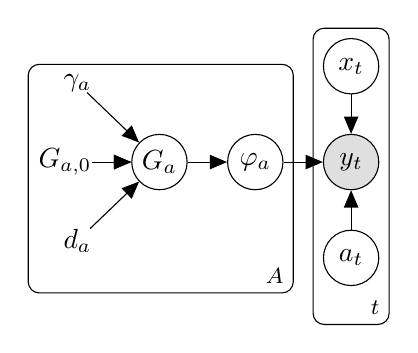
\begin{tikzpicture}
	% Nodes
	% Return y
	\node[obs] (y-t) {$y_{t}$};
	% Action a
	\node[latent, below=0.5 of y-t] (a-t) {$a_t$};
	% Context x
	\node[latent, above=0.5 of y-t]  (x-t) {$x_t$};
	% Nonparametric parameters
	\node[latent, left=0.5 of y-t, xshift=0cm] (varphi-a) {$\varphi_{a}$};
	% Nonparametric distribution
	\node[latent, left=0.5 of varphi-a, xshift=0cm] (G-a) {$G_{a}$};
	
	% Hyperparameters
	\node[const, left=0.5 of G-a, yshift=-1.0cm] (d-a) {$d_{a}$} ;
	\node[const, left=0.5 of G-a, yshift=0.0cm]  (G-a0) {$G_{a,0}$} ;
	\node[const, left=0.5 of G-a, yshift=1.0cm] (gamma-a) {$\gamma_{a}$} ;
	
	% Edges
	% Hyperparameters to distribution
	\edge {gamma-a,G-a0} {G-a} ;
	\edge {d-a,G-a0} {G-a} ;
	% Connect distribution to parameters
	\edge {G-a} {varphi-a} ;
	% Connect parameters, context and arm to observation
	\edge {varphi-a,x-t,a-t} {y-t} ;
	
	% Plates
	% Over time
	\plate {t} {(a-t)(x-t)(y-t)} {$t$} ;
	% Over each arm
	\plate {a}{
		(d-a)(gamma-a)(G-a0) % hyperparameters
		(G-a) % distribution
		(varphi-a) % parameters
	} {$A$} ;
\end{tikzpicture}
		}
		\vspace*{-1ex}
		\caption{The Bayesian nonparametric mixture bandit distribution.}
		\label{fig:pgm_nonparametric_bandit}
	\end{center}
	\vspace*{-4ex}
\end{figure}

By allowing each arm of the bandit to draw from a different nonparametric model, we have full flexibility to estimate each per-arm distribution independently, covering MAB cases with distinct reward model classes per-arm. This setting is a very powerful extension of the MAB problem, which has not attracted interest so far.\footnote{An alternative would be to consider a hierarchical nonparametric model~\cite{j-Teh2006,j-Teh2010}, where all arms are assumed to obey the same family of distributions, but only their mixture proportions vary across arms. We provide details of this alternative model in Section~\ref{asec:nonparametric_hierarchical_mixture_model} of the Appendix.}

In this work, we model context-conditional complex reward densities with nonparametric Gaussian mixture models per-arm,
\begin{equation}
y_{t} \sim p(Y|a,x_t,\varphi) = \sum_{k=1}^{K_a} \frac{n_{a,k}-d_a}{n_a+\gamma_a} \cdot \N{Y|x_{t}^\top w_{a,k}, \sigma_{a,k}^2} + \frac{\gamma_a+K_ad_a}{n_a+\gamma_a} \N{Y|x_{t}^\top w_{a,k_{new}}, \sigma_{a,k_{new}}^2} \;.
\label{eq:nonparametric_Gaussian_mixture}
\end{equation}
Each per-arm distribution is modeled independently, \ie $d_a$, $\gamma_a$, $\varphi_{a,k}=\{w_{a,k}, \sigma_{a,k}^2 \}$, and the number of mixtures $K_a$, are per-arm specific parameterizations. Each per-arm and per-mixture emission distribution is a context-conditional Gaussian density
\begin{equation}
p(Y|a,k,x,\varphi_{a,k})=\N{Y|x^\top w_{a,k}, \sigma_{a,k}^2} \;,
\end{equation}
with an expectation that is linearly dependent on the context at time $t$, $\mu_{t,a,k}=x_t^\top w_{a,k}$. The conjugate prior of each of the mixands is a Normal-inverse Gamma
\begin{equation}
G_{a,0}(\varphi_a) = \NIG{w_a, \sigma_a^2 |u_{a,0}, V_{a,0},\alpha_{a,0}, \beta_{a,0}} \;,
\end{equation}
with hyperparameters $\varPhi_{a,0}=\{u_{a,0}, V_{a,0},\alpha_{a,0}, \beta_{a,0}\}$.

Eqn.~\eqref{eq:nonparametric_Gaussian_mixture} describes per-arm nonparametric Gaussian mixture densities, with a Pitman-Yor nonparametric prior as described in Eqn.~\eqref{eq:pitman_yor_mixture}. With this proposed per-arm nonparametric mixture of Gaussian densities, we make a very flexible reward model assumption that automatically adjusts to the observed data: we are nonparametrically estimating per-arm complex reward densities.
The Bayesian nonparametric literature has already established strong convergence results on the density estimation properties of these models: for a wide class of continuous distributions, the nonparametric posterior converges to the true data-generating density, under mild regularity conditions~\cite{j-Ghosal1999, j-Lijoi2004, j-Tokdar2006, j-Ghosal2007, j-Bhattacharya2010, j-Pati2013}.
 
At every interaction of the MAB with the world, rewards $y_t$ are \iid drawn from a context dependent unknown distribution of the played arm $y_{t}\sim P(Y|a,x,\thetastar)$, which we here approximate via Bayesian nonparametric mixture models. The reward model class we consider here is a very flexible one, which adjusts its complexity as data are observed~\cite{b-Ghosal2017}.
After observing rewards $y_{1:n}$, and conditioned on the auxiliary assignment variables $z_{1:n}$, the posteriors of per-arm and mixture parameters $\varphi_{a,k}$ follow a Normal-inverse Gamma distribution, $G_{a,n_{a,k}}(\varphi_{a,k})=\NIG{w_{a,k}, \sigma_{a,k}^2 |\varPhi_{a,k,n_{a,k}}}$, with updated hyperparameters $\varPhi_{a,k,n_{a,k}}$ that depend on the number $n_{a,k}$ of rewards observed after playing arm $a$ that are assigned to mixture $k$. That is, $\varPhi_{a,k,n_{a,k}}=\{u_{a,k,n_{a,k}}, V_{a,k,n_{a,k}},\alpha_{a,k,n_{a,k}}, \beta_{a,k,n_{a,k}} \}$ with
\begin{equation}
\hspace*{-1ex}\begin{cases}
V_{a,k,n_{a,k}}^{-1} = x_{1:n} R_{a,k} x_{1:n}^\top + V_{a,0}^{-1} \;,\\
u_{a,k,n_{a,k}}= V_{a,k,n_{a,k}} \left( x_{1:n} R_{a,k} y_{1:n} + V_{a,0}^{-1} u_{a,0}\right) \;, \\
\alpha_{a,k,n_{a,k}} = \alpha_{a,0} + \frac{1}{2} \tr{R_{a,k}} \;, \\
\beta_{a,k,n_{a,k}} = \beta_{a,0} + \frac{1}{2}\left(y_{1:n}^\top R_{a,k}y_{1:n} \right) + \frac{1}{2}\left( u_{a,0}^\top V_{a,0}^{-1} u_{a,0} - u_{a,k,n_{a,k}}^\top V_{a,k,n_{a,k}}^{-1} u_{a,k,n_{a,k}} \right) \; ,
\end{cases}
\label{eq:posterior_hyperparameters}
\end{equation}
where $R_{a,k}\in\Real^{n_a\times n_a}$ is a sparse diagonal matrix with elements $\left[R_{a,k}\right]_{n,n^\prime}=\mathds{1}[a_n=a,z_n=k]$, and $n_{a}=\sum_{k=1}^{K_a} n_{a,k}$, the number of rewards observed after playing arm $a$. The number of mixtures per-arm $K_a$ of the bandit is independently drawn from its own Pitman-Yor process. Note that the above expression can be computed sequentially as data are observed for the played arm.

The predictive emission distribution after marginalization of the parameters $\varphi_{a,k}$, needed for solving Eqn.~\eqref{eq:gibbs_mixture_assignment}, follows a conditional Student-t distribution
\begin{equation}
p_{a,k}(Y|a,x,\varPhi_{a,k}) = \T{Y|\nu_{a,k,y}, m_{a,k,y}, r_{a,k,y}}, \; \text{ with }
\begin{cases}
\nu_{a,k,y}=2\alpha_{a,k} \;, \\
m_{a,k,y} = x^\top u_{a,k} \;, \\
r_{a,k,y}^2 = \frac{\beta_{a,k}}{\alpha_{a,k}} (1+x^\top V_{a,k} x) \; .
\end{cases}
\label{eq:predictive_emission_univariate}
\end{equation}
The hyperparameters $\varPhi_{a,k}$ above are those of the prior $\varPhi_{a,0}$, or the posterior $\varPhi_{a,k,n_{a,k}}$, depending on whether the predictive density refers to a new mixture $k_{new}$, or a `\textit{seen}' mixture $k$, for which $n_{a,k}$ observations have been already assigned to, respectively.

Similarly, the likelihood of a set of rewards assigned to a per-arm mixture $k$, $Y_{a,k}=y_{1:n}\cdot \mathds{1}[a_n=a,z_n=k]$, given their associated contexts $X_{a,k}=x_{1:n} \cdot \mathds{1}[a_n=a,z_n=k]$, follows the matrix t-distribution
\begin{equation}
\begin{split}
& p(Y_{a,k}|X_{a,k},X_{\backslash a,k},Y_{\backslash a,k},\varPhi_{a,k}) = \MT{Y_{a,k}|\nu_{Y_{a,k}}, M_{Y_{a,k}}, \Psi_{Y_{a,k}}, \Omega_{Y_{a,k}}} \; , \\
& \text{ with }
\begin{cases}
\nu_{Y_{a,k}}=2 \alpha_{a,k} \;, \\
M_{Y_{a,k}}= X_{a,k}^\top u_{a,k} \;, \\
\Psi_{Y_{a,k}} = I_{n_{a,k}} + X_{a,k}^\top V_{a,k} X_{n_{a,k}} \;, \\
\Omega_{Y_{a,k}} = 2 \beta_{a,k} \; .
\end{cases}
\end{split}
\label{eq:predictive_emission_multivariate}
\end{equation}

\subsection{Nonparametric Gaussian mixture model Thompson sampling}
\label{ssec:nonparametric_thompson_sampling}

We leverage the nonparametric Gaussian mixture model described above, and combine it with a posterior sampling MAB policy, \ie Thompson sampling~\cite{j-Russo2018}. The proposed Thompson sampling for contextual bandits with nonparametric Gaussian mixture reward models is presented in Algorithm~\ref{alg:nonparametric_ts}. At each interaction with the world, Thompson sampling decides which arm to play next based on a random parameter sample, drawn from the posterior distribution updated with all the information available at time $t$.

For nonparametric models as in Eqn~\eqref{eq:nonparametric_Gaussian_mixture}, one draws per-arm and per-mixture Gaussian parameters $\varphi_{a,k}$ from the posterior distributions with updated hyperparameters $\varPhi_{a,k,n_{a,k}}$ in Eqn.~\eqref{eq:posterior_hyperparameters}, conditioned on the mixture assignments $z_{1:n}$ determined by the Gibbs sampler in Eqn.~\eqref{eq:gibbs_mixture_assignment} with marginalized densities in Eqns.~\eqref{eq:predictive_emission_univariate} and~\eqref{eq:predictive_emission_multivariate}. Given the inferred sufficient statistics of the assignments (\ie the counts $n_{a,k}$ of rewards observed for arm $a$ and assigned to mixture $k$), and the drawn posterior parameter samples $w_{a,k}^{(t+1)}$, one computes the expected reward for each arm of the nonparametric bandit, \ie
\vspace*{-1ex}
\begin{equation}
\begin{split}
\mu_{t+1,a}(x_{t+1},\varphi_{a}^{(t+1)})&=\sum_{k=1}^{K_a} \frac{n_{a,k}-d_a}{n_a+\gamma_a} \cdot \left(x_{t+1}^\top w_{a,k}^{(t+1)}\right) + \frac{\gamma_a+K_ad_a}{n_a+\gamma_a} \cdot \left(x_{t+1}^\top w_{a,k}^{(t+1)} \right)\; .
\end{split}
\label{eq:nonparametric_expected_reward}
\end{equation}

\subsubsection{Regret bound}
\label{sssec:nonparametric_thompson_sampling_regret_bound}

In order to bound the regret of the proposed algorithm, we leverage asymptotic posterior converge rates, \ie the rate at which the distance between two densities becomes exponentially small as the number of observation grows.

A Thompson sampling based policy computes the probability of each arm being optimal, which is equivalent to the expectation of the optimal arm indicator function with respect to the joint posterior distribution of the expected rewards, \ie
\begin{equation}
\pi(a|x_{t},\HH_{1:t-1})=\Prob{a=\argmax_{a^\prime \in \A} \mu_{t,a^\prime}|p(\mu_t)} = \eValue{p(\mu_t)}{\myind{a=\argmax_{a^\prime \in \A}\mu_{t,a^\prime}|p(\mu_t)}} 
\end{equation}
The posterior $p(\mu_t)$ above is the joint distribution over the expected rewards of all arms: $\mu_{t}=\{\mu_{t,a}\}, \forall a\in \A$. This posterior is a multivariate distribution over all arms of the bandit, \ie of dimension $|\A|$. Note how the indicator function $\myind{a=\argmax_{a^\prime \in \A}\mu_{t,a^\prime}|p(\mu_t)}$ for each arm $a$ requires the posterior over all arms $a^\prime \in \A$ as input.

\begin{lemma}
	The difference in action probabilities between two Thompson sampling policies is bounded by the total-variation between the posterior distributions of their expected rewards, \ie $p(\mu_{t}|h_{1:t})$ and $q(\mu_{t}|h_{1:t})$, respectively,
	\begin{equation}
	\pi(a|p) - \pi(a|q) = \eValue{p}{\myind{a=\argmax_{a^\prime \in \A} \mu_{t,a^\prime}|p}} - \eValue{q}{\myind{a=\argmax_{a^\prime \in \A} \mu_{t,a^\prime}|q}} \leq \delta_{TV}(p,q)
	\nonumber
	\end{equation}
	\label{lemma:total_variation_bounds_diff_policies}
\end{lemma}

We make use of the above lemma to bound the cumulative regret of the proposed Thompson sampling with Dirichlet process mixtures (\ie $d_a=0, \forall a$) of Gaussian distributions, for bandits with true reward densities that meet certain regularity conditions.

\begin{theorem}
	The regret of a Dirichlet process Gaussian mixture model based Thompson sampling algorithm is bounded by
	\begin{equation}
	R_T	=\eValue{}{\sum_{t=1}^T y_{t,\astar_t}-y_{t,a_t} } \leq 2 C_A A \sqrt{T} (C_p + C_{\ptilde} (\log T)^\kappa ) = O(A \log^\kappa T \sqrt{T}) \; ,
	\nonumber
	\end{equation}
	where the expectations are taken over the unknown rewards, the random actions of the stochastic policies, and the true $\pstar$ reward models that meet mild regularity conditions. 
	\label{th:regret_bound}
\end{theorem}
The proofs of Lemma~\ref{lemma:total_variation_bounds_diff_policies} and Theorem~\ref{th:regret_bound} are provided in Section \ref{asec:nonparametric_thompson_sampling_regret_bound} of the Appendix. The proof of Theorem~\ref{th:regret_bound} results from bounding the regret introduced by two factors: the first, related to the use of Thompson sampling (\ie a policy that does not know the true parameters of the reward distribution, but has knowledge of the true model class); and the second, that accounts for the convergence of the posterior of a nonparametric model to that of the true data generating distribution. The logarithmic term $\log^\kappa T$ in the bound appears due to the convergence rate of the nonparametric density estimation, where the exponent $\kappa\geq 0$ depends on the tail behavior of the base measure and the associated priors of the Dirichlet process --- see Section \ref{asec:nonparametric_thompson_sampling_regret_bound} of the Appendix and posterior convergence analysis in~\cite{j-Ghosal2001,j-Ghosal2007}.

%Nonparametric TS
%\vspace*{-3ex}
\begin{algorithm}
	\caption{Nonparametric Gaussian mixture model based Thompson sampling}
	\label{alg:nonparametric_ts}
	\begin{algorithmic}[1]
		\STATE {\bfseries Input:} Number of arms $A$
		\STATE {\bfseries Input:} Per-arm model hyperparameters $d_a$, $\gamma_a$, $\varPhi_{a,0}$
		\STATE {\bfseries Input:} Gibbs convergence criteria $\epsilon$ and $Gibbs_{max}$ 
		\STATE $\HH_1=\emptyset$
		\FOR{$t=1, \cdots, T$}
		\STATE Receive context $x_{t+1}$
		\FOR{$a=1, \cdots, A$}
		\STATE Draw parameters from the posterior $\varphi_{a,k}^{(t+1)} \sim G_{a,k,n_{a,k}}(\varPhi_{a,k}), \forall k$, as in Eqn.~\eqref{eq:posterior_hyperparameters}
		\STATE Compute $\mu_{t+1,a}(x_{t+1},\varphi_{a}^{(t+1)})$ as in Eqn.~\eqref{eq:nonparametric_expected_reward}
		\ENDFOR
		\STATE Play arm $\; a_{t+1}=\argmax_{a^\prime \in \A} \mu_{t+1,a^\prime}(x_{t+1},\varphi_{a^\prime}^{(t+1)})$
		\STATE Observe reward $y_{t+1}$
		\STATE $\HH_{1:t+1}=\HH_{1:t} \cup \left\{x_{t+1}, a_{t+1}, y_{t+1}\right\}$
		\WHILE{NOT Gibbs convergence criteria}
		\STATE Update mixture assignments $z_{1:n}$ based on Eqn.~\eqref{eq:gibbs_mixture_assignment}
		\STATE Compute sufficient statistics $n_{a,k}$
		\STATE Update parameter posteriors $\varPhi_{a,k,n_{a,k}}$ based on Eqn.~\eqref{eq:posterior_hyperparameters}
		\ENDWHILE
		\ENDFOR
	\end{algorithmic}
\end{algorithm}

\subsubsection{Computational complexity}
\label{sssec:nonparametric_thompson_sampling_computational_complexity}
The Gibbs sampler in lines 14-18 within Algorithm~\ref{alg:nonparametric_ts} is run $Gibbs_{steps}$ until a stopping criteria is met: either the model likelihood of the sampled chain is stable within an $\epsilon$ margin between steps, or a maximum number of iterations $Gibbs_{max}$ is reached. As new rewards $y_{t+1,a_{t+1}}$ are acquired, updates to assignments $z_{t^\prime,a_{t+1}}$ are done sequentially within the Gibbs sampler for $t^\prime=\{1,\cdots,t+1 | a_{t^\prime}=a_{t+1}\}$ --- only the posterior over the last played armed $a_{t+1}$ is recomputed. Since Eqn.~\eqref{eq:posterior_hyperparameters} can be sequentially computed for each per-arm observation, the computational cost of the Gibbs sampler grows with the number of available observation of the played arm. The overall computational cost is $O(T \cdot Gibbs_{steps})$ per-interaction with the world, \ie per newly observed reward $y_{t+1,a_{t+1}}$.

\vspace*{-2ex}
\paragraph{Practical recommendation:} In general, one should run the Gibbs sampler to full convergence, \ie until the $\epsilon$ likelihood margin is met --- recommended when no computational constraints are in place. However, due to the sequential acquisition of observations in the bandit setting, and the need to only update the posterior for the played arm, the Gibbs sampler is warm-started at each interaction with the world, and good convergence can be achieved in few iterations. The Gibbs sampler is run from a good starting point: the per-arm parameter space that describes all but this newly observed reward $y_{t+1,a_{t+1}}$. In practice, and because of the warm-start, one can limit the number of Gibbs sampler iterations per-MAB interaction to upper-bound the algorithm's complexity to $O(T\cdot Gibbs_{max})$, yet achieve satisfactory performance. We emphasize that we do consider a Gibbs sampler that runs until full convergence, but propose to limit the number of Gibbs iterations as an empirical recommendation with good regret performance, yet upper-bounded computational complexity of $O(T \cdot Gibbs_{max})$ per MAB interaction with the environment.

\section{Evaluation}
\label{sec:evaluation}

We evaluate the performance of the proposed nonparametric mixture model based Thompson sampling in diverse synthetic and realistic datasets.

Results for different parameterizations of contextual linear Gaussian MAB settings (provided in Section~\ref{asec:evaluation_linearGaussian} of the Appendix) show that the proposed method attains same cumulative regret than the Thompson sampling in~\cite{j-Agrawal2012}, which correctly assumes the true underlying contextual linear Gaussian model, and can compute posterior updates in closed form. That is, the proposed nonparametric Thompson sampling method is as good as the analytical alternative: the per-arm posterior densities quickly converge to the true unknown distribution, incurring in no additional regret.

We here focus on more challenging MABs, \ie those where the underlying reward distributions do not fit into the exponential family assumption. The following studied scenarios differ in the amount of mixture overlap and the similarity between arms:
\begin{equation}
\texttt{Scenario A:}\\
\resizebox{0.7\textwidth}{!}{$
\begin{cases}
p_{0}(y|x_t,\theta) = 0.5 \cdot \N{y|x_t^\top (1 \; 1), 1} + 0.5 \cdot \N{y|x_t^\top (2 \; 2), 1}\\
p_{1}(y|x_t,\theta) = 0.3 \cdot \N{y|x_t^\top (0 \; 0), 1} + 0.7 \cdot \N{y|x_t^\top (3 \; 3), 1}
\end{cases}
$}
\nonumber
\end{equation}
\vspace*{-2ex}
\begin{equation}
\texttt{Scenario B:}\\
\resizebox{0.85\textwidth}{!}{$
\begin{cases}
p_{0}(y|x_t,\theta) = \N{y|x_t^\top (1 \; 1), 1}\; ,\\
p_{1}(y|x_t,\theta) = 0.5 \cdot \N{y|x_t^\top (1 \; 1), 1} + 0.5 \cdot \N{y|x_t^\top (2 \; 2), 1}\\
p_{2}(y|x_t,\theta) = 0.3 \cdot \N{y|x_t^\top (0 \; 0), 1} + 0.6 \cdot \N{y|x_t^\top (3 \; 3), 1} + 0.1 \cdot \N{y|x_t^\top (4 \; 4), 1} 
\end{cases}
$}
\nonumber
\end{equation}
%\vspace*{-1ex}
\begin{equation}
\texttt{Scenario C:}\\
\resizebox{0.7\textwidth}{!}{$
\begin{cases}
p_{0}(y|x_t,\theta) = 0.75 \cdot \N{y|x_t^\top (0 \; 0), 1} + 0.25 \cdot \N{y|x_t^\top (0 \; 0), 10} \\
p_{1}(y|x_t,\theta) = 0.75 \cdot \N{y|x_t^\top (2 \; 2), 1} + 0.25 \cdot \N{y|x_t^\top (2 \; 2), 10}
\end{cases}
$}
\nonumber
\end{equation}

The reward distributions of these contextual bandits are Gaussian mixtures dependent on a two dimensional uncorrelated uniform context, \ie $x_{i,t}\sim\U{0,1}$, $i\in\{0,1\}$, $t\in \Natural$. These reward distributions are complex --- not within the exponential family of distributions: they are all multi-modal, unbalanced in \texttt{Scenarios A} and \texttt{B}, and with heavy tails in \texttt{Scenario C}. In \texttt{Scenario A}, there is a significant overlap between arm rewards, with quite unbalanced mixtures for arm 1. \texttt{Scenario B} describes a MAB with different per-arm reward distributions: a linear Gaussian distribution for arm 0, a bi-modal Gaussian mixture for arm 1, and an unbalanced Gaussian mixture with three components for arm 2. Finally, \texttt{Scenario C} models heavy-tailed distributions, where the bandit is subject to outlier rewards.

We recall that, even if each scenario is a different MAB setting --- with diverse model classes per-arm in \texttt{Scenario B} --- our proposed Thompson sampling framework is readily applicable to all. On the contrary, alternative methods, such as those based on Gaussian processes~\cite{ip-Srinivas2010,ip-Gruenewaelder2010,ic-Krause2011} require the specification of the correct model class of the MAB they are targeting. These methods, although interesting and flexible, require knowledge of the true underlying model class (\ie what mean and kernel functions to use) and suffer from model misspecification. 

Here, since there is no alternative algorithm to address all MAB scenarios jointly, we compare our proposed Algorithm~\ref{alg:nonparametric_ts} to an Oracle Thompson sampling: one that knows the true number of underlying mixtures of the problem it is targeted to. Note that this is only possible in simulation, where we have access to the reward generation function. Specifically, each Oracle Thompson sampling uses a Dirichlet distribution with the true underlying dimensionality $K$ per-scenario --- instead of a nonparametric prior on the mixtures --- and follows the Gibbs sampler as explained in Section~\ref{sec:proposed_method}.

For each considered scenario, we compare the performance of our proposed method to that of each per-scenario tuned Oracle Thompson sampling. We reiterate that this is only possible in a simulated environment, as knowing the reward complexity of a MAB beforehand is impractical --- an alternative would be to run multiple model assumptions in parallel, with a subsequent model selection.

Fig.~\ref{fig:linear_gaussian_mixtures} shows the cumulative regret --- as in Eqn.~\eqref{eq:cumulative_regret} --- of the proposed nonparametric mixture model Thompson sampling, along with each per-scenario Oracle Thompson sampling. Due to the capacity of Bayesian nonparametrics to autonomously adjust the complexity of the model to the sequentially observed data, the proposed method can, without any per-scenario tuning  ($d_a=0$ and $\gamma_a=0.1$, $\forall a$, in all the experiments), readily target all of them. 

\begin{figure}[!h]
	\centering
	\begin{subfigure}[c]{0.49\textwidth}
		\vspace*{-2ex}
		\includegraphics[width=\textwidth]{./figs/linearGaussianMixture/hard/cumregret_R3629}
		\vspace*{-4ex}
		\caption{\texttt{Scenario A}.}
		\label{fig:linear_gaussian_mixture_hard}
	\end{subfigure}
	\begin{subfigure}[c]{0.49\textwidth}
		\vspace*{-2ex}
		\includegraphics[width=\textwidth]{./figs/linearGaussianMixture/unbalanced/cumregret_R3641}
		\vspace*{-4ex}
		\caption{\texttt{Scenario B}.}
		\label{fig:linear_gaussian_mixture_unbalanced}
	\end{subfigure}

	\begin{subfigure}[c]{0.49\textwidth}
		\includegraphics[width=\textwidth]{./figs/linearGaussianMixture/heavy/cumregret_R3250}
		\vspace*{-4ex}
		\caption{\texttt{Scenario C}.}
		\label{fig:linear_gaussian_mixture_heavy}
	\end{subfigure}
	\begin{subfigure}[c]{0.49\textwidth}
		\includegraphics[width=\textwidth]{./figs/linearGaussianMixture/heavy/cumregret_R3250_mispecified}
		\vspace*{-4ex}
		\caption{\texttt{Scenario C}, with a mispecified model.}
		\label{fig:linear_gaussian_mixture_mispecified}
	\end{subfigure}
	\vspace*{-1ex}
	\caption{Mean regret (standard deviation shown as shaded region) for at least 1000 independent realizations of the presented methods in all scenarios.}
	\label{fig:linear_gaussian_mixtures}
\vspace*{-1ex}
\end{figure}

Our proposed method not only fits the underlying reward function accurately in all cases, but attains reduced regret as well: \%13 and \%19 cumulative regret reduction at $t=500$ for Scenario A and B, respectively. This is achieved in the most challenging (not in the exponential family) MAB settings: \ie unbalanced and heavy tailed bandit distributions, for bandits with different per-arm distributions, and when compared to a per-scenario Oracle Thompson sampling policy (\ie one that knows the true underlying complexity of the model).
We further highlight the built-in flexibility of the nonparametric method by showing in Fig.~\ref{fig:linear_gaussian_mixture_mispecified} how Thompson sampling with a mispecified model (\ie fitting a unimodal distribution to the heavy-tailed \texttt{Scenario B}) suffers in comparison to the proposed nonparametric method (a \%18 cumulative regret reduction is attained).

The proposed nonparametric generative modeling provides further per-arm reward understanding (by plotting or computing other figures of merit from these distributions), as the learned per-arm posteriors converge to the true posteriors. We note that posterior density convergence does not imply that it is consistent in $K$ --- that is, on data from a finite mixture, nonparametrics do not necessarily concentrate at the true number of components~\cite{j-Miller2014}. However, the goal of the Thompson sampling is to approximate the posterior distribution accurately enough to compute its expected value and draw samples from it, in order to maximize the cumulative expected reward, which the results above show is attained.

Regarding convergence of the Gibbs sampler, we argue in Section~\ref{sssec:nonparametric_thompson_sampling_computational_complexity} that due to the \textit{warm-start} at each interaction with the world, good convergence can be achieved in few iterations. That is, Gibbs sampling inference aligns well with the online nature of bandits, as the sampler is updated only with the reward observed for the last played arm. Because of this incremental availability of observations, the sampler achieves quick convergence (in our experiments, a 1\% log-likelihood relative difference between iterations was usually achieved within 5-10 iterations).

We show in Figure~\ref{fig:cumregret_gibbs} that no significant regret performance improvement is achieved by letting the sampler run for a higher number of iterations. \textit{A good enough} posterior convergence at a limited computational budget is possible because the Gibbs sampler is run, at each interaction with the world, from a good starting point: the per-arm parameter space that describes all but this newly observed reward --- $Gibbs_{max}$ updates over all $t_a$ observations for the played arm are still computed.
Therefore, when computational constraints are appropriate (\eg for real time bandits) limiting the number of Gibbs iterations can still achieve satisfactory cumulative regret.

\begin{figure}[!h]
	\centering
	\includegraphics[width=0.5\textwidth]{./figs/linearGaussianMixture/unbalanced/cumregret_gibbs}
	\caption{Cumulative regret on Scenario B, for different maximum number of Gibbs iterations.}
	\label{fig:cumregret_gibbs}
\vspace*{-1ex}
\end{figure}

We finally evaluate the proposed method in a real application as well, \ie the recommendation of personalized news articles, in a similar fashion as done by~\citet{ic-Chapelle2011}. We picked $A=20$ articles shown during two days in the \textit{Today Module of the Yahoo! Front Page}.
The goal is to choose the most interesting article for each user, by counting the total number of clicks. We evaluated both the proposed nonparametric Gaussian mixture model, and the logistic reward model as proposed in~\cite{ic-Chapelle2011,ic-Dumitrascu2018}. All details about the dataset and the implemented MAB models are provided in Section~\ref{asec:evaluation_yahoo} of the Appendix. We observe in Table~\ref{tab:yahoo_logistic_crt} that the proposed method as in Algorithm~\ref{alg:nonparametric_ts} is able to attain satisfactory averaged CTR in both 20-armed MAB scenarios, without any specific modeling or parameter assumptions.

% CTR table
%%%%%%%%%%%%%%%%%%%%%%%%
%% Table for yahoo data with logistic bandits
%%%%%%%%%%%%%%%%%%%%%%%%
\begin{table}[!ht]
	\begin{center}
		\resizebox*{\textwidth}{!}{
			\begin{tabular}{*{3}{|c}|}
				\hline
				% Header
				Model \cellcolor[gray]{0.6} & CTR\cellcolor[gray]{0.6} & Normalized CTR\cellcolor[gray]{0.6} \\ \hline
				% table starts
				\cellcolor[gray]{0.8} Logistic rewards, static arms & 0.0670 +/- 0.0088 & 1.6095 +/- 0.2115  \\ \hline
				\cellcolor[gray]{0.8} Logistic rewards, time-evolving arms & 0.0655 +/- 0.0082 & 1.5745 +/- 0.2064 \\ \hline
			\end{tabular}
		}
		\caption{CTR results for SMC-based policies on the news article recommendation dataset.
			The normalized CTR is with respect to a random recommendation baseline.}
		\label{tab:yahoo_logistic_crt}
	\end{center}
	\vspace*{-2ex}
\end{table}


We conclude by reiterating that the proposed nonparametric Thompson sampling avoids stringent case-by-case model assumptions, and does not require any parameter tuning for each specific MAB, yet attains competitive regret when faced with distinct MAB reward distributions: the same algorithm is run for contextual Gaussian, logistic, and other complex (not in the exponential family) multi-armed bandits.

\section{Conclusion}
\label{sec:conclusion}

We contribute to the field of sequential decision processes by proposing a nonparametric mixture model based Thompson sampling. We merge the advances in the field of Bayesian nonparametrics with a state of the art MAB policy (\ie Thompson sampling), and allow its extension to complex domains with model uncertainty. The proposed Bayesian algorithm provides flexible modeling of convoluted reward functions with convergence guarantees, and attains the exploration-exploitation trade-off in complex MABs with minimal assumptions. Empirical results show good cumulative regret performance of the proposed nonparametric Thompson sampling in challenging domains, remarkably adjusting to the complexity of the underlying bandit --- and bypassing model mispecification --- in an online fashion. With the ability to sequentially learn the nonparametric mixture model that best approximates the true reward distribution, the proposed method can be applied to diverse MAB settings (without stringent model specifications) and attain reduced regret. A future direction is to tighten the presented regret bound, as well as to apply the proposed method to other real MAB applications where complex models are likely to outperform simpler ones.

%%%%%%%%%%%%%%%%%%%%%%%%%%%%%%%%%%%%%%%%%%%%%%%%%%%%%%%%%%%%%%%%%%%%%%%%%%%%%%%
% Acknowledgements 
%\section*{Acknowledgements}
%%%%%%%%%%%%%%%%%%%%%%%%%%%%%%%%%%%%%%%%%%%%%%%%%%%%%%%%%%%%%%%%%%%%%%%%%%%%%%%

%%%%%%%%%%%%%%%%%%%%%%%%%%%%%%%%%%%%%%%%%%%%%%%%%%%%%%%%%%%%%%%%%%%%%%%%%%%%%%%
%%% References
% Generate bibliography from the specified bibliography file
%\bibliography{../literature}
% After compiling, include bbl for ArXiv
\documentclass{article}

%%%%%%%%%%%%%%%%%%%%%%%% STYLE INFO %%%%%%%%%%%%%%%%%%%%%%%%
\usepackage[margin=1.5in]{geometry}

%%%%%%%%%%%%%%%%%%%%%%%% IMPORTS %%%%%%%%%%%%%%%%%%%%%%%%
%%%% PACKAGES TO USE
\usepackage[utf8]{inputenc} % allow utf-8 input
\usepackage[T1]{fontenc}    % use 8-bit T1 fonts
\usepackage{hyperref}       % hyperlinks
\usepackage{url}            % simple URL typesetting
\usepackage{booktabs}       % professional-quality tables
\usepackage{amsfonts}       % blackboard math symbols
\usepackage{nicefrac}       % compact symbols for 1/2, etc.
\usepackage{microtype}      % microtypography
\usepackage{enumerate}
% Math related
\usepackage{amsmath}
\usepackage{amsthm} % For proof environment
\usepackage{mathtools}
% Indicator
%\usepackage{bbm} %uses Type3
\usepackage{dsfont} %works with Type1
% Figures and subfigures
\usepackage{graphicx}
\usepackage{caption}
\usepackage{subcaption}
\usepackage{float} %Stay where told
% Tables
\usepackage{booktabs} % for professional tables
\usepackage{multirow} % to be able to have multiple row expanding cell
\usepackage[table]{xcolor}

% Algorithms
\usepackage{algorithm}
\usepackage{algorithmic}
% To draw graphs
\usepackage{tikz}
\usetikzlibrary{bayesnet} % Library for bayesian networks

% Lemmas, Theorems and proofs
\newtheorem{theorem}{Theorem}
\newtheorem{lemma}{Lemma}
% Bibliography
%\usepackage[round,numbers,sort]{natbib} % Round parentheses for references ()
\usepackage[numbers,sort]{natbib} % Square parentheses for references []
% Select a .bst file for the style
\bibliographystyle{abbrvnat}
% Reference column balancing
\usepackage{flushend}

%%%% DEFINITIONS-MACROS
% Real line
\def \Real{{\mathbb R}} 
\def \Natural{{\mathbb N}} 
%Expected value
\newcommand{\eValue}[2]{\mathbb{E}_{#1}\left\{ #2 \right\}}
\newcommand{\Prob}[1]{\mathbb{P}\left( #1 \right)}
% Kullback-Leibler
\newcommand{\KL}[2]{\mathrm{KL}\left( #1 \| #2\right)}
% My small matrix
\newcommand{\mySmallMatrix}[1]{\left(\begin{smallmatrix} #1 \end{smallmatrix}\right)}
%Determinant
\newcommand{\mydet}[1]{\left| #1 \right|}
% My indicator function
\newcommand{\myind}[1]{\ind{}\left[#1\right]}
% d in integral
\newcommand{\dd}[1]{\mathrm{d} #1}
% TK
\newcommand{\TK}[1]{\textcolor{red}{TK: #1}}

% Useful in Bandits
\newcommand{\A}{\mathcal{A}}
\newcommand{\Astar}{A^*}
\newcommand{\astar}{a^*}
\newcommand{\pstar}{p^*}
\newcommand{\pistar}{\pi^*}
\newcommand{\Atilde}{\tilde{A}}
\newcommand{\atilde}{\tilde{a}}
\newcommand{\ptilde}{\tilde{p}}
\newcommand{\pitilde}{\tilde{\pi}}
\newcommand{\thetastar}{\theta^*}
\newcommand{\thetatilde}{\tilde{\theta}}
\newcommand{\Y}{\mathcal{Y}}
\newcommand{\HH}{\mathcal{H}}

% Abbreviations
\newcommand{\iid}{i.i.d. }
\newcommand{\ie}{i.e., }
\newcommand{\Ie}{I.e., }
\newcommand{\eg}{e.g., }
\newcommand{\Eg}{E.g., }
\newcommand{\etAl}{et al.\xspace}

%Distributions
\newcommand{\N}[1]{\mathcal{N}\left( #1\right)}
\newcommand{\MN}[1]{\mathcal{MN}\left( #1\right)}
\newcommand{\T}[1]{\mathcal{T}\left( #1\right)}
\newcommand{\MT}[1]{\mathcal{MT}\left( #1\right)}
\newcommand{\Dir}[1]{{\rm Dir\left( #1\right)}}
\newcommand{\Mult}[1]{{\rm Mult}\left( #1\right)}
\newcommand{\Cat}[1]{{\rm Cat}\left( #1\right)}
\newcommand{\Bin}[1]{{\rm Bin}\left( #1\right)}
\newcommand{\IG}[1]{{\rm IG}\left( #1\right)}
\newcommand{\NIG}[1]{{\rm NIG}\left( #1\right)}
\newcommand{\NIX}[1]{{\rm NIX}\left( #1\right)}
\newcommand{\IW}[1]{{\rm IW}\left( #1\right)}
\newcommand{\NIW}[1]{{\rm NIW}\left( #1\right)}
\newcommand{\Beta}[1]{{\rm Beta}\left( #1\right)}
\newcommand{\Ber}[1]{{\rm Ber}\left( #1\right)}
\newcommand{\U}[1]{\mathcal{U}\left( #1\right)}

%Others
\newcommand{\eqd}{\stackrel{d}{=}} % equal in distribution/law/measure
\newcommand{\abs}[1]{|{#1}|}
\newcommand{\argmax}{\mathop{\mathrm{argmax}}}
\newcommand{\argmin}{\mathop{\mathrm{argmin}}}
\newcommand{\var}{\textrm{Var}}
\newcommand{\cov}{\textrm{Cov}}
\newcommand{\Var}{\mathbb{V}\mathrm{ar}}
\newcommand{\Cov}{\mathrm{Cov}}
\newcommand{\tr}[1]{\mathrm{tr}\left\{ #1 \right\}} % trace
\newcommand{\diag}{\mathrm{diag}}
\newcommand{\ind}[1]{\mathds{1}_{#1}} % Indicator function
\newcommand{\kl}{\textrm{KL}}
\newcommand{\indep}{{\;\bot\!\!\!\!\!\!\bot\;}}
\newcommand{\eps}{\varepsilon}
%%%%%%%% end iurteaga %%%%%%%%
% Whether to add appendix or not
\def\addappendix{}

\title{Nonparametric Gaussian Mixture Models for the Multi-Armed Contextual Bandit}
\author{ I\~{n}igo Urteaga and Chris H.~Wiggins\\
	{\sf \{inigo.urteaga, chris.wiggins\}@columbia.edu} \\\\
	Department of	Applied Physics and Applied Mathematics\\
	Data Science Institute\\
	Columbia University\\
	New York City, NY 10027
}


\begin{document}

\maketitle

\begin{abstract}
We here adopt Bayesian nonparametric mixture models to extend multi-armed bandits in general, and Thompson sampling in particular, to complex scenarios where there is reward model uncertainty.
The multi-armed bandit is a sequential allocation task where an agent must learn a policy that maximizes long term payoff, where only the reward of the played arm is observed at each interaction with the world. In the stochastic bandit setting, at each interaction, the reward for the selected action is generated from an unknown distribution. Thompson sampling is a generative and interpretable multi-armed bandit algorithm that has been shown both to perform well in practice, and to enjoy optimality properties for certain reward functions. Nevertheless, Thompson sampling requires knowledge of the true reward model, for calculation of expected rewards and sampling from its parameter posterior. In this work, we extend Thompson sampling to complex scenarios where there is model uncertainty, by adopting a very flexible set of reward distributions: nonparametric Gaussian mixture models. The generative process of Bayesian nonparametric mixtures naturally aligns with the Bayesian modeling of multi-armed bandits: the nonparametric model autonomously determines its complexity in an online fashion, as new rewards are observed for the played arms. By characterizing each arm's reward distribution with independent Dirichlet process mixtures and per-mixture parameters, the proposed method sequentially learns the model that best approximates the true underlying reward distribution, achieving successful performance in synthetic and real datasets. Our contribution is valuable for practical scenarios, as it avoids stringent case-by-case model specifications, and yet attains reduced regret in diverse bandit settings.
\end{abstract}

\section{Introduction}
\label{sec:introduction}

%Recent advances in reinforcement learning~\cite{j-Gosavi2009} have sparked renewed interest in sequential decision making.
Sequential decision making aims to optimize interactions with the world (exploit), while simultaneously learning how the world operates (explore). Its origins can be traced back to the beginning of the past century, with important contributions within the field of statistics by~\citet{j-Thompson1935} and later~\citet{j-Robbins1952}.

The multi-armed bandit (MAB) is a natural abstraction for a wide variety of real-world challenges that require learning while simultaneously maximizing rewards~\cite{j-Lai1985, b-Lattimore2019}. The name `bandit' finds its origin in the playing strategy one must devise when facing a row of slot machines. The contextual MAB, where at each interaction with the world side information (known as `context') is available, is a natural extension of the bandit problem. Recently, a renaissance of the study of MAB algorithms has flourished~\cite{j-Agrawal2011,ip-Maillard2011}, and it has attracted interest from industry as well, due to its impact in digital advertising and products~\cite{j-Li2010, ic-Chapelle2011}. 

\citet{j-Thompson1933} sampling, also known as posterior sampling~\cite{j-Russo2014}, provides an elegant approach that tackles the exploration-exploitation dilemma in MABs. It updates a posterior over expected rewards for each arm, and chooses actions based on the probability that they are optimal. It has been empirically and theoretically proven to perform competitively for MAB models within the exponential family~\cite{ic-Chapelle2011,j-Agrawal2012,j-Agrawal2012a,ic-Korda2013}. Besides, its applicability to the more general reinforcement learning setting of Markov Decision Processes~\cite{j-Burnetas1997} has recently tracked momentum as well~\cite{ip-Gopalan2015,ic-Ouyang2017}.
Thompson sampling and the Bayesian approach to the MAB problem facilitate not only generative and interpretable modeling, but sequential and batch processing as well.
A Thompson sampling policy requires access to posterior samples of the model. Unfortunately, maintaining such posterior is intractable for distributions not in the exponential family~\cite{ic-Korda2013,j-Russo2018}.

Developing practical MAB methods to balance exploration and exploitation in complex domains remains largely unsolved.
In an effort to extend Thompson sampling to more complex scenarios, researchers have considered other flexible reward functions and Bayesian inference.
Recent approaches have embraced Bayesian neural networks and approximate inference for Thompson sampling. Variational methods, stochastic mini-batches, and Monte Carlo techniques have been studied for uncertainty estimation of reward posteriors~\cite{ip-Blundell2015, ic-Kingma2015, j-Lipton2016, ic-Osband2016, ip-Li2016}.

~\citet{ip-Riquelme2018} have recently benchmarked such techniques and reported that neural networks with approximate inference, even if successful for supervised learning, under-perform in the MAB setting. In particular,~\citet{ip-Riquelme2018} emphasize the issue of adapting the slow convergence uncertainty estimates of neural net based methods to MABs. In parallel, others have focused on extending Thompson sampling by targeting alternative classes of reward functions, such as approximating the unknown bandit reward functions with Gaussian mixture models~\cite{ip-Urteaga2018}.

Our contribution here is on exploiting Bayesian nonparametric mixture models for Thompson sampling to perform MAB optimization. Bayesian nonparametrics~\cite{j-Gershman2012} have been considered within the MAB setting for continuous action choices via Gaussian processes (GPs)~\cite{ip-Srinivas2010,ip-Gruenewaelder2010,ic-Krause2011}, or to allow for an unknown yet countable number of actions via hierarchical Pitman-Yor processes~\cite{j-Battiston2018}.

GPs are powerful nonparametric methods for modeling distributions over non-linear continuous functions~\cite{b-Rasmussen2005}, and have been used to model a continuum of MAB actions~\cite{ic-Krause2011}. Inference with GPs is computationally demanding --- it scales cubically in the number of observations --- limiting their applicability to the online setting, even if advancements such as pseudo-observations~\cite{ic-Snelson2006} or variational inference~\cite{ip-Titsias2009} can mitigate these shortcomings. 

Alternatively, \citet{j-Battiston2018} consider MABs with a discrete but unknown action space, and propose a hierarchical Pitman-Yor process for the unknown populations, with per-arm Bernoulli reward distributions. In this work, we are not interested in a nonparametric prior over arms (with specific per-arm reward distributions), but in sequential decision making with a discrete set of actions, for which there is uncertainty on the per-arm reward model.

We here propose to combine the flexibility of Bayesian nonparametrics with the large hypothesis space of mixture models, to address complex MABs.

In many contexts, a countably infinite mixture is a very realistic model to assume, and has been shown to succeed in modeling a diversity of phenomena~\cite{j-Gershman2012}. Nonparametric processes are useful priors for Bayesian density estimation. Within such framework, one uses nonparametric prior distributions over the mixing proportions, such as Dirichlet or Pitman-Yor processes~\cite{j-Teh2010}, which not only do not explicitly specify the number of mixtures, but allow for an unbounded number of mixtures to appear as data are observed. The important issue of nonparametric posterior consistency, with converge guarantees for a wide class of mixture models, has already been settled~\cite{j-Ghosal1999, j-Ghosal2001, j-Lijoi2004, j-Ghosal2007}.

In this work, we model each of the MAB arms with flexible per-arm nonparametric mixture models, \ie the complex unknown mapping of the observed rewards is estimated with nonparametric context-conditional Gaussian mixture models. By means of a nonparametric Gaussian mixture model, we can accurately approximate continuous reward distributions, yet have analytically tractable inference and online update rules, which allow for sequential adjustment of the complexity of the model to the observed data. For learning such a nonparametric distribution within the contextual MAB setting, we leverage the well-established advances in Markov chain Monte Carlo methods for Bayesian nonparametric models~\cite{j-Neal2000}. The generative interpretation of Bayesian nonparametric processes aligns well with the sequential nature of the MAB problem. To the best of our knowledge, no other work uses Bayesian nonparametric mixtures to model per-arm reward functions in contextual MABs.

The contributions of this work are:
\begin{enumerate}
	\item To propose a flexible Thompson sampling based method that learns the nonparametric mixture that best approximates the true, but unknown, underlying reward distribution per-arm, adjusting its complexity as it sequentially observes data.
	\item To provide a regret bound of order $O(A \log^\kappa T \sqrt{T})$ for the proposed Thompson sampling algorithm that assumes a Dirichlet process Gaussian mixture model.
	\item To demonstrate empirically that the proposed nonparametric Thompson sampling method is as good as the analytical alternative in MABs with Gaussian contextual rewards: the per-arm nonparametric posterior densities quickly converge to the true unknown distribution, incurring in no additional regret.
	\item To show empirically how the proposed nonparametric method attains reduced regret in complex MABs --- with different and unknown per-arm distributions not in the exponential family --- when compared to an Oracle Thompson sampling policy, \ie one that knows the true underlying model class.
\end{enumerate}

These contributions are valuable for practical MAB scenarios in the presence of model uncertainty, as it avoids stringent case-by-case reward model design choices --- bypassing model mispecification --- and yet attains reduced regret.

\section{Background}
\label{sec:background}

\subsection{Multi-armed bandits}
\label{ssec:background_mab}
A multi-armed bandit is a real time sequential decision process in which, at each interaction with the world, an agent selects an action $a\in \A$ according to a policy targeted to maximize cumulative rewards over time, balancing exploration and exploitation.

The rewards observed by the agent are \iid drawn from the true outcome distribution $\pstar(Y)$, itself randomly drawn from the family of distributions $\mathcal{P}$. We denote by $p_a^*(Y)=p(Y|a)$ the conditional distribution of arm $a$, from which outcomes $y_{t,a}$ are drawn: $y_{t,a}\sim \pstar(Y|a)$.\footnote{Random variables are capitalized, their realizations denoted in lower-case.} These distributions are often parameterized by $\theta \in \Theta$, \ie $\mathcal{P}=\{p(\theta)\}_{\theta \in \Theta}$, where the true reward distribution corresponds to a unique $\theta^* \in \Theta$ : $\pstar(Y)=p(Y|\thetastar)$. Without loss of generality, we will relate to the parametric notation hereafter, and following the Bayesian setting, specify a prior over the parameters $p(\theta|\alpha)$ with hyperparameters $\alpha$ when necessary.

In the contextual MAB, one must decide at each time $t$, which arm $a_{t}$ to play based on the available context, \eg $x_{t}\in\Real^{d}$, where the observed reward for the played arm $y_{t,a_{t}}$ is drawn from the unknown reward distribution conditioned on the context, \ie $y_{t,a_t}\sim p(Y|a_t,x_t,\thetastar)$. Given the true model, the optimal action is $a_t^* = \argmax_{a \in \A} \mu_{t,a}(x_t,\thetastar)$, where $\mu_{t,a}(x_t,\thetastar)=\eValue{Y}{Y|a,x_t,\thetastar}$ is the conditional expectation of each arm, given the context at time $t$, and the true parameters $\theta^*$.

The challenge in the contextual MAB is the lack of knowledge about the reward-generating distribution, \ie uncertainty about $\thetastar$ induces uncertainty about the true optimal action $a_t^*$. One needs to simultaneously learn the properties of the reward distribution, and sequentially decide which action to take next. MAB policies choose the next arm to play, with the goal of maximizing the expected reward, based upon the history observed. Previous history contains the set of given contexts, played arms, and observed rewards up to time $t$, denoted as $\HH_{1:t}=\left\{x_{1:t}, a_{1:t}, y_{1:t}\right\}$, with $x_{1:t} \equiv (x_1, \cdots , x_t)$, $a_{1:t} \equiv (a_1, \cdots , a_t)$ and $y_{1:t} \equiv (y_{1,a_1}, \cdots , y_{t,a_t})$.

We use $\pi(a)$ to denote a bandit policy, which is in general stochastic on its choices of $a\in\A$. The goal of a policy is to maximize its cumulative reward, or equivalently, to minimize the cumulative regret --- the loss incurred due to not knowing the best arm $a_t^*$ at each time $t$ --- \ie $R_T=\sum_{t=1}^T y_{t,\astar_t}-y_{t,a_t}$, where $a_t$ denotes the arm picked by the policy. We study the \emph{expected} cumulative regret at time horizon $T$,
\begin{equation}
R_T=\eValue{}{\sum_{t=1}^T y_{t,\astar_t}-y_{t,a_t} } \; ,
\label{eq:cumulative_regret}
\end{equation}
where the expectation is taken over the randomness in the outcomes $Y$, the arm selection policy $\pi(\cdot)$, and the uncertainty in the true model $\thetastar$.

We focus on Thompson sampling~\cite{j-Russo2018}, a MAB policy that chooses what arm to play next in proportion to its probability of being optimal, \ie $\pi(a) = \Prob{a=a_{t+1}^*|x_{t+1}, \HH_{1:t}, \theta}$, where the uncertainty over the unknown parameters must be accounted for. Specifically, unknown parameters $\theta$  are modeled as random variables with appropriate priors, and the goal is to marginalize over their posterior probability after observing  history $\HH_{1:t}$ up to time instant $t$, \ie
\vspace*{-1ex}
\begin{equation}
\begin{split}
\pi(a|x_{t+1},\HH_{1:t})&=\Prob{a=a_{t+1}^*|x_{t+1},\HH_{1:t}} = \int \Prob{a=a_{t+1}^*|x_{t+1},\HH_{1:t},\theta} p(\theta|\HH_{1:t}) \dd{\theta} \\
&=\int \myind{a=\argmax_{a^\prime \in \A} \mu_{t+1,a^\prime}(x_{t+1},\theta)} p(\theta|\HH_{1:t}) \dd{\theta} \; .
\end{split}
\label{eq:theta_unknown_pr_arm_optimal}
\end{equation}

The above integral can not be solved exactly, even when the parameter posterior update is analytically tractable. Instead, Thompson sampling draws a random parameter sample $\theta^{(t+1)}$ from the updated posterior, and picks the arm that maximizes the expected reward given such drawn parameter sample
\begin{equation}
\pi(a|x_{t+1},\HH_{1:t})=\myind{a=\argmax_{a^\prime \in \A} \mu_{t+1,a^\prime}(x_{t+1},\theta^{(t+1)})}, \text{ with } \; \theta^{(t+1)} \sim p(\theta|\HH_{1:t}) .
\nonumber
\end{equation}

Computing the expectations above, as well as drawing posterior parameters, is attainable for reward models $p(Y|\theta)$ within the exponential family~\cite{ic-Korda2013, j-Russo2018}. In practice however, knowledge of the true reward model is illusory. In the following, we propose Bayesian nonparametric mixture models per-arm, as tractable yet performant distributions for estimating unknown reward functions in MAB settings where there is uncertainty about the reward model.

\subsection{Bayesian nonparametric mixture models}
\label{ssec:background_nonparametric_mixture_model}

Bayesian nonparametric mixture models provide a powerful density estimation framework that adjust model complexity in response to the data observed~\cite{b-Ghosal2017}. The combination of mixture models with Bayesian nonparametrics embodies a large hypothesis space, which can arbitrarily approximate continuous distributions~\cite{j-Ghosal1999, j-Ghosal2001, j-Lijoi2004, j-Ghosal2007}. Bayesian nonparametric mixture models describe countably infinite mixture distributions, which are very flexible assumptions suited for many practical settings~\cite{b-Ghosal2017}. A variety of Bayesian nonparametric alternatives have been studied --- we refer to~\citet{j-Gershman2012} for a detailed literature review of such models, and how they can be used in practice.

We here focus on the Pitman-Yor process, a stochastic process whose sample path is a probability distribution, \ie a generalization of Bayesian nonparametric models from where a drawn random sample is an infinite discrete probability distribution. We succinctly summarize the generative process and the basics for its inference here (see~\cite{j-Teh2010} for further details). A Pitman-Yor mixture model, with discount parameter $0 \leq d < 1$ and concentration parameter $\gamma > -d$, is described by the following generative process.

Mixture parameters are drawn from the Pitman-Yor process, \ie $\varphi_n \sim G=PY(d, \gamma, G_0)$, where $G_0$ is the base measure. We write $G_0(\varphi)=G(\varphi|\varPhi_0)$ and $G_n(\varphi)=G(\varphi|\varPhi_n)$ for the prior and posterior distribution of the parameter set $\varphi$, respectively. $\varPhi_0$ are the prior hyperparameters of the base emission distribution, and $\varPhi_n$ the posterior parameters after $n$ observations. Equivalently, the process can be described as 
\begin{equation}
\varphi_{n+1}|\varphi_{1:n}, d, \gamma, G_0 \sim \sum_{k=1}^{K} \frac{n_k-d}{n+\gamma}\delta_{\varphi_k} + \frac{\gamma+Kd}{n+\gamma}G_0 \; ,
\label{eq:pitman_yor_mixture}
\end{equation}
where $n_k$ refers to the number of observations assigned to mixture $k$, and $n=\sum_{k=1}^Kn_k$. After $n$ observations, there are $K$ already `\textit{seen}' mixtures, and a non-zero probability $\frac{\gamma+Kd}{n+\gamma}$ of observing a new mixture $k_{new}$ drawn from the base measure.
The observation $y_{n+1}$ is drawn from the emission distribution parameterized by its corresponding mixture parameters, \ie $y_{n+1} \sim p(Y|\varphi_{n+1})$.

The Dirichlet process can be readily obtained from Eqn.~\eqref{eq:pitman_yor_mixture} by using $d=0$. The discount parameter gives the Pitman-Yor process more flexibility over tail behavior: the Dirichlet process has exponential tails, whereas the Pitman-Yor can have power-law tails.

For analysis and inference of these models, one incorporates auxiliary latent variables $z_n$. These are categorical variables, where $z_{n}=k$ if observation $y_n$ is drawn from mixture $k$, and their joint posterior factorizes $p(z_{1:n}|\gamma) = \prod_{i=1}^n p(z_i|z_{1:n-1},\gamma)$.

To compute the full joint likelihood of assignments and observations, one must consider the emission distribution of the Pitman-Yor process with parameters $\varPhi$, \ie $p(y_{1:n},z_{1:n}|\gamma, \varPhi) = p(y_{1:n}|z_{1:n}, \varPhi) p(z_{1:n}|\gamma)$.

For inference, given observations $y_{1:n}$, of the unknown latent variables and parameters, one derives a Gibbs sampler that iterates between sampling mixture assignments $z_{1:n}$, and updating the emission distribution parameter posterior $G_n(\varphi)$ --- \citet{j-Teh2010} provide a detailed explanation of the procedure.

The conditional distributions of observation assignments $z_n$ to already drawn mixtures $k\in\{1, \cdots, K\}$, and a new `\textit{unseen}' mixture $k_{new}$ follow
\begin{equation}
\begin{cases}
p(z_{n+1}=k|y_{n+1},y_{1:n},z_{1:n}, \gamma, G_0) \propto \frac{n_k-d}{n+\gamma} \int_{\varphi} p(y_{n+1}|\varphi) G_n(\varphi) \dd{\varphi}\; ,\\
p(z_{n+1}=k_{new}|y_{n+1},y_{1:n},z_{1:n}, \gamma, G_0) \propto \frac{\gamma+K d}{n+\gamma} \int_{\varphi} p(y_{n+1}|\varphi) G_0(\varphi) \dd{\varphi} \; .
\end{cases}
\label{eq:gibbs_mixture_assignment}
\end{equation}

Given these mixture assignments, one updates the parameter posteriors conditioned on $z_{1:n}$ and observations $y_{1:n}$, based on the specific choices of emission distribution and priors, \ie $G_n(\varphi)=G(\varphi|y_{1:n}, z_{1:n},\varPhi_0)$. These also determine the computation of the predictive distribution $p(Y|\varPhi)= \int_{\varphi} p(Y|\varphi) G(\varphi|\varPhi) \dd{\varphi}$ for solving Eqn.~\eqref{eq:gibbs_mixture_assignment}. For analytical convenience, one resorts to emission distributions with their conjugate priors.

\section{Proposed method}
\label{sec:proposed_method}

We propose to combine Bayesian nonparametric mixture models with Thompson sampling for MABs under model uncertainty. We consider an independent set of nonparametric mixture models $G_{a,0}$ per-arm --- with their own hyperparameters $d_a$ and $\gamma_a$ --- allowing for flexible, potentially different, reward distributions for each arm $a\in\A$ of the MAB. The graphical model of the Bayesian nonparametric MAB is rendered in Figure \ref{fig:pgm_nonparametric_bandit}, where we assume complete independence of each arm's reward distribution.

% Nonparametric bandit graphical model
\begin{figure}[!h]
%	\vspace*{-3ex}
	\begin{center}
		\resizebox{0.35\textwidth}{!}{
			\input{nonparametric_mixture_bandit_pgm_indep_horizontal}
		}
		\vspace*{-1ex}
		\caption{The Bayesian nonparametric mixture bandit distribution.}
		\label{fig:pgm_nonparametric_bandit}
	\end{center}
	\vspace*{-4ex}
\end{figure}

By allowing each arm of the bandit to draw from a different nonparametric model, we have full flexibility to estimate each per-arm distribution independently, covering MAB cases with distinct reward model classes per-arm. This setting is a very powerful extension of the MAB problem, which has not attracted interest so far.\footnote{An alternative would be to consider a hierarchical nonparametric model~\cite{j-Teh2006,j-Teh2010}, where all arms are assumed to obey the same family of distributions, but only their mixture proportions vary across arms. We provide details of this alternative model in Section~\ref{asec:nonparametric_hierarchical_mixture_model} of the Appendix.}

In this work, we model context-conditional complex reward densities with nonparametric Gaussian mixture models per-arm,
\begin{equation}
y_{t} \sim p(Y|a,x_t,\varphi) = \sum_{k=1}^{K_a} \frac{n_{a,k}-d_a}{n_a+\gamma_a} \cdot \N{Y|x_{t}^\top w_{a,k}, \sigma_{a,k}^2} + \frac{\gamma_a+K_ad_a}{n_a+\gamma_a} \N{Y|x_{t}^\top w_{a,k_{new}}, \sigma_{a,k_{new}}^2} \;.
\label{eq:nonparametric_Gaussian_mixture}
\end{equation}
Each per-arm distribution is modeled independently, \ie $d_a$, $\gamma_a$, $\varphi_{a,k}=\{w_{a,k}, \sigma_{a,k}^2 \}$, and the number of mixtures $K_a$, are per-arm specific parameterizations. Each per-arm and per-mixture emission distribution is a context-conditional Gaussian density
\begin{equation}
p(Y|a,k,x,\varphi_{a,k})=\N{Y|x^\top w_{a,k}, \sigma_{a,k}^2} \;,
\end{equation}
with an expectation that is linearly dependent on the context at time $t$, $\mu_{t,a,k}=x_t^\top w_{a,k}$. The conjugate prior of each of the mixands is a Normal-inverse Gamma
\begin{equation}
G_{a,0}(\varphi_a) = \NIG{w_a, \sigma_a^2 |u_{a,0}, V_{a,0},\alpha_{a,0}, \beta_{a,0}} \;,
\end{equation}
with hyperparameters $\varPhi_{a,0}=\{u_{a,0}, V_{a,0},\alpha_{a,0}, \beta_{a,0}\}$.

Eqn.~\eqref{eq:nonparametric_Gaussian_mixture} describes per-arm nonparametric Gaussian mixture densities, with a Pitman-Yor nonparametric prior as described in Eqn.~\eqref{eq:pitman_yor_mixture}. With this proposed per-arm nonparametric mixture of Gaussian densities, we make a very flexible reward model assumption that automatically adjusts to the observed data: we are nonparametrically estimating per-arm complex reward densities.
The Bayesian nonparametric literature has already established strong convergence results on the density estimation properties of these models: for a wide class of continuous distributions, the nonparametric posterior converges to the true data-generating density, under mild regularity conditions~\cite{j-Ghosal1999, j-Lijoi2004, j-Tokdar2006, j-Ghosal2007, j-Bhattacharya2010, j-Pati2013}.
 
At every interaction of the MAB with the world, rewards $y_t$ are \iid drawn from a context dependent unknown distribution of the played arm $y_{t}\sim P(Y|a,x,\thetastar)$, which we here approximate via Bayesian nonparametric mixture models. The reward model class we consider here is a very flexible one, which adjusts its complexity as data are observed~\cite{b-Ghosal2017}.
After observing rewards $y_{1:n}$, and conditioned on the auxiliary assignment variables $z_{1:n}$, the posteriors of per-arm and mixture parameters $\varphi_{a,k}$ follow a Normal-inverse Gamma distribution, $G_{a,n_{a,k}}(\varphi_{a,k})=\NIG{w_{a,k}, \sigma_{a,k}^2 |\varPhi_{a,k,n_{a,k}}}$, with updated hyperparameters $\varPhi_{a,k,n_{a,k}}$ that depend on the number $n_{a,k}$ of rewards observed after playing arm $a$ that are assigned to mixture $k$. That is, $\varPhi_{a,k,n_{a,k}}=\{u_{a,k,n_{a,k}}, V_{a,k,n_{a,k}},\alpha_{a,k,n_{a,k}}, \beta_{a,k,n_{a,k}} \}$ with
\begin{equation}
\hspace*{-1ex}\begin{cases}
V_{a,k,n_{a,k}}^{-1} = x_{1:n} R_{a,k} x_{1:n}^\top + V_{a,0}^{-1} \;,\\
u_{a,k,n_{a,k}}= V_{a,k,n_{a,k}} \left( x_{1:n} R_{a,k} y_{1:n} + V_{a,0}^{-1} u_{a,0}\right) \;, \\
\alpha_{a,k,n_{a,k}} = \alpha_{a,0} + \frac{1}{2} \tr{R_{a,k}} \;, \\
\beta_{a,k,n_{a,k}} = \beta_{a,0} + \frac{1}{2}\left(y_{1:n}^\top R_{a,k}y_{1:n} \right) + \frac{1}{2}\left( u_{a,0}^\top V_{a,0}^{-1} u_{a,0} - u_{a,k,n_{a,k}}^\top V_{a,k,n_{a,k}}^{-1} u_{a,k,n_{a,k}} \right) \; ,
\end{cases}
\label{eq:posterior_hyperparameters}
\end{equation}
where $R_{a,k}\in\Real^{n_a\times n_a}$ is a sparse diagonal matrix with elements $\left[R_{a,k}\right]_{n,n^\prime}=\mathds{1}[a_n=a,z_n=k]$, and $n_{a}=\sum_{k=1}^{K_a} n_{a,k}$, the number of rewards observed after playing arm $a$. The number of mixtures per-arm $K_a$ of the bandit is independently drawn from its own Pitman-Yor process. Note that the above expression can be computed sequentially as data are observed for the played arm.

The predictive emission distribution after marginalization of the parameters $\varphi_{a,k}$, needed for solving Eqn.~\eqref{eq:gibbs_mixture_assignment}, follows a conditional Student-t distribution
\begin{equation}
p_{a,k}(Y|a,x,\varPhi_{a,k}) = \T{Y|\nu_{a,k,y}, m_{a,k,y}, r_{a,k,y}}, \; \text{ with }
\begin{cases}
\nu_{a,k,y}=2\alpha_{a,k} \;, \\
m_{a,k,y} = x^\top u_{a,k} \;, \\
r_{a,k,y}^2 = \frac{\beta_{a,k}}{\alpha_{a,k}} (1+x^\top V_{a,k} x) \; .
\end{cases}
\label{eq:predictive_emission_univariate}
\end{equation}
The hyperparameters $\varPhi_{a,k}$ above are those of the prior $\varPhi_{a,0}$, or the posterior $\varPhi_{a,k,n_{a,k}}$, depending on whether the predictive density refers to a new mixture $k_{new}$, or a `\textit{seen}' mixture $k$, for which $n_{a,k}$ observations have been already assigned to, respectively.

Similarly, the likelihood of a set of rewards assigned to a per-arm mixture $k$, $Y_{a,k}=y_{1:n}\cdot \mathds{1}[a_n=a,z_n=k]$, given their associated contexts $X_{a,k}=x_{1:n} \cdot \mathds{1}[a_n=a,z_n=k]$, follows the matrix t-distribution
\begin{equation}
\begin{split}
& p(Y_{a,k}|X_{a,k},X_{\backslash a,k},Y_{\backslash a,k},\varPhi_{a,k}) = \MT{Y_{a,k}|\nu_{Y_{a,k}}, M_{Y_{a,k}}, \Psi_{Y_{a,k}}, \Omega_{Y_{a,k}}} \; , \\
& \text{ with }
\begin{cases}
\nu_{Y_{a,k}}=2 \alpha_{a,k} \;, \\
M_{Y_{a,k}}= X_{a,k}^\top u_{a,k} \;, \\
\Psi_{Y_{a,k}} = I_{n_{a,k}} + X_{a,k}^\top V_{a,k} X_{n_{a,k}} \;, \\
\Omega_{Y_{a,k}} = 2 \beta_{a,k} \; .
\end{cases}
\end{split}
\label{eq:predictive_emission_multivariate}
\end{equation}

\subsection{Nonparametric Gaussian mixture model Thompson sampling}
\label{ssec:nonparametric_thompson_sampling}

We leverage the nonparametric Gaussian mixture model described above, and combine it with a posterior sampling MAB policy, \ie Thompson sampling~\cite{j-Russo2018}. The proposed Thompson sampling for contextual bandits with nonparametric Gaussian mixture reward models is presented in Algorithm~\ref{alg:nonparametric_ts}. At each interaction with the world, Thompson sampling decides which arm to play next based on a random parameter sample, drawn from the posterior distribution updated with all the information available at time $t$.

For nonparametric models as in Eqn~\eqref{eq:nonparametric_Gaussian_mixture}, one draws per-arm and per-mixture Gaussian parameters $\varphi_{a,k}$ from the posterior distributions with updated hyperparameters $\varPhi_{a,k,n_{a,k}}$ in Eqn.~\eqref{eq:posterior_hyperparameters}, conditioned on the mixture assignments $z_{1:n}$ determined by the Gibbs sampler in Eqn.~\eqref{eq:gibbs_mixture_assignment} with marginalized densities in Eqns.~\eqref{eq:predictive_emission_univariate} and~\eqref{eq:predictive_emission_multivariate}. Given the inferred sufficient statistics of the assignments (\ie the counts $n_{a,k}$ of rewards observed for arm $a$ and assigned to mixture $k$), and the drawn posterior parameter samples $w_{a,k}^{(t+1)}$, one computes the expected reward for each arm of the nonparametric bandit, \ie
\vspace*{-1ex}
\begin{equation}
\begin{split}
\mu_{t+1,a}(x_{t+1},\varphi_{a}^{(t+1)})&=\sum_{k=1}^{K_a} \frac{n_{a,k}-d_a}{n_a+\gamma_a} \cdot \left(x_{t+1}^\top w_{a,k}^{(t+1)}\right) + \frac{\gamma_a+K_ad_a}{n_a+\gamma_a} \cdot \left(x_{t+1}^\top w_{a,k}^{(t+1)} \right)\; .
\end{split}
\label{eq:nonparametric_expected_reward}
\end{equation}

\subsubsection{Regret bound}
\label{sssec:nonparametric_thompson_sampling_regret_bound}

In order to bound the regret of the proposed algorithm, we leverage asymptotic posterior converge rates, \ie the rate at which the distance between two densities becomes exponentially small as the number of observation grows.

A Thompson sampling based policy computes the probability of each arm being optimal, which is equivalent to the expectation of the optimal arm indicator function with respect to the joint posterior distribution of the expected rewards, \ie
\begin{equation}
\pi(a|x_{t},\HH_{1:t-1})=\Prob{a=\argmax_{a^\prime \in \A} \mu_{t,a^\prime}|p(\mu_t)} = \eValue{p(\mu_t)}{\myind{a=\argmax_{a^\prime \in \A}\mu_{t,a^\prime}|p(\mu_t)}} 
\end{equation}
The posterior $p(\mu_t)$ above is the joint distribution over the expected rewards of all arms: $\mu_{t}=\{\mu_{t,a}\}, \forall a\in \A$. This posterior is a multivariate distribution over all arms of the bandit, \ie of dimension $|\A|$. Note how the indicator function $\myind{a=\argmax_{a^\prime \in \A}\mu_{t,a^\prime}|p(\mu_t)}$ for each arm $a$ requires the posterior over all arms $a^\prime \in \A$ as input.

\begin{lemma}
	The difference in action probabilities between two Thompson sampling policies is bounded by the total-variation between the posterior distributions of their expected rewards, \ie $p(\mu_{t}|h_{1:t})$ and $q(\mu_{t}|h_{1:t})$, respectively,
	\begin{equation}
	\pi(a|p) - \pi(a|q) = \eValue{p}{\myind{a=\argmax_{a^\prime \in \A} \mu_{t,a^\prime}|p}} - \eValue{q}{\myind{a=\argmax_{a^\prime \in \A} \mu_{t,a^\prime}|q}} \leq \delta_{TV}(p,q)
	\nonumber
	\end{equation}
	\label{lemma:total_variation_bounds_diff_policies}
\end{lemma}

We make use of the above lemma to bound the cumulative regret of the proposed Thompson sampling with Dirichlet process mixtures (\ie $d_a=0, \forall a$) of Gaussian distributions, for bandits with true reward densities that meet certain regularity conditions.

\begin{theorem}
	The regret of a Dirichlet process Gaussian mixture model based Thompson sampling algorithm is bounded by
	\begin{equation}
	R_T	=\eValue{}{\sum_{t=1}^T y_{t,\astar_t}-y_{t,a_t} } \leq 2 C_A A \sqrt{T} (C_p + C_{\ptilde} (\log T)^\kappa ) = O(A \log^\kappa T \sqrt{T}) \; ,
	\nonumber
	\end{equation}
	where the expectations are taken over the unknown rewards, the random actions of the stochastic policies, and the true $\pstar$ reward models that meet mild regularity conditions. 
	\label{th:regret_bound}
\end{theorem}
The proofs of Lemma~\ref{lemma:total_variation_bounds_diff_policies} and Theorem~\ref{th:regret_bound} are provided in Section \ref{asec:nonparametric_thompson_sampling_regret_bound} of the Appendix. The proof of Theorem~\ref{th:regret_bound} results from bounding the regret introduced by two factors: the first, related to the use of Thompson sampling (\ie a policy that does not know the true parameters of the reward distribution, but has knowledge of the true model class); and the second, that accounts for the convergence of the posterior of a nonparametric model to that of the true data generating distribution. The logarithmic term $\log^\kappa T$ in the bound appears due to the convergence rate of the nonparametric density estimation, where the exponent $\kappa\geq 0$ depends on the tail behavior of the base measure and the associated priors of the Dirichlet process --- see Section \ref{asec:nonparametric_thompson_sampling_regret_bound} of the Appendix and posterior convergence analysis in~\cite{j-Ghosal2001,j-Ghosal2007}.

%Nonparametric TS
%\vspace*{-3ex}
\begin{algorithm}
	\caption{Nonparametric Gaussian mixture model based Thompson sampling}
	\label{alg:nonparametric_ts}
	\begin{algorithmic}[1]
		\STATE {\bfseries Input:} Number of arms $A$
		\STATE {\bfseries Input:} Per-arm model hyperparameters $d_a$, $\gamma_a$, $\varPhi_{a,0}$
		\STATE {\bfseries Input:} Gibbs convergence criteria $\epsilon$ and $Gibbs_{max}$ 
		\STATE $\HH_1=\emptyset$
		\FOR{$t=1, \cdots, T$}
		\STATE Receive context $x_{t+1}$
		\FOR{$a=1, \cdots, A$}
		\STATE Draw parameters from the posterior $\varphi_{a,k}^{(t+1)} \sim G_{a,k,n_{a,k}}(\varPhi_{a,k}), \forall k$, as in Eqn.~\eqref{eq:posterior_hyperparameters}
		\STATE Compute $\mu_{t+1,a}(x_{t+1},\varphi_{a}^{(t+1)})$ as in Eqn.~\eqref{eq:nonparametric_expected_reward}
		\ENDFOR
		\STATE Play arm $\; a_{t+1}=\argmax_{a^\prime \in \A} \mu_{t+1,a^\prime}(x_{t+1},\varphi_{a^\prime}^{(t+1)})$
		\STATE Observe reward $y_{t+1}$
		\STATE $\HH_{1:t+1}=\HH_{1:t} \cup \left\{x_{t+1}, a_{t+1}, y_{t+1}\right\}$
		\WHILE{NOT Gibbs convergence criteria}
		\STATE Update mixture assignments $z_{1:n}$ based on Eqn.~\eqref{eq:gibbs_mixture_assignment}
		\STATE Compute sufficient statistics $n_{a,k}$
		\STATE Update parameter posteriors $\varPhi_{a,k,n_{a,k}}$ based on Eqn.~\eqref{eq:posterior_hyperparameters}
		\ENDWHILE
		\ENDFOR
	\end{algorithmic}
\end{algorithm}

\subsubsection{Computational complexity}
\label{sssec:nonparametric_thompson_sampling_computational_complexity}
The Gibbs sampler in lines 14-18 within Algorithm~\ref{alg:nonparametric_ts} is run $Gibbs_{steps}$ until a stopping criteria is met: either the model likelihood of the sampled chain is stable within an $\epsilon$ margin between steps, or a maximum number of iterations $Gibbs_{max}$ is reached. As new rewards $y_{t+1,a_{t+1}}$ are acquired, updates to assignments $z_{t^\prime,a_{t+1}}$ are done sequentially within the Gibbs sampler for $t^\prime=\{1,\cdots,t+1 | a_{t^\prime}=a_{t+1}\}$ --- only the posterior over the last played armed $a_{t+1}$ is recomputed. Since Eqn.~\eqref{eq:posterior_hyperparameters} can be sequentially computed for each per-arm observation, the computational cost of the Gibbs sampler grows with the number of available observation of the played arm. The overall computational cost is $O(T \cdot Gibbs_{steps})$ per-interaction with the world, \ie per newly observed reward $y_{t+1,a_{t+1}}$.

\vspace*{-2ex}
\paragraph{Practical recommendation:} In general, one should run the Gibbs sampler to full convergence, \ie until the $\epsilon$ likelihood margin is met --- recommended when no computational constraints are in place. However, due to the sequential acquisition of observations in the bandit setting, and the need to only update the posterior for the played arm, the Gibbs sampler is warm-started at each interaction with the world, and good convergence can be achieved in few iterations. The Gibbs sampler is run from a good starting point: the per-arm parameter space that describes all but this newly observed reward $y_{t+1,a_{t+1}}$. In practice, and because of the warm-start, one can limit the number of Gibbs sampler iterations per-MAB interaction to upper-bound the algorithm's complexity to $O(T\cdot Gibbs_{max})$, yet achieve satisfactory performance. We emphasize that we do consider a Gibbs sampler that runs until full convergence, but propose to limit the number of Gibbs iterations as an empirical recommendation with good regret performance, yet upper-bounded computational complexity of $O(T \cdot Gibbs_{max})$ per MAB interaction with the environment.

\section{Evaluation}
\label{sec:evaluation}

We evaluate the performance of the proposed nonparametric mixture model based Thompson sampling in diverse synthetic and realistic datasets.

Results for different parameterizations of contextual linear Gaussian MAB settings (provided in Section~\ref{asec:evaluation_linearGaussian} of the Appendix) show that the proposed method attains same cumulative regret than the Thompson sampling in~\cite{j-Agrawal2012}, which correctly assumes the true underlying contextual linear Gaussian model, and can compute posterior updates in closed form. That is, the proposed nonparametric Thompson sampling method is as good as the analytical alternative: the per-arm posterior densities quickly converge to the true unknown distribution, incurring in no additional regret.

We here focus on more challenging MABs, \ie those where the underlying reward distributions do not fit into the exponential family assumption. The following studied scenarios differ in the amount of mixture overlap and the similarity between arms:
\begin{equation}
\texttt{Scenario A:}\\
\resizebox{0.7\textwidth}{!}{$
\begin{cases}
p_{0}(y|x_t,\theta) = 0.5 \cdot \N{y|x_t^\top (1 \; 1), 1} + 0.5 \cdot \N{y|x_t^\top (2 \; 2), 1}\\
p_{1}(y|x_t,\theta) = 0.3 \cdot \N{y|x_t^\top (0 \; 0), 1} + 0.7 \cdot \N{y|x_t^\top (3 \; 3), 1}
\end{cases}
$}
\nonumber
\end{equation}
\vspace*{-2ex}
\begin{equation}
\texttt{Scenario B:}\\
\resizebox{0.85\textwidth}{!}{$
\begin{cases}
p_{0}(y|x_t,\theta) = \N{y|x_t^\top (1 \; 1), 1}\; ,\\
p_{1}(y|x_t,\theta) = 0.5 \cdot \N{y|x_t^\top (1 \; 1), 1} + 0.5 \cdot \N{y|x_t^\top (2 \; 2), 1}\\
p_{2}(y|x_t,\theta) = 0.3 \cdot \N{y|x_t^\top (0 \; 0), 1} + 0.6 \cdot \N{y|x_t^\top (3 \; 3), 1} + 0.1 \cdot \N{y|x_t^\top (4 \; 4), 1} 
\end{cases}
$}
\nonumber
\end{equation}
%\vspace*{-1ex}
\begin{equation}
\texttt{Scenario C:}\\
\resizebox{0.7\textwidth}{!}{$
\begin{cases}
p_{0}(y|x_t,\theta) = 0.75 \cdot \N{y|x_t^\top (0 \; 0), 1} + 0.25 \cdot \N{y|x_t^\top (0 \; 0), 10} \\
p_{1}(y|x_t,\theta) = 0.75 \cdot \N{y|x_t^\top (2 \; 2), 1} + 0.25 \cdot \N{y|x_t^\top (2 \; 2), 10}
\end{cases}
$}
\nonumber
\end{equation}

The reward distributions of these contextual bandits are Gaussian mixtures dependent on a two dimensional uncorrelated uniform context, \ie $x_{i,t}\sim\U{0,1}$, $i\in\{0,1\}$, $t\in \Natural$. These reward distributions are complex --- not within the exponential family of distributions: they are all multi-modal, unbalanced in \texttt{Scenarios A} and \texttt{B}, and with heavy tails in \texttt{Scenario C}. In \texttt{Scenario A}, there is a significant overlap between arm rewards, with quite unbalanced mixtures for arm 1. \texttt{Scenario B} describes a MAB with different per-arm reward distributions: a linear Gaussian distribution for arm 0, a bi-modal Gaussian mixture for arm 1, and an unbalanced Gaussian mixture with three components for arm 2. Finally, \texttt{Scenario C} models heavy-tailed distributions, where the bandit is subject to outlier rewards.

We recall that, even if each scenario is a different MAB setting --- with diverse model classes per-arm in \texttt{Scenario B} --- our proposed Thompson sampling framework is readily applicable to all. On the contrary, alternative methods, such as those based on Gaussian processes~\cite{ip-Srinivas2010,ip-Gruenewaelder2010,ic-Krause2011} require the specification of the correct model class of the MAB they are targeting. These methods, although interesting and flexible, require knowledge of the true underlying model class (\ie what mean and kernel functions to use) and suffer from model misspecification. 

Here, since there is no alternative algorithm to address all MAB scenarios jointly, we compare our proposed Algorithm~\ref{alg:nonparametric_ts} to an Oracle Thompson sampling: one that knows the true number of underlying mixtures of the problem it is targeted to. Note that this is only possible in simulation, where we have access to the reward generation function. Specifically, each Oracle Thompson sampling uses a Dirichlet distribution with the true underlying dimensionality $K$ per-scenario --- instead of a nonparametric prior on the mixtures --- and follows the Gibbs sampler as explained in Section~\ref{sec:proposed_method}.

For each considered scenario, we compare the performance of our proposed method to that of each per-scenario tuned Oracle Thompson sampling. We reiterate that this is only possible in a simulated environment, as knowing the reward complexity of a MAB beforehand is impractical --- an alternative would be to run multiple model assumptions in parallel, with a subsequent model selection.

Fig.~\ref{fig:linear_gaussian_mixtures} shows the cumulative regret --- as in Eqn.~\eqref{eq:cumulative_regret} --- of the proposed nonparametric mixture model Thompson sampling, along with each per-scenario Oracle Thompson sampling. Due to the capacity of Bayesian nonparametrics to autonomously adjust the complexity of the model to the sequentially observed data, the proposed method can, without any per-scenario tuning  ($d_a=0$ and $\gamma_a=0.1$, $\forall a$, in all the experiments), readily target all of them. 

\begin{figure}[!h]
	\centering
	\begin{subfigure}[c]{0.49\textwidth}
		\vspace*{-2ex}
		\includegraphics[width=\textwidth]{./figs/linearGaussianMixture/hard/cumregret_R3629}
		\vspace*{-4ex}
		\caption{\texttt{Scenario A}.}
		\label{fig:linear_gaussian_mixture_hard}
	\end{subfigure}
	\begin{subfigure}[c]{0.49\textwidth}
		\vspace*{-2ex}
		\includegraphics[width=\textwidth]{./figs/linearGaussianMixture/unbalanced/cumregret_R3641}
		\vspace*{-4ex}
		\caption{\texttt{Scenario B}.}
		\label{fig:linear_gaussian_mixture_unbalanced}
	\end{subfigure}

	\begin{subfigure}[c]{0.49\textwidth}
		\includegraphics[width=\textwidth]{./figs/linearGaussianMixture/heavy/cumregret_R3250}
		\vspace*{-4ex}
		\caption{\texttt{Scenario C}.}
		\label{fig:linear_gaussian_mixture_heavy}
	\end{subfigure}
	\begin{subfigure}[c]{0.49\textwidth}
		\includegraphics[width=\textwidth]{./figs/linearGaussianMixture/heavy/cumregret_R3250_mispecified}
		\vspace*{-4ex}
		\caption{\texttt{Scenario C}, with a mispecified model.}
		\label{fig:linear_gaussian_mixture_mispecified}
	\end{subfigure}
	\vspace*{-1ex}
	\caption{Mean regret (standard deviation shown as shaded region) for at least 1000 independent realizations of the presented methods in all scenarios.}
	\label{fig:linear_gaussian_mixtures}
\vspace*{-1ex}
\end{figure}

Our proposed method not only fits the underlying reward function accurately in all cases, but attains reduced regret as well: \%13 and \%19 cumulative regret reduction at $t=500$ for Scenario A and B, respectively. This is achieved in the most challenging (not in the exponential family) MAB settings: \ie unbalanced and heavy tailed bandit distributions, for bandits with different per-arm distributions, and when compared to a per-scenario Oracle Thompson sampling policy (\ie one that knows the true underlying complexity of the model).
We further highlight the built-in flexibility of the nonparametric method by showing in Fig.~\ref{fig:linear_gaussian_mixture_mispecified} how Thompson sampling with a mispecified model (\ie fitting a unimodal distribution to the heavy-tailed \texttt{Scenario B}) suffers in comparison to the proposed nonparametric method (a \%18 cumulative regret reduction is attained).

The proposed nonparametric generative modeling provides further per-arm reward understanding (by plotting or computing other figures of merit from these distributions), as the learned per-arm posteriors converge to the true posteriors. We note that posterior density convergence does not imply that it is consistent in $K$ --- that is, on data from a finite mixture, nonparametrics do not necessarily concentrate at the true number of components~\cite{j-Miller2014}. However, the goal of the Thompson sampling is to approximate the posterior distribution accurately enough to compute its expected value and draw samples from it, in order to maximize the cumulative expected reward, which the results above show is attained.

Regarding convergence of the Gibbs sampler, we argue in Section~\ref{sssec:nonparametric_thompson_sampling_computational_complexity} that due to the \textit{warm-start} at each interaction with the world, good convergence can be achieved in few iterations. That is, Gibbs sampling inference aligns well with the online nature of bandits, as the sampler is updated only with the reward observed for the last played arm. Because of this incremental availability of observations, the sampler achieves quick convergence (in our experiments, a 1\% log-likelihood relative difference between iterations was usually achieved within 5-10 iterations).

We show in Figure~\ref{fig:cumregret_gibbs} that no significant regret performance improvement is achieved by letting the sampler run for a higher number of iterations. \textit{A good enough} posterior convergence at a limited computational budget is possible because the Gibbs sampler is run, at each interaction with the world, from a good starting point: the per-arm parameter space that describes all but this newly observed reward --- $Gibbs_{max}$ updates over all $t_a$ observations for the played arm are still computed.
Therefore, when computational constraints are appropriate (\eg for real time bandits) limiting the number of Gibbs iterations can still achieve satisfactory cumulative regret.

\begin{figure}[!h]
	\centering
	\includegraphics[width=0.5\textwidth]{./figs/linearGaussianMixture/unbalanced/cumregret_gibbs}
	\caption{Cumulative regret on Scenario B, for different maximum number of Gibbs iterations.}
	\label{fig:cumregret_gibbs}
\vspace*{-1ex}
\end{figure}

We finally evaluate the proposed method in a real application as well, \ie the recommendation of personalized news articles, in a similar fashion as done by~\citet{ic-Chapelle2011}. We picked $A=20$ articles shown during two days in the \textit{Today Module of the Yahoo! Front Page}.
The goal is to choose the most interesting article for each user, by counting the total number of clicks. We evaluated both the proposed nonparametric Gaussian mixture model, and the logistic reward model as proposed in~\cite{ic-Chapelle2011,ic-Dumitrascu2018}. All details about the dataset and the implemented MAB models are provided in Section~\ref{asec:evaluation_yahoo} of the Appendix. We observe in Table~\ref{tab:yahoo_logistic_crt} that the proposed method as in Algorithm~\ref{alg:nonparametric_ts} is able to attain satisfactory averaged CTR in both 20-armed MAB scenarios, without any specific modeling or parameter assumptions.

% CTR table
\input{table_yahoo_logistic}

We conclude by reiterating that the proposed nonparametric Thompson sampling avoids stringent case-by-case model assumptions, and does not require any parameter tuning for each specific MAB, yet attains competitive regret when faced with distinct MAB reward distributions: the same algorithm is run for contextual Gaussian, logistic, and other complex (not in the exponential family) multi-armed bandits.

\section{Conclusion}
\label{sec:conclusion}

We contribute to the field of sequential decision processes by proposing a nonparametric mixture model based Thompson sampling. We merge the advances in the field of Bayesian nonparametrics with a state of the art MAB policy (\ie Thompson sampling), and allow its extension to complex domains with model uncertainty. The proposed Bayesian algorithm provides flexible modeling of convoluted reward functions with convergence guarantees, and attains the exploration-exploitation trade-off in complex MABs with minimal assumptions. Empirical results show good cumulative regret performance of the proposed nonparametric Thompson sampling in challenging domains, remarkably adjusting to the complexity of the underlying bandit --- and bypassing model mispecification --- in an online fashion. With the ability to sequentially learn the nonparametric mixture model that best approximates the true reward distribution, the proposed method can be applied to diverse MAB settings (without stringent model specifications) and attain reduced regret. A future direction is to tighten the presented regret bound, as well as to apply the proposed method to other real MAB applications where complex models are likely to outperform simpler ones.

%%%%%%%%%%%%%%%%%%%%%%%%%%%%%%%%%%%%%%%%%%%%%%%%%%%%%%%%%%%%%%%%%%%%%%%%%%%%%%%
% Acknowledgements 
%\section*{Acknowledgements}
%%%%%%%%%%%%%%%%%%%%%%%%%%%%%%%%%%%%%%%%%%%%%%%%%%%%%%%%%%%%%%%%%%%%%%%%%%%%%%%

%%%%%%%%%%%%%%%%%%%%%%%%%%%%%%%%%%%%%%%%%%%%%%%%%%%%%%%%%%%%%%%%%%%%%%%%%%%%%%%
%%% References
% Generate bibliography from the specified bibliography file
%\bibliography{../literature}
% After compiling, include bbl for ArXiv
\input{nonparametric_mixture_bandits.bbl}
%%%%%%%%%%%%%%%%%%%%%%%%%%%%%%%%%%%%%%%%%%%%%%%%%%%%%%%%%%%%%%%%%%%%%%%%%%%%%%%

%%%%%%%%%%%%%%%%%%%%%%%%%%%%%%%%%%%%%%%%%%%%%%%%%%%%%%%%%%%%%%%%%%%%%%%%%%%%%%%
% Whether to add appendix or not
\ifx\addappendix\undefined \end{document} \else \iftrue \fi
\clearpage
\appendix

\clearpage
\section{Nonparametric hierarchical mixture models}
\label{asec:nonparametric_hierarchical_mixture_model}

The generative process of a hierarchical Pitman-Yor mixture model follows:

\begin{enumerate}
\item $G_0 \sim PY(\eta,\gamma_0, H)$.
\item $G_a \sim PY(d,\gamma,G_0)$, for $a \in \mathcal{A}$.
\item $\varphi_{a,n+1} \sim G_a$, that is
\begin{equation}
\begin{cases}
m_{a,l}|m_{a,1:l-1},\gamma_0, H \sim \sum_{k=1}^{K} \frac{M_{k}-\eta}{M+\gamma_0}\delta_{\varphi_k} + \frac{\gamma_0+K\eta}{M+\gamma_0}H \;, \\
\varphi_{a,n+1}|\varphi_{a,1:n_a}, d, \gamma, G_0 \sim \sum_{l=1}^{L_a} \frac{n_{a,l}-d}{n_a+\gamma}\delta_{\varphi_{m_{a,l}}} + \frac{\gamma+L_a d}{n_a+\gamma}G_0 \;,\\
\end{cases}
\end{equation}
where $m_{a,l}$ refer to the per-arm $a \in \mathcal{A}$ assignments to local clusters $l_a \in \mathcal{L}_a$, each with mixture assignment $k \in \mathcal{K}$. 
\item $y_{n+1}|\varphi_{a,n+1} \sim p(y|\varphi_{a,n+1})$.
\end{enumerate}
For parametric measures, we write $H_0(\varphi)=H(\varphi|\varPhi_0)$ and $H_n(\varphi)=H(\varphi|\varPhi_n)$, where $\varPhi_0$ are the prior hyperparameters of the distribution, and $\varPhi_n$ the posterior parameters after $n$ observations, respectively.
Note again that the hierarchical Dirichlet process is a particular case of the above with $d=0$.

The Gibbs sampler for inference of the above model after observations $y_{1:n}$ relies on the conditional distribution of observation assignments $c_{a,n}$ to local clusters $l \in \mathcal{L}_a$, 
\begin{equation}
\begin{cases}
p(c_{a,n+1}=l|y_{a,n+1},y_{a,1:n},c_{a,1:n}, \gamma, \gamma_0,H) \propto \frac{n_{a,l}-d}{n_a+\gamma} \int_{\varphi} p(y_{a,n+1}|\varphi_{m_{a,l}}) H_{n}(\varphi) \dd{\varphi}\\
p(c_{a,n+1}=l_{new}|y_{a,n+1},y_{a,n},c_{a,1:n},\gamma, \gamma_0, H) \propto \frac{\gamma+Kd}{n_a+\gamma} \int_{\varphi} p(y_{a,n+1}|\varphi_{m_{a,l_{new}}}) H(\varphi) \dd{\varphi}\\
\qquad \propto \frac{\gamma+Kd}{n_a+\gamma} \left[ \sum_{k=1}^{K} \frac{M_{k}-\eta}{M+\gamma_0}\int_{\varphi} p(y_{a,n+1}|\varphi_{k}) H_{n}(\varphi) \dd{\varphi} + \frac{\gamma_0 +K\eta}{M+\gamma_0} \int_{\varphi} p(y_{a,n+1}|\varphi_{k_{new}}) H(\varphi) \dd{\varphi} \right]\\
\end{cases}
\end{equation}
and mixture assignments $m_{a,l}$ for a local cluster $l\in \mathcal{L}_a$:
\begin{equation}
\begin{cases}
p(m_{a,l}=k|y_{1:n},c_{n \backslash n_{a,l}}, \gamma_0, H) \propto \frac{M_{k}-\eta}{M+\gamma_0} \int_{\varphi} p(Y_{a,l}|\varphi_{k}) H_{n \backslash n_{a,l}}(\varphi) \dd{\varphi}\\
p(m_{a,l}=k_{new}|y_{1:n},c_{n \backslash n_{a,l}}\gamma_0, H) \propto \frac{\gamma_0+K\eta}{M+\gamma_0} \int_{\varphi} p(Y_{a,l}|\varphi_{k_{new}}) H(\varphi) \dd{\varphi}\\
\end{cases}
\end{equation}
\begin{equation}
\begin{cases}
p(m_{a,l_{new}}=k|y_{a,n+1},y_{a,1:n},c_{a,1:n}, \gamma_0, H) \propto \frac{M_{k}-\eta}{M+\gamma_0} \int_{\varphi} p(y_{a,n+1}|\varphi_{k}) H_{n}(\varphi) \dd{\varphi}\\
p(m_{a,l_{new}}=k_{new}|y_{a,n+1},y_{a,1:n},c_{a,1:n},\gamma_0, H) \propto \frac{\gamma_0+K\eta}{M+\gamma_0} \int_{\varphi} p(y_{a,n+1}|\varphi_{k_{new}}) H(\varphi) \dd{\varphi}\\
\end{cases}
\end{equation}
where with $n \backslash n_{a,l}$ we refer to all but those assigned to local cluster $l$ in arm $a$, $M_k$ are the number of local clusters assigned to topic $k$ with $M=\sum_{k=1}^K M_k$.

An alternative nonparametric MAB model would be to consider the above hierarchical nonparametric model, where all arms are assumed to obey the same family of distributions, but only their mixture proportions vary across arms, illustrated in Fig.~\ref{afig:pgm_nonparametric_bandit_hierarchical}. The main advantage of such alternative is that one learns parameter posteriors based on rewards of all played arms, with the disadvantage of all arms of the bandit being limited to the same family of reward distributions.

% Hierarchical nonparametric bandit graphical model
\begin{figure}[!h]
\centering
\begin{center}
	\input{nonparametric_mixture_bandit_pgm_hierarchy_horizontal}
\end{center}
\caption{Graphical model of the hierarchical nonparametric mixture bandit distribution.}
\label{afig:pgm_nonparametric_bandit_hierarchical}
\end{figure}

\clearpage

\section{A regret bound for nonparametric mixture model based Thompson sampling}
\label{asec:nonparametric_thompson_sampling_regret_bound}

Let us define the following MAB policies, where we use $\mu_{t,a}=\eValue{p_{t}}{Y_{t,a}}$ to indicate the expectation of the reward for each arm $a\in\A$, based on a potentially time-varying distribution $p_{t}$ over $\mu_{t}=\{\mu_{t,a}\}, \forall a\in \A$:
\begin{itemize}
	\item We denote the optimal policy as $\pi^*(\cdot|\pstar)$, which chooses the optimal arm given the true reward model $\pstar=p(\thetastar)$
	\begin{equation}
	\pistar(a|\pstar)=\Prob{a=\argmax_{a^\prime \in \A} \mu_{t,a^\prime}|\pstar} = \eValue{\pstar}{\myind{a=\argmax_{a^\prime \in \A}\mu_{t,a^\prime}|\pstar}}
	\end{equation}
	The actions of the optimal policy, denoted as $\Astar_t\sim \pistar(a|\pstar)$, are stochastic due to the uncertainty on the true model $\pstar$.
	\item We denote a Thompson sampling policy that knows the true reward distribution model class $p=p(\theta)$, but not true parameters, with $\pi(\cdot|p)$
	\begin{equation}
	\pi(a|h_{1:t},p)=\Prob{a=\argmax_{a^\prime \in \A} \mu_{t,a^\prime}|h_{1:t},p} =\eValue{p(\mu_{t}|h_{1:t})}{\myind{a=\argmax_{a^\prime \in \A} \mu_{t,a^\prime}|h_{1:t},p}}
	\end{equation}
	The actions of this Thompson sampling policy, denoted as $A_t\sim \pi(a|h_{1:t},p)$, are stochastic due to the uncertainty on the parameters $\theta$.
	\item We denote a Thompson sampling policy that estimates the reward distribution with a nonparametric density $\ptilde=\ptilde(\varphi)$ with $\pitilde(\cdot|\ptilde)$
	\begin{equation}
	\pitilde(a|h_{1:t},\ptilde)=\Prob{a=\argmax_{a^\prime \in \A} \mu_{t,a^\prime}|h_{1:t},\ptilde} =\eValue{\ptilde(\mu_{t}|h_{1:t})}{\myind{a=\argmax_{a^\prime \in \A} \mu_{t,a^\prime}|h_{1:t},\ptilde}}
	\end{equation}
	The actions of this Thompson sampling policy, denoted as $\Atilde_t\sim \pitilde(a|h_{1:t},\ptilde)$, are stochastic due to the uncertainty on the parameters $\varphi$ of the nonparametric density $\ptilde$.
\end{itemize}

Before proceeding to study the expected cumulative regret, we prove Lemma~\ref{lemma:total_variation_bounds_diff_policies}, where we state that the difference in action probabilities between two Thompson sampling policies is bounded by the total-variation between the posterior distributions of their expected rewards, \ie $p(\mu_{t}|h_{1:t})$ and $q(\mu_{t}|h_{1:t})$, respectively,
	\begin{equation}
	\pi(a|p) - \pi(a|q) = \eValue{p}{\myind{a=\argmax_{a^\prime \in \A} \mu_{t,a^\prime}|p}} - \eValue{q}{\myind{a=\argmax_{a^\prime \in \A} \mu_{t,a^\prime}|q}} \leq \delta_{TV}(p,q)
	\nonumber
	\end{equation}

\begin{proof}
	We show that the difference between the expected values of a function of a random variable is bounded by the total variation distance between the corresponding distributions.
	The total variation distance between distributions $p$ and $q$ (absolutely continuous with respect to some base measure $\mu$) is defined as follows:
	\begin{equation}
	\delta_{TV}(p, q) = \sup_{B \in \mathcal{F}} \left|p(B)-q(B)\right| = \frac{1}{2} \|p-q\|_{1} = \frac{1}{2} \int_{\Omega} \left|\frac{\dd{p}}{\dd{\mu}} - \frac{\dd{q}}{\dd{\mu}} \right|  \dd{\mu} \; ,
	\end{equation}
	where $\frac{\dd{p}}{\dd{\mu}}$ and $\frac{\dd{q}}{\dd{\mu}}$ are the Radon-Nikodyn derivatives of $p$ and $q$ with respect to $\mu$.
	
	Let us define a linear function $l:\Omega \rightarrow [-1/2,1/2]$ of a bounded function $g(\omega)$:
	\begin{equation}
	l(\omega)=\frac{g(\omega)-\inf_{\omega \in \Omega} g(\omega)}{\sup_{\omega \in \Omega} g(\omega)-\inf_{\omega \in \Omega} g(\omega)} -\frac{1}{2} \; .
	\end{equation}
	Then,
	\begin{equation}
	\begin{split}
	\delta_{TV}(p, q) &= \frac{1}{2} \int_{\Omega} \left|\frac{\dd{p}}{\dd{\mu}} - \frac{\dd{q}}{\dd{\mu}} \right| \dd{\mu} \geq \frac{1}{2} \int_{\Omega} \left|2 l \left(\frac{\dd{p}}{\dd{\mu}} - \frac{\dd{q}}{\dd{\mu}} \right) \right| \dd{\mu} \geq \int_{\Omega} l \left(\frac{\dd{p}}{\dd{\mu}} - \frac{\dd{q}}{\dd{\mu}} \right) \dd{\mu} \\
	& \geq \int_{\Omega} l \cdot \dd{p} - \int_{\Omega} l \cdot \dd{q} = \eValue{p}{l}-\eValue{q}{l} = \frac{\eValue{p}{g}-\eValue{q}{g}}{\sup_{\omega \in \Omega} g(\omega)-\inf_{\omega \in \Omega} g(\omega)} \; .
	\end{split}
	\end{equation}
	We can bound the difference between Thompson sampling policies, with the difference in total-variation over the posterior distributions over their expected rewards, $p(\mu_{t}|h_{1:t})$ and $q(\mu_{t}|h_{1:t})$ respectively,
	\begin{equation}
	\begin{split}
	\pi(a|h_{1:t},p) - \pi(a|h_{1:t},q) &= \eValue{p}{\myind{a=\argmax_{a^\prime \in \A} \mu_{t,a^\prime}|p}} - \eValue{q}{\myind{a=\argmax_{a^\prime \in \A} \mu_{t,a^\prime}|q}} 
	\\ &\leq \delta_{TV}(p,q)
	\end{split}
	\label{eq:total_variation_bounds_diff_expectations}
	\end{equation}
	since $g(\mu_{t}) = \myind{a=\argmax_{a^\prime \in \A} \mu_{t,a^\prime}}$ is bounded: $\inf_{\mu_{t}} g(\mu_{t}) = 0$ and $\sup_{\mu_{t}} g(\mu_{t}) = 1$ .
\end{proof}

We make use of Lemma~\ref{lemma:total_variation_bounds_diff_policies} to bound the cumulative regret of the proposed Thompson sampling with Dirichlet process mixtures (\ie $d_a=0, \forall a$) of Gaussian distributions, as stated in Theorem~\ref{th:regret_bound}:
	\begin{equation}
	R_T	=\eValue{}{\sum_{t=1}^T y_{t,\astar_t}-y_{t,a_t} } \leq 2 C_A A \sqrt{T} (C_p + C_{\ptilde} (\log T)^\kappa ) = O(A \log^\kappa T \sqrt{T}) \; ,
	\nonumber
	\end{equation}
	where the expectations are taken over the unknown rewards, the random actions of the stochastic policies, and the true $\pstar$ reward model.
	
\begin{proof}
We study the expected cumulative regret at time $T$ of the proposed nonparametric mixture model based Thompson sampling, where actions $\Atilde_t$ are drawn from $\pitilde(a|h_{1:t},\ptilde)$:

\begin{eqnarray}
R_T	&=&\eValue{}{\sum_{t=1}^T y_{t,\astar_t}-y_{t,\atilde_t} } \label{eq:cum_regret_optimal_to_nts} \\
&=& \eValue{\pstar, \HH_{1:t},Y_t,\Astar_t,\Atilde_t}{\sum_{t=1}^T y_{t,\astar_t}-y_{t,\atilde_t} } \\
&=&\eValue{\pstar}{\eValue{\HH_{1:t}|\pstar}{\eValue{Y_t,\Astar_t,\Atilde_t|h_{1:t},\pstar}{\sum_{t=1}^T y_{t,\astar_t}-y_{t,\atilde_t}}}} \\
&=&\eValue{\pstar}{\eValue{\HH_{1:t}|\pstar}{\eValue{Y_t,\Astar_t,A_t,\Atilde_t|h_{1:t},\pstar}{\sum_{t=1}^T y_{t,\astar_t}-y_{t,a_t}+y_{t,a_t}-y_{t,\atilde_t}}}} \\
&=&\eValue{\pstar}{\eValue{\HH_{1:t}|\pstar}{\eValue{Y_t,\Astar_t,A_t|h_{1:t},\pstar}{\sum_{t=1}^T y_{t,\astar_t}-y_{t,a_t}}}} \nonumber \\
& & +\eValue{\pstar}{\eValue{\HH_{1:t}|\pstar}{\eValue{Y_t,A_t,\Atilde_t|h_{1:t},\pstar}{\sum_{t=1}^T y_{t,a_t}-y_{t,\atilde_t}}}} \; , \label{eq:cum_regret_nts} 
\end{eqnarray}
where we have split the expected cumulative regret of \autoref{eq:cum_regret_optimal_to_nts} in two terms: the first term in the RHS of \autoref{eq:cum_regret_nts} relates to the regret between the optimal policy $\Astar_t \sim \pistar(a|\pstar)$ and a Thompson sampling policy that knows the true model class $A_t \sim \pi(a|p)$; and the second term in the RHS of \autoref{eq:cum_regret_nts} accommodates the regret between a Thompson sampling policy that knows the true model class $A_t \sim \pi(a|p)$, and a Thompson sampling that estimates reward functions via nonparametric processes $\Atilde_t \sim \pitilde(a|\ptilde)$.

Let us first work on the first term in the RHS of \autoref{eq:cum_regret_nts}:
\begin{eqnarray}
& &\eValue{\pstar}{\eValue{\HH_{1:t}|\pstar}{\eValue{Y_t,\Astar_t,A_t|h_{1:t},\pstar}{\sum_{t=1}^T y_{t,\astar_t}-y_{t,a_t}}}} \label{eq:cum_regret_optimal_to_ts_derivation} \\
& &=\eValue{\pstar}{\eValue{\HH_{1:t}|\pstar}{\sum_{t=1}^T \eValue{Y_t,\Astar_t,A_t|h_{1:t},\pstar}{y_{t,\astar_t}-y_{t,a_t}}}} \\
& &=\eValue{\pstar}{\eValue{\HH_{1:t}|\pstar}{\sum_{t=1}^T \left(\sum_{\astar_t \in \A}\mu_{t,\astar_t} \pistar(\astar_t|\pstar)\right)- \left( \sum_{a_t \in \A}\mu_{t,a_t} \pi(a_t|h_{1:t},p)\right)}} \\
& &=\eValue{\pstar}{\eValue{\HH_{1:t}|\pstar}{\sum_{t=1}^T \sum_{a \in \A} \mu_{t,a} \left(\pistar(a|\pstar)-\pi(a|h_{1:t},p)\right)}} \\
& &\leq \eValue{\pstar}{\eValue{\HH_{1:t}|\pstar}{\sum_{t=1}^T \sum_{a \in \A} C_A \left(\pistar(a|\pstar)-\pi(a|h_{1:t},p)\right)}} \label{eq:cum_regret_optimal_to_ts_C_A} \\
& &\leq \eValue{\pstar}{\eValue{\HH_{1:t}|\pstar}{\sum_{t=1}^T \sum_{a \in \A} C_A \delta_{TV} \left(\pstar(\mu_t),p(\mu_t|h_{1:t})\right)}} \label{eq:cum_regret_optimal_to_ts_total_variation} \\
& &\leq \sum_{t=1}^T \sum_{a \in \A} C_A C_p t^{-1/2} \label{eq:cum_regret_optimal_to_ts_total_variation_convergence} \\
& &\leq C_A C_p \sum_{a \in \A} \left(\sum_{t=1}^{T} t^{-1/2} \right) \label{eq:cum_regret_optimal_to_ts_rearrange_sum} \\
& &\leq C_A C_p \sum_{a \in \A} \left(\int_{t=1}^{T} t^{-1/2} \dd{t} \right) \label{eq:cum_regret_optimal_to_ts_sum_t_integral} \\
& &\leq C_A C_p \sum_{a \in \A} (2 \sqrt{T} - 2) \label{eq:cum_regret_optimal_to_ts_algebra_on_t_integral_solution} \\
& &\leq 2 C_A C_p A \sqrt{T} \; ,\label{eq:cum_regret_optimal_to_ts_algebra_on_t_sum_a}
\end{eqnarray}

where
\begin{itemize}
	\item in \autoref{eq:cum_regret_optimal_to_ts_C_A}: we define $C_A \coloneqq \max_{a \in \A} \mu_{a,t}, \forall t$
	\item in \autoref{eq:cum_regret_optimal_to_ts_total_variation}: $\pistar(a|\thetastar)-\pi(a|h_{1:t},p) \leq \delta_{TV} \left(\pstar(\mu_t),p(\mu_t|h_{1:t})\right)$, by direct application of \autoref{eq:total_variation_bounds_diff_expectations}
	\item in \autoref{eq:cum_regret_optimal_to_ts_total_variation_convergence}: $\eValue{\pstar}{\eValue{\HH_{1:t}|\pstar}{\delta_{TV} \left(\pstar(\mu_t),p(\mu_t|h_{1:t})\right)}} \leq C_p t^{-1/2}$. \\
	As explained in \cite{j-Ghosal2000}, for a class of parameterized distributions $\mathcal{P}=\{p(\theta)\}_{\theta \in \Theta}$ and a prior constructed by putting a measure on the parameter set $\Theta$, it is well known that the posterior distribution of $\theta$ asymptotically achieves the optimal rate of convergence under mild regularity conditions ($\Theta$ is subset of a finite-dimensional Euclidean space, and the dependence of $p(\theta)$ is sufficiently regular \cite{b-Ibragimov1981}). In particular, and according to the Bernstein-von Mises theorem, if the model $p(\theta)$ is suitably differentiable, then the convergence rate of the posterior mean $p(\mu_t|h_{1:t})$ and $\pstar(\mu_t)$ is of order $n^{-1/2}$. Note that the posteriors $p(\mu_t|h_{1:t})$ to the true $\pstar(\mu_t)$ are over all arms, and $t=\sum_{a \in \A} t_a$, where $t_a$ indicates the number of observations for each arm, is the number of times all arms $\forall a\in \A$ have been pulled so far. Therefore, the total variation \autoref{eq:cum_regret_optimal_to_ts_total_variation_convergence} depends on the total number of observations across all arms $t$.
	\item in \autoref{eq:cum_regret_optimal_to_ts_sum_t_integral}: $\sum_{t=1}^{T} t^{-1/2} = \mathbb{H}^{1/2}(T)\leq \int_{t=1}^{T} t^{-1/2} \dd{t}$, where $\mathbb{H}$ is the generalized harmonic number of order $1/2$ of $T$. 
\end{itemize}

Let us now work on the second term in the RHS of \autoref{eq:cum_regret_nts}:
\begin{eqnarray}
& &\eValue{\pstar}{\eValue{\HH_{1:t}|\pstar}{\eValue{Y_t,A_t,\Atilde_t|h_{1:t},\pstar}{\sum_{t=1}^T y_{t,a_t}-y_{t,\atilde_t}}}} \label{eq:cum_regret_ts_to_nts_derivation} \\
& &=\eValue{\pstar}{\eValue{\HH_{1:t}|\pstar}{\sum_{t=1}^T \eValue{Y_t,A_t,\Atilde_t|h_{1:t},\pstar}{y_{t,a_t}-y_{t,\atilde_t}}}} \\
& &=\eValue{\pstar}{\eValue{\HH_{1:t}|\pstar}{\sum_{t=1}^T \left(\sum_{a_t \in \A}\mu_{t,a_t} \pi(a_t|h_{1:t},p)\right)- \left(\sum_{\atilde_t \in \A}\mu_{t,\atilde_t} \pitilde(\atilde_t|h_{1:t},\ptilde)\right)}} \\
& &=\eValue{\pstar}{\eValue{\HH_{1:t}|\pstar}{\sum_{t=1}^T \sum_{a \in \A} \mu_{t,a} \left(\pi(a|h_{1:t},p)-\pitilde(a|h_{1:t},\ptilde)\right)}} \\
& &\leq \eValue{\pstar}{\eValue{\HH_{1:t}|\pstar}{\sum_{t=1}^T \sum_{a \in \A} C_A \left(\pi(a|h_{1:t},p)-\pitilde(a|h_{1:t},\ptilde)\right)}} \label{eq:cum_regret_ts_to_nts_C_A} \\
& &\leq \eValue{\pstar}{\eValue{\HH_{1:t}|\pstar}{\sum_{t=1}^T \sum_{a \in \A} C_A \delta_{TV} \left(p(\mu_t |h_{1:t}),\ptilde(\mu_t |h_{1:t})\right)}} \label{eq:cum_regret_ts_to_nts_total_variation} \\
& &\leq \sum_{t=1}^T \sum_{a \in \A} C_A C_{\ptilde} t^{-1/2}(\log t)^\kappa \label{eq:cum_regret_ts_to_nts_total_variation_convergence} \\
& &\leq C_A C_{\ptilde} \sum_{a \in \A} \left(\sum_{t=1}^{T} t^{-1/2} (\log T)^\kappa \right) \label{eq:cum_regret_ts_to_nts_rearrange_sum_bound_logT} \\
& &\leq C_A C_{\ptilde} \sum_{a \in \A} (\log T)^\kappa \left(\int_{t=1}^{T} t^{-1/2} \dd{t} \right) \label{eq:cum_regret_ts_to_nts_sum_t_integral} \\
& &\leq C_A C_{\ptilde} \sum_{a \in \A} (\log T)^\kappa (2 \sqrt{T} - 2) \label{eq:cum_regret_ts_to_nts_algebra_on_t_integral_solution} \\
& &\leq 2 C_A C_{\ptilde} A (\log T)^\kappa\sqrt{T} \; , \label{eq:cum_regret_ts_to_nts_algebra_on_t_sum_a} 
\end{eqnarray}

where
\begin{itemize}
	\item in \autoref{eq:cum_regret_ts_to_nts_C_A}: As above, $C_A \coloneqq \max_{a \in \A} \mu_{a,t}, \forall t$ .
	\item in \autoref{eq:cum_regret_ts_to_nts_total_variation}: $\pi(a|h_{1:t},p)-\pitilde(a|h_{1:t},\ptilde) \leq \delta_{TV} \left(p(\mu_t|h_{1:t}),\ptilde(\mu_t|h_{1:t})\right)$, by direct application of \autoref{eq:total_variation_bounds_diff_expectations}.
	\item in \autoref{eq:cum_regret_ts_to_nts_total_variation_convergence}: $\eValue{\pstar}{\eValue{\HH_{1:t}|\pstar}{\delta_{TV} \left(p(\mu_t|h_{1:t}),\ptilde(\mu_t|h_{1:t})\right)}} \leq C_{\ptilde} t^{-1/2}(\log t)^\kappa$. \\
	Note that the posteriors $p(\mu_t|h_{1:t})$ to the true $\pstar(\mu_t)$ are over all arms, and $t=\sum_{a \in \A} t_a$, where $t_a$ indicates the number of observations for each arm, is the number of times all arms $\forall a\in \A$ have been pulled so far.

	Therefore, the total variation \autoref{eq:cum_regret_ts_to_nts_total_variation_convergence} depends on the total number of observations across all arms $t$.
	The behavior of posterior distributions for infinite dimensional models has been thoroughly studied at the beginning of this century, with recent work ~\cite{j-Ghosal2001,j-Ghosal2007} providing posterior convergence rates of Dirichlet process Gaussian mixtures to different mixture distributions. For example, for a mixture of normals with standard deviations bounded by two positive numbers, ~\citet{j-Ghosal2001} show that the Hellinger distance between the nonparametric posterior $\ptilde$ given $n$ data samples and the true distribution $\pstar$ is asymptotically bounded,
	\begin{equation}
	d(\ptilde,\pstar) \leq M n^{-1/2}(\log n)^\kappa \; ,
	\label{eq:nonparametric_basic_bound}
	\end{equation}
	where the value $\kappa \geq 0$ depends on the choices of priors over the location and scale of the mixtures, and data is drawn from the true distribution $\pstar$. Note that $\|p-q\|_1 \leq 2 d(p,q)$, and therefore, bounds in Hellinger distance apply to total variation distance as well. Technical details of the bound in Eqn.~\eqref{eq:nonparametric_basic_bound} can be found in~\cite{j-Ghosal2001}, where they consider Gaussian location mixtures and location-scale mixtures, assumed the standard deviations to be bounded away from zero and infinity, and that the true mixing distribution of the location is compactly supported or has sub-Gaussian tails. The rate with $\kappa=1$ is obtained when a compactly supported base measure is used for the location prior (and the scale prior has a continuous and positive density on an interval containing the true scale parameter). For the commonly used normal base measure, the bound yields a rate $O(n^{-1/2}(\log n)^{3/2})$. When the base measure is the product of a normal distribution with a distribution supported within the range of the true scale, such that the density is positive on a rectangle containing the true location-scale space, the rate results in $O(n^{-1/2}(\log n)^{7/2})$. Later work by~\citet{j-Ghosal2007} provides new posterior convergence rates for densities that are twice continuously differentiable, where under some regularity conditions, the posterior distribution based on a Dirichlet mixture of normal prior attains a convergence rate of $O(n^{-2/5}(\log n)^{4/5})$. As such, it seems reasonable that the power of the logarithm, \ie $\kappa$ in Eqn.~\eqref{eq:nonparametric_basic_bound}, can be improved. ~\citet{j-Ghosal2007} argue that, by using a truncated inverse gamma prior on the scale of the Gaussian mixtures, a nearly optimal convergence rate is obtained --- for which one would need to extend the Gibbs sampler with an additional accept-reject step to take care of the scale truncation. All these bounds would not be directly applicable if the true data generating density would not be part of the model classes considered. However, ~\citet{j-Ghosal2001} argue that a rate for these cases may as well be calculated, but since they may not be close to the optimal rate, have not been pursued yet.	
	\item in \autoref{eq:cum_regret_ts_to_nts_rearrange_sum_bound_logT}: $(\log t)^{\kappa} \leq (\log T)^{\kappa}, \forall 1 \leq t \leq T, \kappa \geq 0$.
	\item in \autoref{eq:cum_regret_ts_to_nts_sum_t_integral}: $\sum_{t=1}^{T} t^{-1/2} = \mathbb{H}^{1/2}(T)\leq \int_{t=1}^{T} t^{-1/2} \dd{t}$, where $\mathbb{H}$ is the generalized harmonic number of order $1/2$ of $T$. 
\end{itemize}

Combining the above results, we can now bound the overall cumulative regret in \autoref{eq:cum_regret_optimal_to_nts}, for a nonparametric Thompson sampling policy with Dirichlet process mixtures of Gaussian distributions, with priors and data-generating densities that meet the necessary regularity conditions:

\begin{eqnarray}
R_T &=&\eValue{\pstar}{\eValue{\HH_{1:t}|\pstar}{\eValue{Y_t,\Astar_t,A_t|h_{1:t},\pstar}{\sum_{t=1}^T y_{t,\astar_t}-y_{t,a_t}}}} \nonumber \\
& & +\eValue{\pstar}{\eValue{\HH_{1:t}|\pstar}{\eValue{Y_t,A_t,\Atilde_t|h_{1:t},\pstar}{\sum_{t=1}^T y_{t,a_t}-y_{t,\atilde_t}}}} \\
&\leq& 2 C_A C_p A \sqrt{T} + 2 C_A C_{\ptilde} A (\log T)^\kappa\sqrt{T} \\
&\leq& 2 C_A A \sqrt{T} (C_p + C_{\ptilde} (\log T)^\kappa ) \; .
\end{eqnarray}

\end{proof} 
\clearpage

\section{Evaluation of contextual linear Gaussian bandits}
\label{asec:evaluation_linearGaussian}

\begin{figure}[!ht]
\vspace*{-2ex}
\centering
	\begin{subfigure}[b]{0.32\textwidth}
		\includegraphics[width=\textwidth]{./figs/linearGaussian/cumregret_A2_-01_-01_01_01_1_1}
		\caption{$A=2$, $\theta_{0,i}=-0.1$, \\ \hspace*{0.5cm}$\theta_{1,i}=0.1$.}
		\label{afig:linear_gaussian_A2_01}
	\end{subfigure}
	\begin{subfigure}[b]{0.32\textwidth}
		\includegraphics[width=\textwidth]{./figs/linearGaussian/cumregret_A2_-05_-05_05_05_1_1}
		\caption{$A=2$, $\theta_{0,i}=-0.5$, \\ \hspace*{0.5cm}$\theta_{1,i}=0.5$.}
		\label{afig:linear_gaussian_A2_05}
	\end{subfigure}
	\begin{subfigure}[b]{0.32\textwidth}
		\includegraphics[width=\textwidth]{./figs/linearGaussian/cumregret_A2_-1_-1_1_1_1_1}
		\caption{$A=2$, $\theta_{0,i}=-1$, \\ \hspace*{0.5cm}$\theta_{1,i}=1.0$.}
		\label{afig:linear_gaussian_A2_1}
	\end{subfigure}

	\begin{subfigure}[b]{0.32\textwidth}
		\includegraphics[width=\textwidth]{./figs/linearGaussian/cumregret_A3_-01_-01_0_0_01_01_1_1_1}
		\caption{$A=3, \theta_{0,i}=-0.1$, \\ \hspace*{0.5cm}$\theta_{0,i}=0, \theta_{2,i}=0.1$.}
		\label{afig:linear_gaussian_A3_01}
	\end{subfigure}
	\begin{subfigure}[b]{0.32\textwidth}
		\includegraphics[width=\textwidth]{./figs/linearGaussian/cumregret_A3_-05_-05_0_0_05_05_1_1_1}
		\caption{$A=3, \theta_{0,i}=-0.5$, \\ \hspace*{0.5cm}$\theta_{1,i}=0, \theta_{2,i}=0.5$.}
		\label{afig:linear_gaussian_A3_05}
	\end{subfigure}
	\begin{subfigure}[b]{0.32\textwidth}
		\includegraphics[width=\textwidth]{./figs/linearGaussian/cumregret_A3_-1_-1_0_0_1_1_1_1_1}
		\caption{$A=3, \theta_{0,i}=1$, \\ \hspace*{0.5cm}$\theta_{1,i}=0, \theta_{2,i}=1$.}
		\label{afig:linear_gaussian_A3_1}
	\end{subfigure}

	\begin{subfigure}[b]{0.32\textwidth}
	\includegraphics[width=\textwidth]{./figs/linearGaussian/cumregret_A4_-02_-02_-01_-01_01_01_02_02_1_1_1_1}
	\caption{$A=4, \theta_{0,i}=-0.2$, \\ \hspace*{0.5cm}$\theta_{1,i}=-0.1, \theta_{2,i}=0.1$, \\ \hspace*{0.5cm}$\theta_{3,i}=0.1$.}
	\label{afig:linear_gaussian_A4_01}
	\end{subfigure}
	\begin{subfigure}[b]{0.32\textwidth}
		\includegraphics[width=\textwidth]{./figs/linearGaussian/cumregret_A4_-1_-1_-05_-05_05_05_1_1_1_1_1_1}
		\caption{$A=4, \theta_{0,i}=-1$, \\ \hspace*{0.5cm}$\theta_{1,i}=-0.5, \theta_{2,i}=0.5$, \\ \hspace*{0.5cm}$\theta_{3,i}=1$.}
		\label{afig:linear_gaussian_A4_05}
	\end{subfigure}
	\begin{subfigure}[b]{0.32\textwidth}
		\includegraphics[width=\textwidth]{./figs/linearGaussian/cumregret_A4_-2_-2_-1_-1_1_1_2_2_1_1_1_1}
		\caption{$A=4, \theta_{0,i}=-2$, \\ \hspace*{0.5cm}$\theta_{1,i}=-1, \theta_{2,i}=1$, \\ \hspace*{0.5cm}$\theta_{3,i}=2$.}
		\label{afig:linear_gaussian_A4_1}
	\end{subfigure}

	\begin{subfigure}[b]{0.32\textwidth}
	\includegraphics[width=\textwidth]{./figs/linearGaussian/cumregret_A5_-02_-02_-01_-01_0_0_01_01_02_02_1_1_1_1_1}
	\caption{$A=5, \theta_{0,i}=-0.2$, \\ \hspace*{0.5cm}$\theta_{1,i}=-0.1$, $\theta_{2,i}=0, \\ \hspace*{0.3cm} \theta_{3,i}=0.1, \theta_{4,i}=0.1$.}
	\label{afig:linear_gaussian_A5_01}
	\end{subfigure}
	\begin{subfigure}[b]{0.32\textwidth}
		\includegraphics[width=\textwidth]{./figs/linearGaussian/cumregret_A5_-1_-1_-05_-05_0_0_05_05_1_1_1_1_1_1_1}
		\caption{$A=5, \theta_{0,i}=-1$, \\ \hspace*{0.5cm}$\theta_{1,i}=-0.5, \theta_{2,i}=0$, \\ \hspace*{0.5cm}$\theta_{3,i}=0.5, \theta_{4,i}=1$.}
		\label{afig:linear_gaussian_A5_05}
	\end{subfigure}
	\begin{subfigure}[b]{0.32\textwidth}
		\includegraphics[width=\textwidth]{./figs/linearGaussian/cumregret_A5_-2_-2_-1_-1_0_0_1_1_2_2_1_1_1_1_1}
		\caption{$A=5, \theta_{0,i}=-2$, \\ \hspace*{0.5cm}$\theta_{1,i}=-1, \theta_{2,i}=0$, \\ \hspace*{0.5cm}$\theta_{3,i}=1, \theta_{4,i}=2$.}
		\label{afig:linear_gaussian_A5_1}
	\end{subfigure}
\caption{Mean regret and standard deviation (shown as shaded region) for different parameterizations of contextual linear Gaussian bandits, with $\sigma_a^2=1 \forall a$.}
\label{afig:linear_gaussian_A2}
\vspace*{-2ex}
\end{figure}

\clearpage
\section{Evaluation in the recommendation of personalized news articles}
\label{asec:evaluation_yahoo}

We evaluate the proposed method in a real application, \ie the recommendation of personalized news articles, in a similar fashion as done by~\citet{ic-Chapelle2011}. Online content recommendation represents an important example of reinforcement learning, as it requires efficient balancing of the exploration and exploitation tradeoff.

We use the Yahoo! User Click Log Dataset, which is available at \href{https://webscope.sandbox.yahoo.com/catalog.php?datatype=r\&did=49}{R6A-Yahoo! Front Page Today Module User Click Log Dataset}, and contains user click logs for news articles displayed in the \textit{Featured Tab} of the \textit{Today Module on Yahoo! Front Page} during the first ten days in May 2009. The articles to be displayed were originally chosen uniformly at random from a hand-picked pool of high-quality articles.

For our evaluation, we picked 2 subsets of 20 articles shown in May 4th and 5th, with a total of 75779 and 77308 logged user interactions, respectively. We treat each article as an arm ($A=20$), and the reward is whether the article is clicked or not by the user, $y_t=\{1,0\}$. The goal is to choose the most interesting article for each user, evaluated by counting the total number of clicks.

We pose the problem as a MAB, where we want to maximize the average click-through rate (CTR) on the recommended articles for each user. In the dataset, each user is associated with six features, context $x_t\in\Real^{6}$, a bias term and five features that correspond to the membership features constructed via the conjoint analysis with a bilinear model described in~\cite{ip-Chu2009}. We use this context to evaluate both the proposed nonparametric Gaussian mixture model, and the logistic reward model proposed in~\cite{ic-Chapelle2011,ic-Dumitrascu2018}, with the importance sampling based implementation in~\cite{j-Urteaga2018}.

\end{document}
%%%%%%%%%%%%%%%%%%%%%%%%%%%%%%%%%%%%%%%%%%%%%%%%%%%%%%%%%%%%%%%%%%%%%%%%%%%%%%%

%%%%%%%%%%%%%%%%%%%%%%%%%%%%%%%%%%%%%%%%%%%%%%%%%%%%%%%%%%%%%%%%%%%%%%%%%%%%%%%
% Whether to add appendix or not
\ifx\addappendix\undefined \end{document} \else \iftrue \fi
\clearpage
\appendix

\clearpage
\section{Nonparametric hierarchical mixture models}
\label{asec:nonparametric_hierarchical_mixture_model}

The generative process of a hierarchical Pitman-Yor mixture model follows:

\begin{enumerate}
\item $G_0 \sim PY(\eta,\gamma_0, H)$.
\item $G_a \sim PY(d,\gamma,G_0)$, for $a \in \mathcal{A}$.
\item $\varphi_{a,n+1} \sim G_a$, that is
\begin{equation}
\begin{cases}
m_{a,l}|m_{a,1:l-1},\gamma_0, H \sim \sum_{k=1}^{K} \frac{M_{k}-\eta}{M+\gamma_0}\delta_{\varphi_k} + \frac{\gamma_0+K\eta}{M+\gamma_0}H \;, \\
\varphi_{a,n+1}|\varphi_{a,1:n_a}, d, \gamma, G_0 \sim \sum_{l=1}^{L_a} \frac{n_{a,l}-d}{n_a+\gamma}\delta_{\varphi_{m_{a,l}}} + \frac{\gamma+L_a d}{n_a+\gamma}G_0 \;,\\
\end{cases}
\end{equation}
where $m_{a,l}$ refer to the per-arm $a \in \mathcal{A}$ assignments to local clusters $l_a \in \mathcal{L}_a$, each with mixture assignment $k \in \mathcal{K}$. 
\item $y_{n+1}|\varphi_{a,n+1} \sim p(y|\varphi_{a,n+1})$.
\end{enumerate}
For parametric measures, we write $H_0(\varphi)=H(\varphi|\varPhi_0)$ and $H_n(\varphi)=H(\varphi|\varPhi_n)$, where $\varPhi_0$ are the prior hyperparameters of the distribution, and $\varPhi_n$ the posterior parameters after $n$ observations, respectively.
Note again that the hierarchical Dirichlet process is a particular case of the above with $d=0$.

The Gibbs sampler for inference of the above model after observations $y_{1:n}$ relies on the conditional distribution of observation assignments $c_{a,n}$ to local clusters $l \in \mathcal{L}_a$, 
\begin{equation}
\begin{cases}
p(c_{a,n+1}=l|y_{a,n+1},y_{a,1:n},c_{a,1:n}, \gamma, \gamma_0,H) \propto \frac{n_{a,l}-d}{n_a+\gamma} \int_{\varphi} p(y_{a,n+1}|\varphi_{m_{a,l}}) H_{n}(\varphi) \dd{\varphi}\\
p(c_{a,n+1}=l_{new}|y_{a,n+1},y_{a,n},c_{a,1:n},\gamma, \gamma_0, H) \propto \frac{\gamma+Kd}{n_a+\gamma} \int_{\varphi} p(y_{a,n+1}|\varphi_{m_{a,l_{new}}}) H(\varphi) \dd{\varphi}\\
\qquad \propto \frac{\gamma+Kd}{n_a+\gamma} \left[ \sum_{k=1}^{K} \frac{M_{k}-\eta}{M+\gamma_0}\int_{\varphi} p(y_{a,n+1}|\varphi_{k}) H_{n}(\varphi) \dd{\varphi} + \frac{\gamma_0 +K\eta}{M+\gamma_0} \int_{\varphi} p(y_{a,n+1}|\varphi_{k_{new}}) H(\varphi) \dd{\varphi} \right]\\
\end{cases}
\end{equation}
and mixture assignments $m_{a,l}$ for a local cluster $l\in \mathcal{L}_a$:
\begin{equation}
\begin{cases}
p(m_{a,l}=k|y_{1:n},c_{n \backslash n_{a,l}}, \gamma_0, H) \propto \frac{M_{k}-\eta}{M+\gamma_0} \int_{\varphi} p(Y_{a,l}|\varphi_{k}) H_{n \backslash n_{a,l}}(\varphi) \dd{\varphi}\\
p(m_{a,l}=k_{new}|y_{1:n},c_{n \backslash n_{a,l}}\gamma_0, H) \propto \frac{\gamma_0+K\eta}{M+\gamma_0} \int_{\varphi} p(Y_{a,l}|\varphi_{k_{new}}) H(\varphi) \dd{\varphi}\\
\end{cases}
\end{equation}
\begin{equation}
\begin{cases}
p(m_{a,l_{new}}=k|y_{a,n+1},y_{a,1:n},c_{a,1:n}, \gamma_0, H) \propto \frac{M_{k}-\eta}{M+\gamma_0} \int_{\varphi} p(y_{a,n+1}|\varphi_{k}) H_{n}(\varphi) \dd{\varphi}\\
p(m_{a,l_{new}}=k_{new}|y_{a,n+1},y_{a,1:n},c_{a,1:n},\gamma_0, H) \propto \frac{\gamma_0+K\eta}{M+\gamma_0} \int_{\varphi} p(y_{a,n+1}|\varphi_{k_{new}}) H(\varphi) \dd{\varphi}\\
\end{cases}
\end{equation}
where with $n \backslash n_{a,l}$ we refer to all but those assigned to local cluster $l$ in arm $a$, $M_k$ are the number of local clusters assigned to topic $k$ with $M=\sum_{k=1}^K M_k$.

An alternative nonparametric MAB model would be to consider the above hierarchical nonparametric model, where all arms are assumed to obey the same family of distributions, but only their mixture proportions vary across arms, illustrated in Fig.~\ref{afig:pgm_nonparametric_bandit_hierarchical}. The main advantage of such alternative is that one learns parameter posteriors based on rewards of all played arms, with the disadvantage of all arms of the bandit being limited to the same family of reward distributions.

% Hierarchical nonparametric bandit graphical model
\begin{figure}[!h]
\centering
\begin{center}
	\begin{tikzpicture}
	% Nodes
	% Return y
	\node[obs] (y-t) {$y_{t}$};
	% Action a
	\node[latent, below=0.5 of y-t] (a-t) {$a_t$};
	% Context x
	\node[latent, above=0.5 of y-t]  (x-t) {$x_t$};
	% Nonparametric parameters
	\node[latent, left=0.5 of y-t, xshift=0cm] (varphi-a) {$\varphi_{a}$};
	% Nonparametric distribution
	\node[latent, left=0.5 of varphi-a, xshift=0cm] (G-a) {$G_{a}$};
	% Nonparametric shared distribution
	\node[latent, left=0.5 of G-a, xshift=0cm] (G-0) {$G_{0}$};
	
	% Hyperparameters
	% Per-arm
	\node[const, left=0.5 of G-a, yshift=-1.0cm] (d-a) {$d_{a}$} ;
	\node[const, left=0.5 of G-a, yshift=1.0cm] (gamma-a) {$\gamma_{a}$} ;
	% Shared
	\node[const, left=0.5 of G-0, yshift=-1.0cm] (d-0) {$d_{0}$} ;
	\node[const, left=0.5 of G-0, yshift=0.0cm]  (H) {$H$} ;
	\node[const, left=0.5 of G-0, yshift=1.0cm] (gamma-0) {$\gamma_{0}$} ;
	
	% Edges
	% Hyperparameters to shared distribution
	\edge {gamma-0,H} {G-0} ;
	\edge {d-0,H} {G-0} ;
	% Hyperparameters to distribution
	\edge {G-0} {G-a} ;
	\edge {gamma-a} {G-a} ;
	\edge {d-a} {G-a} ;
	% Connect distribution to parameters
	\edge {G-a} {varphi-a} ;
	% Connect parameters, context and arm to observation
	\edge {varphi-a,x-t,a-t} {y-t} ;

	% Plates
	% Over time
	\plate {t} {(a-t)(x-t)(y-t)} {$t$} ;
	% Over each arm
	\plate {a}{
		(d-a)(gamma-a)(G-a0) % hyperparameters
		(G-a) % distribution
		(varphi-a) % parameters
		(G-0.north west) (G-0.south west) % Extra space
	} {$A$} ;
\end{tikzpicture}
\end{center}
\caption{Graphical model of the hierarchical nonparametric mixture bandit distribution.}
\label{afig:pgm_nonparametric_bandit_hierarchical}
\end{figure}

\clearpage

\section{A regret bound for nonparametric mixture model based Thompson sampling}
\label{asec:nonparametric_thompson_sampling_regret_bound}

Let us define the following MAB policies, where we use $\mu_{t,a}=\eValue{p_{t}}{Y_{t,a}}$ to indicate the expectation of the reward for each arm $a\in\A$, based on a potentially time-varying distribution $p_{t}$ over $\mu_{t}=\{\mu_{t,a}\}, \forall a\in \A$:
\begin{itemize}
	\item We denote the optimal policy as $\pi^*(\cdot|\pstar)$, which chooses the optimal arm given the true reward model $\pstar=p(\thetastar)$
	\begin{equation}
	\pistar(a|\pstar)=\Prob{a=\argmax_{a^\prime \in \A} \mu_{t,a^\prime}|\pstar} = \eValue{\pstar}{\myind{a=\argmax_{a^\prime \in \A}\mu_{t,a^\prime}|\pstar}}
	\end{equation}
	The actions of the optimal policy, denoted as $\Astar_t\sim \pistar(a|\pstar)$, are stochastic due to the uncertainty on the true model $\pstar$.
	\item We denote a Thompson sampling policy that knows the true reward distribution model class $p=p(\theta)$, but not true parameters, with $\pi(\cdot|p)$
	\begin{equation}
	\pi(a|h_{1:t},p)=\Prob{a=\argmax_{a^\prime \in \A} \mu_{t,a^\prime}|h_{1:t},p} =\eValue{p(\mu_{t}|h_{1:t})}{\myind{a=\argmax_{a^\prime \in \A} \mu_{t,a^\prime}|h_{1:t},p}}
	\end{equation}
	The actions of this Thompson sampling policy, denoted as $A_t\sim \pi(a|h_{1:t},p)$, are stochastic due to the uncertainty on the parameters $\theta$.
	\item We denote a Thompson sampling policy that estimates the reward distribution with a nonparametric density $\ptilde=\ptilde(\varphi)$ with $\pitilde(\cdot|\ptilde)$
	\begin{equation}
	\pitilde(a|h_{1:t},\ptilde)=\Prob{a=\argmax_{a^\prime \in \A} \mu_{t,a^\prime}|h_{1:t},\ptilde} =\eValue{\ptilde(\mu_{t}|h_{1:t})}{\myind{a=\argmax_{a^\prime \in \A} \mu_{t,a^\prime}|h_{1:t},\ptilde}}
	\end{equation}
	The actions of this Thompson sampling policy, denoted as $\Atilde_t\sim \pitilde(a|h_{1:t},\ptilde)$, are stochastic due to the uncertainty on the parameters $\varphi$ of the nonparametric density $\ptilde$.
\end{itemize}

Before proceeding to study the expected cumulative regret, we prove Lemma~\ref{lemma:total_variation_bounds_diff_policies}, where we state that the difference in action probabilities between two Thompson sampling policies is bounded by the total-variation between the posterior distributions of their expected rewards, \ie $p(\mu_{t}|h_{1:t})$ and $q(\mu_{t}|h_{1:t})$, respectively,
	\begin{equation}
	\pi(a|p) - \pi(a|q) = \eValue{p}{\myind{a=\argmax_{a^\prime \in \A} \mu_{t,a^\prime}|p}} - \eValue{q}{\myind{a=\argmax_{a^\prime \in \A} \mu_{t,a^\prime}|q}} \leq \delta_{TV}(p,q)
	\nonumber
	\end{equation}

\begin{proof}
	We show that the difference between the expected values of a function of a random variable is bounded by the total variation distance between the corresponding distributions.
	The total variation distance between distributions $p$ and $q$ (absolutely continuous with respect to some base measure $\mu$) is defined as follows:
	\begin{equation}
	\delta_{TV}(p, q) = \sup_{B \in \mathcal{F}} \left|p(B)-q(B)\right| = \frac{1}{2} \|p-q\|_{1} = \frac{1}{2} \int_{\Omega} \left|\frac{\dd{p}}{\dd{\mu}} - \frac{\dd{q}}{\dd{\mu}} \right|  \dd{\mu} \; ,
	\end{equation}
	where $\frac{\dd{p}}{\dd{\mu}}$ and $\frac{\dd{q}}{\dd{\mu}}$ are the Radon-Nikodyn derivatives of $p$ and $q$ with respect to $\mu$.
	
	Let us define a linear function $l:\Omega \rightarrow [-1/2,1/2]$ of a bounded function $g(\omega)$:
	\begin{equation}
	l(\omega)=\frac{g(\omega)-\inf_{\omega \in \Omega} g(\omega)}{\sup_{\omega \in \Omega} g(\omega)-\inf_{\omega \in \Omega} g(\omega)} -\frac{1}{2} \; .
	\end{equation}
	Then,
	\begin{equation}
	\begin{split}
	\delta_{TV}(p, q) &= \frac{1}{2} \int_{\Omega} \left|\frac{\dd{p}}{\dd{\mu}} - \frac{\dd{q}}{\dd{\mu}} \right| \dd{\mu} \geq \frac{1}{2} \int_{\Omega} \left|2 l \left(\frac{\dd{p}}{\dd{\mu}} - \frac{\dd{q}}{\dd{\mu}} \right) \right| \dd{\mu} \geq \int_{\Omega} l \left(\frac{\dd{p}}{\dd{\mu}} - \frac{\dd{q}}{\dd{\mu}} \right) \dd{\mu} \\
	& \geq \int_{\Omega} l \cdot \dd{p} - \int_{\Omega} l \cdot \dd{q} = \eValue{p}{l}-\eValue{q}{l} = \frac{\eValue{p}{g}-\eValue{q}{g}}{\sup_{\omega \in \Omega} g(\omega)-\inf_{\omega \in \Omega} g(\omega)} \; .
	\end{split}
	\end{equation}
	We can bound the difference between Thompson sampling policies, with the difference in total-variation over the posterior distributions over their expected rewards, $p(\mu_{t}|h_{1:t})$ and $q(\mu_{t}|h_{1:t})$ respectively,
	\begin{equation}
	\begin{split}
	\pi(a|h_{1:t},p) - \pi(a|h_{1:t},q) &= \eValue{p}{\myind{a=\argmax_{a^\prime \in \A} \mu_{t,a^\prime}|p}} - \eValue{q}{\myind{a=\argmax_{a^\prime \in \A} \mu_{t,a^\prime}|q}} 
	\\ &\leq \delta_{TV}(p,q)
	\end{split}
	\label{eq:total_variation_bounds_diff_expectations}
	\end{equation}
	since $g(\mu_{t}) = \myind{a=\argmax_{a^\prime \in \A} \mu_{t,a^\prime}}$ is bounded: $\inf_{\mu_{t}} g(\mu_{t}) = 0$ and $\sup_{\mu_{t}} g(\mu_{t}) = 1$ .
\end{proof}

We make use of Lemma~\ref{lemma:total_variation_bounds_diff_policies} to bound the cumulative regret of the proposed Thompson sampling with Dirichlet process mixtures (\ie $d_a=0, \forall a$) of Gaussian distributions, as stated in Theorem~\ref{th:regret_bound}:
	\begin{equation}
	R_T	=\eValue{}{\sum_{t=1}^T y_{t,\astar_t}-y_{t,a_t} } \leq 2 C_A A \sqrt{T} (C_p + C_{\ptilde} (\log T)^\kappa ) = O(A \log^\kappa T \sqrt{T}) \; ,
	\nonumber
	\end{equation}
	where the expectations are taken over the unknown rewards, the random actions of the stochastic policies, and the true $\pstar$ reward model.
	
\begin{proof}
We study the expected cumulative regret at time $T$ of the proposed nonparametric mixture model based Thompson sampling, where actions $\Atilde_t$ are drawn from $\pitilde(a|h_{1:t},\ptilde)$:

\begin{eqnarray}
R_T	&=&\eValue{}{\sum_{t=1}^T y_{t,\astar_t}-y_{t,\atilde_t} } \label{eq:cum_regret_optimal_to_nts} \\
&=& \eValue{\pstar, \HH_{1:t},Y_t,\Astar_t,\Atilde_t}{\sum_{t=1}^T y_{t,\astar_t}-y_{t,\atilde_t} } \\
&=&\eValue{\pstar}{\eValue{\HH_{1:t}|\pstar}{\eValue{Y_t,\Astar_t,\Atilde_t|h_{1:t},\pstar}{\sum_{t=1}^T y_{t,\astar_t}-y_{t,\atilde_t}}}} \\
&=&\eValue{\pstar}{\eValue{\HH_{1:t}|\pstar}{\eValue{Y_t,\Astar_t,A_t,\Atilde_t|h_{1:t},\pstar}{\sum_{t=1}^T y_{t,\astar_t}-y_{t,a_t}+y_{t,a_t}-y_{t,\atilde_t}}}} \\
&=&\eValue{\pstar}{\eValue{\HH_{1:t}|\pstar}{\eValue{Y_t,\Astar_t,A_t|h_{1:t},\pstar}{\sum_{t=1}^T y_{t,\astar_t}-y_{t,a_t}}}} \nonumber \\
& & +\eValue{\pstar}{\eValue{\HH_{1:t}|\pstar}{\eValue{Y_t,A_t,\Atilde_t|h_{1:t},\pstar}{\sum_{t=1}^T y_{t,a_t}-y_{t,\atilde_t}}}} \; , \label{eq:cum_regret_nts} 
\end{eqnarray}
where we have split the expected cumulative regret of \autoref{eq:cum_regret_optimal_to_nts} in two terms: the first term in the RHS of \autoref{eq:cum_regret_nts} relates to the regret between the optimal policy $\Astar_t \sim \pistar(a|\pstar)$ and a Thompson sampling policy that knows the true model class $A_t \sim \pi(a|p)$; and the second term in the RHS of \autoref{eq:cum_regret_nts} accommodates the regret between a Thompson sampling policy that knows the true model class $A_t \sim \pi(a|p)$, and a Thompson sampling that estimates reward functions via nonparametric processes $\Atilde_t \sim \pitilde(a|\ptilde)$.

Let us first work on the first term in the RHS of \autoref{eq:cum_regret_nts}:
\begin{eqnarray}
& &\eValue{\pstar}{\eValue{\HH_{1:t}|\pstar}{\eValue{Y_t,\Astar_t,A_t|h_{1:t},\pstar}{\sum_{t=1}^T y_{t,\astar_t}-y_{t,a_t}}}} \label{eq:cum_regret_optimal_to_ts_derivation} \\
& &=\eValue{\pstar}{\eValue{\HH_{1:t}|\pstar}{\sum_{t=1}^T \eValue{Y_t,\Astar_t,A_t|h_{1:t},\pstar}{y_{t,\astar_t}-y_{t,a_t}}}} \\
& &=\eValue{\pstar}{\eValue{\HH_{1:t}|\pstar}{\sum_{t=1}^T \left(\sum_{\astar_t \in \A}\mu_{t,\astar_t} \pistar(\astar_t|\pstar)\right)- \left( \sum_{a_t \in \A}\mu_{t,a_t} \pi(a_t|h_{1:t},p)\right)}} \\
& &=\eValue{\pstar}{\eValue{\HH_{1:t}|\pstar}{\sum_{t=1}^T \sum_{a \in \A} \mu_{t,a} \left(\pistar(a|\pstar)-\pi(a|h_{1:t},p)\right)}} \\
& &\leq \eValue{\pstar}{\eValue{\HH_{1:t}|\pstar}{\sum_{t=1}^T \sum_{a \in \A} C_A \left(\pistar(a|\pstar)-\pi(a|h_{1:t},p)\right)}} \label{eq:cum_regret_optimal_to_ts_C_A} \\
& &\leq \eValue{\pstar}{\eValue{\HH_{1:t}|\pstar}{\sum_{t=1}^T \sum_{a \in \A} C_A \delta_{TV} \left(\pstar(\mu_t),p(\mu_t|h_{1:t})\right)}} \label{eq:cum_regret_optimal_to_ts_total_variation} \\
& &\leq \sum_{t=1}^T \sum_{a \in \A} C_A C_p t^{-1/2} \label{eq:cum_regret_optimal_to_ts_total_variation_convergence} \\
& &\leq C_A C_p \sum_{a \in \A} \left(\sum_{t=1}^{T} t^{-1/2} \right) \label{eq:cum_regret_optimal_to_ts_rearrange_sum} \\
& &\leq C_A C_p \sum_{a \in \A} \left(\int_{t=1}^{T} t^{-1/2} \dd{t} \right) \label{eq:cum_regret_optimal_to_ts_sum_t_integral} \\
& &\leq C_A C_p \sum_{a \in \A} (2 \sqrt{T} - 2) \label{eq:cum_regret_optimal_to_ts_algebra_on_t_integral_solution} \\
& &\leq 2 C_A C_p A \sqrt{T} \; ,\label{eq:cum_regret_optimal_to_ts_algebra_on_t_sum_a}
\end{eqnarray}

where
\begin{itemize}
	\item in \autoref{eq:cum_regret_optimal_to_ts_C_A}: we define $C_A \coloneqq \max_{a \in \A} \mu_{a,t}, \forall t$
	\item in \autoref{eq:cum_regret_optimal_to_ts_total_variation}: $\pistar(a|\thetastar)-\pi(a|h_{1:t},p) \leq \delta_{TV} \left(\pstar(\mu_t),p(\mu_t|h_{1:t})\right)$, by direct application of \autoref{eq:total_variation_bounds_diff_expectations}
	\item in \autoref{eq:cum_regret_optimal_to_ts_total_variation_convergence}: $\eValue{\pstar}{\eValue{\HH_{1:t}|\pstar}{\delta_{TV} \left(\pstar(\mu_t),p(\mu_t|h_{1:t})\right)}} \leq C_p t^{-1/2}$. \\
	As explained in \cite{j-Ghosal2000}, for a class of parameterized distributions $\mathcal{P}=\{p(\theta)\}_{\theta \in \Theta}$ and a prior constructed by putting a measure on the parameter set $\Theta$, it is well known that the posterior distribution of $\theta$ asymptotically achieves the optimal rate of convergence under mild regularity conditions ($\Theta$ is subset of a finite-dimensional Euclidean space, and the dependence of $p(\theta)$ is sufficiently regular \cite{b-Ibragimov1981}). In particular, and according to the Bernstein-von Mises theorem, if the model $p(\theta)$ is suitably differentiable, then the convergence rate of the posterior mean $p(\mu_t|h_{1:t})$ and $\pstar(\mu_t)$ is of order $n^{-1/2}$. Note that the posteriors $p(\mu_t|h_{1:t})$ to the true $\pstar(\mu_t)$ are over all arms, and $t=\sum_{a \in \A} t_a$, where $t_a$ indicates the number of observations for each arm, is the number of times all arms $\forall a\in \A$ have been pulled so far. Therefore, the total variation \autoref{eq:cum_regret_optimal_to_ts_total_variation_convergence} depends on the total number of observations across all arms $t$.
	\item in \autoref{eq:cum_regret_optimal_to_ts_sum_t_integral}: $\sum_{t=1}^{T} t^{-1/2} = \mathbb{H}^{1/2}(T)\leq \int_{t=1}^{T} t^{-1/2} \dd{t}$, where $\mathbb{H}$ is the generalized harmonic number of order $1/2$ of $T$. 
\end{itemize}

Let us now work on the second term in the RHS of \autoref{eq:cum_regret_nts}:
\begin{eqnarray}
& &\eValue{\pstar}{\eValue{\HH_{1:t}|\pstar}{\eValue{Y_t,A_t,\Atilde_t|h_{1:t},\pstar}{\sum_{t=1}^T y_{t,a_t}-y_{t,\atilde_t}}}} \label{eq:cum_regret_ts_to_nts_derivation} \\
& &=\eValue{\pstar}{\eValue{\HH_{1:t}|\pstar}{\sum_{t=1}^T \eValue{Y_t,A_t,\Atilde_t|h_{1:t},\pstar}{y_{t,a_t}-y_{t,\atilde_t}}}} \\
& &=\eValue{\pstar}{\eValue{\HH_{1:t}|\pstar}{\sum_{t=1}^T \left(\sum_{a_t \in \A}\mu_{t,a_t} \pi(a_t|h_{1:t},p)\right)- \left(\sum_{\atilde_t \in \A}\mu_{t,\atilde_t} \pitilde(\atilde_t|h_{1:t},\ptilde)\right)}} \\
& &=\eValue{\pstar}{\eValue{\HH_{1:t}|\pstar}{\sum_{t=1}^T \sum_{a \in \A} \mu_{t,a} \left(\pi(a|h_{1:t},p)-\pitilde(a|h_{1:t},\ptilde)\right)}} \\
& &\leq \eValue{\pstar}{\eValue{\HH_{1:t}|\pstar}{\sum_{t=1}^T \sum_{a \in \A} C_A \left(\pi(a|h_{1:t},p)-\pitilde(a|h_{1:t},\ptilde)\right)}} \label{eq:cum_regret_ts_to_nts_C_A} \\
& &\leq \eValue{\pstar}{\eValue{\HH_{1:t}|\pstar}{\sum_{t=1}^T \sum_{a \in \A} C_A \delta_{TV} \left(p(\mu_t |h_{1:t}),\ptilde(\mu_t |h_{1:t})\right)}} \label{eq:cum_regret_ts_to_nts_total_variation} \\
& &\leq \sum_{t=1}^T \sum_{a \in \A} C_A C_{\ptilde} t^{-1/2}(\log t)^\kappa \label{eq:cum_regret_ts_to_nts_total_variation_convergence} \\
& &\leq C_A C_{\ptilde} \sum_{a \in \A} \left(\sum_{t=1}^{T} t^{-1/2} (\log T)^\kappa \right) \label{eq:cum_regret_ts_to_nts_rearrange_sum_bound_logT} \\
& &\leq C_A C_{\ptilde} \sum_{a \in \A} (\log T)^\kappa \left(\int_{t=1}^{T} t^{-1/2} \dd{t} \right) \label{eq:cum_regret_ts_to_nts_sum_t_integral} \\
& &\leq C_A C_{\ptilde} \sum_{a \in \A} (\log T)^\kappa (2 \sqrt{T} - 2) \label{eq:cum_regret_ts_to_nts_algebra_on_t_integral_solution} \\
& &\leq 2 C_A C_{\ptilde} A (\log T)^\kappa\sqrt{T} \; , \label{eq:cum_regret_ts_to_nts_algebra_on_t_sum_a} 
\end{eqnarray}

where
\begin{itemize}
	\item in \autoref{eq:cum_regret_ts_to_nts_C_A}: As above, $C_A \coloneqq \max_{a \in \A} \mu_{a,t}, \forall t$ .
	\item in \autoref{eq:cum_regret_ts_to_nts_total_variation}: $\pi(a|h_{1:t},p)-\pitilde(a|h_{1:t},\ptilde) \leq \delta_{TV} \left(p(\mu_t|h_{1:t}),\ptilde(\mu_t|h_{1:t})\right)$, by direct application of \autoref{eq:total_variation_bounds_diff_expectations}.
	\item in \autoref{eq:cum_regret_ts_to_nts_total_variation_convergence}: $\eValue{\pstar}{\eValue{\HH_{1:t}|\pstar}{\delta_{TV} \left(p(\mu_t|h_{1:t}),\ptilde(\mu_t|h_{1:t})\right)}} \leq C_{\ptilde} t^{-1/2}(\log t)^\kappa$. \\
	Note that the posteriors $p(\mu_t|h_{1:t})$ to the true $\pstar(\mu_t)$ are over all arms, and $t=\sum_{a \in \A} t_a$, where $t_a$ indicates the number of observations for each arm, is the number of times all arms $\forall a\in \A$ have been pulled so far.

	Therefore, the total variation \autoref{eq:cum_regret_ts_to_nts_total_variation_convergence} depends on the total number of observations across all arms $t$.
	The behavior of posterior distributions for infinite dimensional models has been thoroughly studied at the beginning of this century, with recent work ~\cite{j-Ghosal2001,j-Ghosal2007} providing posterior convergence rates of Dirichlet process Gaussian mixtures to different mixture distributions. For example, for a mixture of normals with standard deviations bounded by two positive numbers, ~\citet{j-Ghosal2001} show that the Hellinger distance between the nonparametric posterior $\ptilde$ given $n$ data samples and the true distribution $\pstar$ is asymptotically bounded,
	\begin{equation}
	d(\ptilde,\pstar) \leq M n^{-1/2}(\log n)^\kappa \; ,
	\label{eq:nonparametric_basic_bound}
	\end{equation}
	where the value $\kappa \geq 0$ depends on the choices of priors over the location and scale of the mixtures, and data is drawn from the true distribution $\pstar$. Note that $\|p-q\|_1 \leq 2 d(p,q)$, and therefore, bounds in Hellinger distance apply to total variation distance as well. Technical details of the bound in Eqn.~\eqref{eq:nonparametric_basic_bound} can be found in~\cite{j-Ghosal2001}, where they consider Gaussian location mixtures and location-scale mixtures, assumed the standard deviations to be bounded away from zero and infinity, and that the true mixing distribution of the location is compactly supported or has sub-Gaussian tails. The rate with $\kappa=1$ is obtained when a compactly supported base measure is used for the location prior (and the scale prior has a continuous and positive density on an interval containing the true scale parameter). For the commonly used normal base measure, the bound yields a rate $O(n^{-1/2}(\log n)^{3/2})$. When the base measure is the product of a normal distribution with a distribution supported within the range of the true scale, such that the density is positive on a rectangle containing the true location-scale space, the rate results in $O(n^{-1/2}(\log n)^{7/2})$. Later work by~\citet{j-Ghosal2007} provides new posterior convergence rates for densities that are twice continuously differentiable, where under some regularity conditions, the posterior distribution based on a Dirichlet mixture of normal prior attains a convergence rate of $O(n^{-2/5}(\log n)^{4/5})$. As such, it seems reasonable that the power of the logarithm, \ie $\kappa$ in Eqn.~\eqref{eq:nonparametric_basic_bound}, can be improved. ~\citet{j-Ghosal2007} argue that, by using a truncated inverse gamma prior on the scale of the Gaussian mixtures, a nearly optimal convergence rate is obtained --- for which one would need to extend the Gibbs sampler with an additional accept-reject step to take care of the scale truncation. All these bounds would not be directly applicable if the true data generating density would not be part of the model classes considered. However, ~\citet{j-Ghosal2001} argue that a rate for these cases may as well be calculated, but since they may not be close to the optimal rate, have not been pursued yet.	
	\item in \autoref{eq:cum_regret_ts_to_nts_rearrange_sum_bound_logT}: $(\log t)^{\kappa} \leq (\log T)^{\kappa}, \forall 1 \leq t \leq T, \kappa \geq 0$.
	\item in \autoref{eq:cum_regret_ts_to_nts_sum_t_integral}: $\sum_{t=1}^{T} t^{-1/2} = \mathbb{H}^{1/2}(T)\leq \int_{t=1}^{T} t^{-1/2} \dd{t}$, where $\mathbb{H}$ is the generalized harmonic number of order $1/2$ of $T$. 
\end{itemize}

Combining the above results, we can now bound the overall cumulative regret in \autoref{eq:cum_regret_optimal_to_nts}, for a nonparametric Thompson sampling policy with Dirichlet process mixtures of Gaussian distributions, with priors and data-generating densities that meet the necessary regularity conditions:

\begin{eqnarray}
R_T &=&\eValue{\pstar}{\eValue{\HH_{1:t}|\pstar}{\eValue{Y_t,\Astar_t,A_t|h_{1:t},\pstar}{\sum_{t=1}^T y_{t,\astar_t}-y_{t,a_t}}}} \nonumber \\
& & +\eValue{\pstar}{\eValue{\HH_{1:t}|\pstar}{\eValue{Y_t,A_t,\Atilde_t|h_{1:t},\pstar}{\sum_{t=1}^T y_{t,a_t}-y_{t,\atilde_t}}}} \\
&\leq& 2 C_A C_p A \sqrt{T} + 2 C_A C_{\ptilde} A (\log T)^\kappa\sqrt{T} \\
&\leq& 2 C_A A \sqrt{T} (C_p + C_{\ptilde} (\log T)^\kappa ) \; .
\end{eqnarray}

\end{proof} 
\clearpage

\section{Evaluation of contextual linear Gaussian bandits}
\label{asec:evaluation_linearGaussian}

\begin{figure}[!ht]
\vspace*{-2ex}
\centering
	\begin{subfigure}[b]{0.32\textwidth}
		\includegraphics[width=\textwidth]{./figs/linearGaussian/cumregret_A2_-01_-01_01_01_1_1}
		\caption{$A=2$, $\theta_{0,i}=-0.1$, \\ \hspace*{0.5cm}$\theta_{1,i}=0.1$.}
		\label{afig:linear_gaussian_A2_01}
	\end{subfigure}
	\begin{subfigure}[b]{0.32\textwidth}
		\includegraphics[width=\textwidth]{./figs/linearGaussian/cumregret_A2_-05_-05_05_05_1_1}
		\caption{$A=2$, $\theta_{0,i}=-0.5$, \\ \hspace*{0.5cm}$\theta_{1,i}=0.5$.}
		\label{afig:linear_gaussian_A2_05}
	\end{subfigure}
	\begin{subfigure}[b]{0.32\textwidth}
		\includegraphics[width=\textwidth]{./figs/linearGaussian/cumregret_A2_-1_-1_1_1_1_1}
		\caption{$A=2$, $\theta_{0,i}=-1$, \\ \hspace*{0.5cm}$\theta_{1,i}=1.0$.}
		\label{afig:linear_gaussian_A2_1}
	\end{subfigure}

	\begin{subfigure}[b]{0.32\textwidth}
		\includegraphics[width=\textwidth]{./figs/linearGaussian/cumregret_A3_-01_-01_0_0_01_01_1_1_1}
		\caption{$A=3, \theta_{0,i}=-0.1$, \\ \hspace*{0.5cm}$\theta_{0,i}=0, \theta_{2,i}=0.1$.}
		\label{afig:linear_gaussian_A3_01}
	\end{subfigure}
	\begin{subfigure}[b]{0.32\textwidth}
		\includegraphics[width=\textwidth]{./figs/linearGaussian/cumregret_A3_-05_-05_0_0_05_05_1_1_1}
		\caption{$A=3, \theta_{0,i}=-0.5$, \\ \hspace*{0.5cm}$\theta_{1,i}=0, \theta_{2,i}=0.5$.}
		\label{afig:linear_gaussian_A3_05}
	\end{subfigure}
	\begin{subfigure}[b]{0.32\textwidth}
		\includegraphics[width=\textwidth]{./figs/linearGaussian/cumregret_A3_-1_-1_0_0_1_1_1_1_1}
		\caption{$A=3, \theta_{0,i}=1$, \\ \hspace*{0.5cm}$\theta_{1,i}=0, \theta_{2,i}=1$.}
		\label{afig:linear_gaussian_A3_1}
	\end{subfigure}

	\begin{subfigure}[b]{0.32\textwidth}
	\includegraphics[width=\textwidth]{./figs/linearGaussian/cumregret_A4_-02_-02_-01_-01_01_01_02_02_1_1_1_1}
	\caption{$A=4, \theta_{0,i}=-0.2$, \\ \hspace*{0.5cm}$\theta_{1,i}=-0.1, \theta_{2,i}=0.1$, \\ \hspace*{0.5cm}$\theta_{3,i}=0.1$.}
	\label{afig:linear_gaussian_A4_01}
	\end{subfigure}
	\begin{subfigure}[b]{0.32\textwidth}
		\includegraphics[width=\textwidth]{./figs/linearGaussian/cumregret_A4_-1_-1_-05_-05_05_05_1_1_1_1_1_1}
		\caption{$A=4, \theta_{0,i}=-1$, \\ \hspace*{0.5cm}$\theta_{1,i}=-0.5, \theta_{2,i}=0.5$, \\ \hspace*{0.5cm}$\theta_{3,i}=1$.}
		\label{afig:linear_gaussian_A4_05}
	\end{subfigure}
	\begin{subfigure}[b]{0.32\textwidth}
		\includegraphics[width=\textwidth]{./figs/linearGaussian/cumregret_A4_-2_-2_-1_-1_1_1_2_2_1_1_1_1}
		\caption{$A=4, \theta_{0,i}=-2$, \\ \hspace*{0.5cm}$\theta_{1,i}=-1, \theta_{2,i}=1$, \\ \hspace*{0.5cm}$\theta_{3,i}=2$.}
		\label{afig:linear_gaussian_A4_1}
	\end{subfigure}

	\begin{subfigure}[b]{0.32\textwidth}
	\includegraphics[width=\textwidth]{./figs/linearGaussian/cumregret_A5_-02_-02_-01_-01_0_0_01_01_02_02_1_1_1_1_1}
	\caption{$A=5, \theta_{0,i}=-0.2$, \\ \hspace*{0.5cm}$\theta_{1,i}=-0.1$, $\theta_{2,i}=0, \\ \hspace*{0.3cm} \theta_{3,i}=0.1, \theta_{4,i}=0.1$.}
	\label{afig:linear_gaussian_A5_01}
	\end{subfigure}
	\begin{subfigure}[b]{0.32\textwidth}
		\includegraphics[width=\textwidth]{./figs/linearGaussian/cumregret_A5_-1_-1_-05_-05_0_0_05_05_1_1_1_1_1_1_1}
		\caption{$A=5, \theta_{0,i}=-1$, \\ \hspace*{0.5cm}$\theta_{1,i}=-0.5, \theta_{2,i}=0$, \\ \hspace*{0.5cm}$\theta_{3,i}=0.5, \theta_{4,i}=1$.}
		\label{afig:linear_gaussian_A5_05}
	\end{subfigure}
	\begin{subfigure}[b]{0.32\textwidth}
		\includegraphics[width=\textwidth]{./figs/linearGaussian/cumregret_A5_-2_-2_-1_-1_0_0_1_1_2_2_1_1_1_1_1}
		\caption{$A=5, \theta_{0,i}=-2$, \\ \hspace*{0.5cm}$\theta_{1,i}=-1, \theta_{2,i}=0$, \\ \hspace*{0.5cm}$\theta_{3,i}=1, \theta_{4,i}=2$.}
		\label{afig:linear_gaussian_A5_1}
	\end{subfigure}
\caption{Mean regret and standard deviation (shown as shaded region) for different parameterizations of contextual linear Gaussian bandits, with $\sigma_a^2=1 \forall a$.}
\label{afig:linear_gaussian_A2}
\vspace*{-2ex}
\end{figure}

\clearpage
\section{Evaluation in the recommendation of personalized news articles}
\label{asec:evaluation_yahoo}

We evaluate the proposed method in a real application, \ie the recommendation of personalized news articles, in a similar fashion as done by~\citet{ic-Chapelle2011}. Online content recommendation represents an important example of reinforcement learning, as it requires efficient balancing of the exploration and exploitation tradeoff.

We use the Yahoo! User Click Log Dataset, which is available at \href{https://webscope.sandbox.yahoo.com/catalog.php?datatype=r\&did=49}{R6A-Yahoo! Front Page Today Module User Click Log Dataset}, and contains user click logs for news articles displayed in the \textit{Featured Tab} of the \textit{Today Module on Yahoo! Front Page} during the first ten days in May 2009. The articles to be displayed were originally chosen uniformly at random from a hand-picked pool of high-quality articles.

For our evaluation, we picked 2 subsets of 20 articles shown in May 4th and 5th, with a total of 75779 and 77308 logged user interactions, respectively. We treat each article as an arm ($A=20$), and the reward is whether the article is clicked or not by the user, $y_t=\{1,0\}$. The goal is to choose the most interesting article for each user, evaluated by counting the total number of clicks.

We pose the problem as a MAB, where we want to maximize the average click-through rate (CTR) on the recommended articles for each user. In the dataset, each user is associated with six features, context $x_t\in\Real^{6}$, a bias term and five features that correspond to the membership features constructed via the conjoint analysis with a bilinear model described in~\cite{ip-Chu2009}. We use this context to evaluate both the proposed nonparametric Gaussian mixture model, and the logistic reward model proposed in~\cite{ic-Chapelle2011,ic-Dumitrascu2018}, with the importance sampling based implementation in~\cite{j-Urteaga2018}.

\end{document}
%%%%%%%%%%%%%%%%%%%%%%%%%%%%%%%%%%%%%%%%%%%%%%%%%%%%%%%%%%%%%%%%%%%%%%%%%%%%%%%

%%%%%%%%%%%%%%%%%%%%%%%%%%%%%%%%%%%%%%%%%%%%%%%%%%%%%%%%%%%%%%%%%%%%%%%%%%%%%%%
% Whether to add appendix or not
\ifx\addappendix\undefined \end{document} \else \iftrue \fi
\clearpage
\appendix

\clearpage
\section{Nonparametric hierarchical mixture models}
\label{asec:nonparametric_hierarchical_mixture_model}

The generative process of a hierarchical Pitman-Yor mixture model follows:

\begin{enumerate}
\item $G_0 \sim PY(\eta,\gamma_0, H)$.
\item $G_a \sim PY(d,\gamma,G_0)$, for $a \in \mathcal{A}$.
\item $\varphi_{a,n+1} \sim G_a$, that is
\begin{equation}
\begin{cases}
m_{a,l}|m_{a,1:l-1},\gamma_0, H \sim \sum_{k=1}^{K} \frac{M_{k}-\eta}{M+\gamma_0}\delta_{\varphi_k} + \frac{\gamma_0+K\eta}{M+\gamma_0}H \;, \\
\varphi_{a,n+1}|\varphi_{a,1:n_a}, d, \gamma, G_0 \sim \sum_{l=1}^{L_a} \frac{n_{a,l}-d}{n_a+\gamma}\delta_{\varphi_{m_{a,l}}} + \frac{\gamma+L_a d}{n_a+\gamma}G_0 \;,\\
\end{cases}
\end{equation}
where $m_{a,l}$ refer to the per-arm $a \in \mathcal{A}$ assignments to local clusters $l_a \in \mathcal{L}_a$, each with mixture assignment $k \in \mathcal{K}$. 
\item $y_{n+1}|\varphi_{a,n+1} \sim p(y|\varphi_{a,n+1})$.
\end{enumerate}
For parametric measures, we write $H_0(\varphi)=H(\varphi|\varPhi_0)$ and $H_n(\varphi)=H(\varphi|\varPhi_n)$, where $\varPhi_0$ are the prior hyperparameters of the distribution, and $\varPhi_n$ the posterior parameters after $n$ observations, respectively.
Note again that the hierarchical Dirichlet process is a particular case of the above with $d=0$.

The Gibbs sampler for inference of the above model after observations $y_{1:n}$ relies on the conditional distribution of observation assignments $c_{a,n}$ to local clusters $l \in \mathcal{L}_a$, 
\begin{equation}
\begin{cases}
p(c_{a,n+1}=l|y_{a,n+1},y_{a,1:n},c_{a,1:n}, \gamma, \gamma_0,H) \propto \frac{n_{a,l}-d}{n_a+\gamma} \int_{\varphi} p(y_{a,n+1}|\varphi_{m_{a,l}}) H_{n}(\varphi) \dd{\varphi}\\
p(c_{a,n+1}=l_{new}|y_{a,n+1},y_{a,n},c_{a,1:n},\gamma, \gamma_0, H) \propto \frac{\gamma+Kd}{n_a+\gamma} \int_{\varphi} p(y_{a,n+1}|\varphi_{m_{a,l_{new}}}) H(\varphi) \dd{\varphi}\\
\qquad \propto \frac{\gamma+Kd}{n_a+\gamma} \left[ \sum_{k=1}^{K} \frac{M_{k}-\eta}{M+\gamma_0}\int_{\varphi} p(y_{a,n+1}|\varphi_{k}) H_{n}(\varphi) \dd{\varphi} + \frac{\gamma_0 +K\eta}{M+\gamma_0} \int_{\varphi} p(y_{a,n+1}|\varphi_{k_{new}}) H(\varphi) \dd{\varphi} \right]\\
\end{cases}
\end{equation}
and mixture assignments $m_{a,l}$ for a local cluster $l\in \mathcal{L}_a$:
\begin{equation}
\begin{cases}
p(m_{a,l}=k|y_{1:n},c_{n \backslash n_{a,l}}, \gamma_0, H) \propto \frac{M_{k}-\eta}{M+\gamma_0} \int_{\varphi} p(Y_{a,l}|\varphi_{k}) H_{n \backslash n_{a,l}}(\varphi) \dd{\varphi}\\
p(m_{a,l}=k_{new}|y_{1:n},c_{n \backslash n_{a,l}}\gamma_0, H) \propto \frac{\gamma_0+K\eta}{M+\gamma_0} \int_{\varphi} p(Y_{a,l}|\varphi_{k_{new}}) H(\varphi) \dd{\varphi}\\
\end{cases}
\end{equation}
\begin{equation}
\begin{cases}
p(m_{a,l_{new}}=k|y_{a,n+1},y_{a,1:n},c_{a,1:n}, \gamma_0, H) \propto \frac{M_{k}-\eta}{M+\gamma_0} \int_{\varphi} p(y_{a,n+1}|\varphi_{k}) H_{n}(\varphi) \dd{\varphi}\\
p(m_{a,l_{new}}=k_{new}|y_{a,n+1},y_{a,1:n},c_{a,1:n},\gamma_0, H) \propto \frac{\gamma_0+K\eta}{M+\gamma_0} \int_{\varphi} p(y_{a,n+1}|\varphi_{k_{new}}) H(\varphi) \dd{\varphi}\\
\end{cases}
\end{equation}
where with $n \backslash n_{a,l}$ we refer to all but those assigned to local cluster $l$ in arm $a$, $M_k$ are the number of local clusters assigned to topic $k$ with $M=\sum_{k=1}^K M_k$.

An alternative nonparametric MAB model would be to consider the above hierarchical nonparametric model, where all arms are assumed to obey the same family of distributions, but only their mixture proportions vary across arms, illustrated in Fig.~\ref{afig:pgm_nonparametric_bandit_hierarchical}. The main advantage of such alternative is that one learns parameter posteriors based on rewards of all played arms, with the disadvantage of all arms of the bandit being limited to the same family of reward distributions.

% Hierarchical nonparametric bandit graphical model
\begin{figure}[!h]
\centering
\begin{center}
	\begin{tikzpicture}
	% Nodes
	% Return y
	\node[obs] (y-t) {$y_{t}$};
	% Action a
	\node[latent, below=0.5 of y-t] (a-t) {$a_t$};
	% Context x
	\node[latent, above=0.5 of y-t]  (x-t) {$x_t$};
	% Nonparametric parameters
	\node[latent, left=0.5 of y-t, xshift=0cm] (varphi-a) {$\varphi_{a}$};
	% Nonparametric distribution
	\node[latent, left=0.5 of varphi-a, xshift=0cm] (G-a) {$G_{a}$};
	% Nonparametric shared distribution
	\node[latent, left=0.5 of G-a, xshift=0cm] (G-0) {$G_{0}$};
	
	% Hyperparameters
	% Per-arm
	\node[const, left=0.5 of G-a, yshift=-1.0cm] (d-a) {$d_{a}$} ;
	\node[const, left=0.5 of G-a, yshift=1.0cm] (gamma-a) {$\gamma_{a}$} ;
	% Shared
	\node[const, left=0.5 of G-0, yshift=-1.0cm] (d-0) {$d_{0}$} ;
	\node[const, left=0.5 of G-0, yshift=0.0cm]  (H) {$H$} ;
	\node[const, left=0.5 of G-0, yshift=1.0cm] (gamma-0) {$\gamma_{0}$} ;
	
	% Edges
	% Hyperparameters to shared distribution
	\edge {gamma-0,H} {G-0} ;
	\edge {d-0,H} {G-0} ;
	% Hyperparameters to distribution
	\edge {G-0} {G-a} ;
	\edge {gamma-a} {G-a} ;
	\edge {d-a} {G-a} ;
	% Connect distribution to parameters
	\edge {G-a} {varphi-a} ;
	% Connect parameters, context and arm to observation
	\edge {varphi-a,x-t,a-t} {y-t} ;

	% Plates
	% Over time
	\plate {t} {(a-t)(x-t)(y-t)} {$t$} ;
	% Over each arm
	\plate {a}{
		(d-a)(gamma-a)(G-a0) % hyperparameters
		(G-a) % distribution
		(varphi-a) % parameters
		(G-0.north west) (G-0.south west) % Extra space
	} {$A$} ;
\end{tikzpicture}
\end{center}
\caption{Graphical model of the hierarchical nonparametric mixture bandit distribution.}
\label{afig:pgm_nonparametric_bandit_hierarchical}
\end{figure}

\clearpage

\section{A regret bound for nonparametric mixture model based Thompson sampling}
\label{asec:nonparametric_thompson_sampling_regret_bound}

Let us define the following MAB policies, where we use $\mu_{t,a}=\eValue{p_{t}}{Y_{t,a}}$ to indicate the expectation of the reward for each arm $a\in\A$, based on a potentially time-varying distribution $p_{t}$ over $\mu_{t}=\{\mu_{t,a}\}, \forall a\in \A$:
\begin{itemize}
	\item We denote the optimal policy as $\pi^*(\cdot|\pstar)$, which chooses the optimal arm given the true reward model $\pstar=p(\thetastar)$
	\begin{equation}
	\pistar(a|\pstar)=\Prob{a=\argmax_{a^\prime \in \A} \mu_{t,a^\prime}|\pstar} = \eValue{\pstar}{\myind{a=\argmax_{a^\prime \in \A}\mu_{t,a^\prime}|\pstar}}
	\end{equation}
	The actions of the optimal policy, denoted as $\Astar_t\sim \pistar(a|\pstar)$, are stochastic due to the uncertainty on the true model $\pstar$.
	\item We denote a Thompson sampling policy that knows the true reward distribution model class $p=p(\theta)$, but not true parameters, with $\pi(\cdot|p)$
	\begin{equation}
	\pi(a|h_{1:t},p)=\Prob{a=\argmax_{a^\prime \in \A} \mu_{t,a^\prime}|h_{1:t},p} =\eValue{p(\mu_{t}|h_{1:t})}{\myind{a=\argmax_{a^\prime \in \A} \mu_{t,a^\prime}|h_{1:t},p}}
	\end{equation}
	The actions of this Thompson sampling policy, denoted as $A_t\sim \pi(a|h_{1:t},p)$, are stochastic due to the uncertainty on the parameters $\theta$.
	\item We denote a Thompson sampling policy that estimates the reward distribution with a nonparametric density $\ptilde=\ptilde(\varphi)$ with $\pitilde(\cdot|\ptilde)$
	\begin{equation}
	\pitilde(a|h_{1:t},\ptilde)=\Prob{a=\argmax_{a^\prime \in \A} \mu_{t,a^\prime}|h_{1:t},\ptilde} =\eValue{\ptilde(\mu_{t}|h_{1:t})}{\myind{a=\argmax_{a^\prime \in \A} \mu_{t,a^\prime}|h_{1:t},\ptilde}}
	\end{equation}
	The actions of this Thompson sampling policy, denoted as $\Atilde_t\sim \pitilde(a|h_{1:t},\ptilde)$, are stochastic due to the uncertainty on the parameters $\varphi$ of the nonparametric density $\ptilde$.
\end{itemize}

Before proceeding to study the expected cumulative regret, we prove Lemma~\ref{lemma:total_variation_bounds_diff_policies}, where we state that the difference in action probabilities between two Thompson sampling policies is bounded by the total-variation between the posterior distributions of their expected rewards, \ie $p(\mu_{t}|h_{1:t})$ and $q(\mu_{t}|h_{1:t})$, respectively,
	\begin{equation}
	\pi(a|p) - \pi(a|q) = \eValue{p}{\myind{a=\argmax_{a^\prime \in \A} \mu_{t,a^\prime}|p}} - \eValue{q}{\myind{a=\argmax_{a^\prime \in \A} \mu_{t,a^\prime}|q}} \leq \delta_{TV}(p,q)
	\nonumber
	\end{equation}

\begin{proof}
	We show that the difference between the expected values of a function of a random variable is bounded by the total variation distance between the corresponding distributions.
	The total variation distance between distributions $p$ and $q$ (absolutely continuous with respect to some base measure $\mu$) is defined as follows:
	\begin{equation}
	\delta_{TV}(p, q) = \sup_{B \in \mathcal{F}} \left|p(B)-q(B)\right| = \frac{1}{2} \|p-q\|_{1} = \frac{1}{2} \int_{\Omega} \left|\frac{\dd{p}}{\dd{\mu}} - \frac{\dd{q}}{\dd{\mu}} \right|  \dd{\mu} \; ,
	\end{equation}
	where $\frac{\dd{p}}{\dd{\mu}}$ and $\frac{\dd{q}}{\dd{\mu}}$ are the Radon-Nikodyn derivatives of $p$ and $q$ with respect to $\mu$.
	
	Let us define a linear function $l:\Omega \rightarrow [-1/2,1/2]$ of a bounded function $g(\omega)$:
	\begin{equation}
	l(\omega)=\frac{g(\omega)-\inf_{\omega \in \Omega} g(\omega)}{\sup_{\omega \in \Omega} g(\omega)-\inf_{\omega \in \Omega} g(\omega)} -\frac{1}{2} \; .
	\end{equation}
	Then,
	\begin{equation}
	\begin{split}
	\delta_{TV}(p, q) &= \frac{1}{2} \int_{\Omega} \left|\frac{\dd{p}}{\dd{\mu}} - \frac{\dd{q}}{\dd{\mu}} \right| \dd{\mu} \geq \frac{1}{2} \int_{\Omega} \left|2 l \left(\frac{\dd{p}}{\dd{\mu}} - \frac{\dd{q}}{\dd{\mu}} \right) \right| \dd{\mu} \geq \int_{\Omega} l \left(\frac{\dd{p}}{\dd{\mu}} - \frac{\dd{q}}{\dd{\mu}} \right) \dd{\mu} \\
	& \geq \int_{\Omega} l \cdot \dd{p} - \int_{\Omega} l \cdot \dd{q} = \eValue{p}{l}-\eValue{q}{l} = \frac{\eValue{p}{g}-\eValue{q}{g}}{\sup_{\omega \in \Omega} g(\omega)-\inf_{\omega \in \Omega} g(\omega)} \; .
	\end{split}
	\end{equation}
	We can bound the difference between Thompson sampling policies, with the difference in total-variation over the posterior distributions over their expected rewards, $p(\mu_{t}|h_{1:t})$ and $q(\mu_{t}|h_{1:t})$ respectively,
	\begin{equation}
	\begin{split}
	\pi(a|h_{1:t},p) - \pi(a|h_{1:t},q) &= \eValue{p}{\myind{a=\argmax_{a^\prime \in \A} \mu_{t,a^\prime}|p}} - \eValue{q}{\myind{a=\argmax_{a^\prime \in \A} \mu_{t,a^\prime}|q}} 
	\\ &\leq \delta_{TV}(p,q)
	\end{split}
	\label{eq:total_variation_bounds_diff_expectations}
	\end{equation}
	since $g(\mu_{t}) = \myind{a=\argmax_{a^\prime \in \A} \mu_{t,a^\prime}}$ is bounded: $\inf_{\mu_{t}} g(\mu_{t}) = 0$ and $\sup_{\mu_{t}} g(\mu_{t}) = 1$ .
\end{proof}

We make use of Lemma~\ref{lemma:total_variation_bounds_diff_policies} to bound the cumulative regret of the proposed Thompson sampling with Dirichlet process mixtures (\ie $d_a=0, \forall a$) of Gaussian distributions, as stated in Theorem~\ref{th:regret_bound}:
	\begin{equation}
	R_T	=\eValue{}{\sum_{t=1}^T y_{t,\astar_t}-y_{t,a_t} } \leq 2 C_A A \sqrt{T} (C_p + C_{\ptilde} (\log T)^\kappa ) = O(A \log^\kappa T \sqrt{T}) \; ,
	\nonumber
	\end{equation}
	where the expectations are taken over the unknown rewards, the random actions of the stochastic policies, and the true $\pstar$ reward model.
	
\begin{proof}
We study the expected cumulative regret at time $T$ of the proposed nonparametric mixture model based Thompson sampling, where actions $\Atilde_t$ are drawn from $\pitilde(a|h_{1:t},\ptilde)$:

\begin{eqnarray}
R_T	&=&\eValue{}{\sum_{t=1}^T y_{t,\astar_t}-y_{t,\atilde_t} } \label{eq:cum_regret_optimal_to_nts} \\
&=& \eValue{\pstar, \HH_{1:t},Y_t,\Astar_t,\Atilde_t}{\sum_{t=1}^T y_{t,\astar_t}-y_{t,\atilde_t} } \\
&=&\eValue{\pstar}{\eValue{\HH_{1:t}|\pstar}{\eValue{Y_t,\Astar_t,\Atilde_t|h_{1:t},\pstar}{\sum_{t=1}^T y_{t,\astar_t}-y_{t,\atilde_t}}}} \\
&=&\eValue{\pstar}{\eValue{\HH_{1:t}|\pstar}{\eValue{Y_t,\Astar_t,A_t,\Atilde_t|h_{1:t},\pstar}{\sum_{t=1}^T y_{t,\astar_t}-y_{t,a_t}+y_{t,a_t}-y_{t,\atilde_t}}}} \\
&=&\eValue{\pstar}{\eValue{\HH_{1:t}|\pstar}{\eValue{Y_t,\Astar_t,A_t|h_{1:t},\pstar}{\sum_{t=1}^T y_{t,\astar_t}-y_{t,a_t}}}} \nonumber \\
& & +\eValue{\pstar}{\eValue{\HH_{1:t}|\pstar}{\eValue{Y_t,A_t,\Atilde_t|h_{1:t},\pstar}{\sum_{t=1}^T y_{t,a_t}-y_{t,\atilde_t}}}} \; , \label{eq:cum_regret_nts} 
\end{eqnarray}
where we have split the expected cumulative regret of \autoref{eq:cum_regret_optimal_to_nts} in two terms: the first term in the RHS of \autoref{eq:cum_regret_nts} relates to the regret between the optimal policy $\Astar_t \sim \pistar(a|\pstar)$ and a Thompson sampling policy that knows the true model class $A_t \sim \pi(a|p)$; and the second term in the RHS of \autoref{eq:cum_regret_nts} accommodates the regret between a Thompson sampling policy that knows the true model class $A_t \sim \pi(a|p)$, and a Thompson sampling that estimates reward functions via nonparametric processes $\Atilde_t \sim \pitilde(a|\ptilde)$.

Let us first work on the first term in the RHS of \autoref{eq:cum_regret_nts}:
\begin{eqnarray}
& &\eValue{\pstar}{\eValue{\HH_{1:t}|\pstar}{\eValue{Y_t,\Astar_t,A_t|h_{1:t},\pstar}{\sum_{t=1}^T y_{t,\astar_t}-y_{t,a_t}}}} \label{eq:cum_regret_optimal_to_ts_derivation} \\
& &=\eValue{\pstar}{\eValue{\HH_{1:t}|\pstar}{\sum_{t=1}^T \eValue{Y_t,\Astar_t,A_t|h_{1:t},\pstar}{y_{t,\astar_t}-y_{t,a_t}}}} \\
& &=\eValue{\pstar}{\eValue{\HH_{1:t}|\pstar}{\sum_{t=1}^T \left(\sum_{\astar_t \in \A}\mu_{t,\astar_t} \pistar(\astar_t|\pstar)\right)- \left( \sum_{a_t \in \A}\mu_{t,a_t} \pi(a_t|h_{1:t},p)\right)}} \\
& &=\eValue{\pstar}{\eValue{\HH_{1:t}|\pstar}{\sum_{t=1}^T \sum_{a \in \A} \mu_{t,a} \left(\pistar(a|\pstar)-\pi(a|h_{1:t},p)\right)}} \\
& &\leq \eValue{\pstar}{\eValue{\HH_{1:t}|\pstar}{\sum_{t=1}^T \sum_{a \in \A} C_A \left(\pistar(a|\pstar)-\pi(a|h_{1:t},p)\right)}} \label{eq:cum_regret_optimal_to_ts_C_A} \\
& &\leq \eValue{\pstar}{\eValue{\HH_{1:t}|\pstar}{\sum_{t=1}^T \sum_{a \in \A} C_A \delta_{TV} \left(\pstar(\mu_t),p(\mu_t|h_{1:t})\right)}} \label{eq:cum_regret_optimal_to_ts_total_variation} \\
& &\leq \sum_{t=1}^T \sum_{a \in \A} C_A C_p t^{-1/2} \label{eq:cum_regret_optimal_to_ts_total_variation_convergence} \\
& &\leq C_A C_p \sum_{a \in \A} \left(\sum_{t=1}^{T} t^{-1/2} \right) \label{eq:cum_regret_optimal_to_ts_rearrange_sum} \\
& &\leq C_A C_p \sum_{a \in \A} \left(\int_{t=1}^{T} t^{-1/2} \dd{t} \right) \label{eq:cum_regret_optimal_to_ts_sum_t_integral} \\
& &\leq C_A C_p \sum_{a \in \A} (2 \sqrt{T} - 2) \label{eq:cum_regret_optimal_to_ts_algebra_on_t_integral_solution} \\
& &\leq 2 C_A C_p A \sqrt{T} \; ,\label{eq:cum_regret_optimal_to_ts_algebra_on_t_sum_a}
\end{eqnarray}

where
\begin{itemize}
	\item in \autoref{eq:cum_regret_optimal_to_ts_C_A}: we define $C_A \coloneqq \max_{a \in \A} \mu_{a,t}, \forall t$
	\item in \autoref{eq:cum_regret_optimal_to_ts_total_variation}: $\pistar(a|\thetastar)-\pi(a|h_{1:t},p) \leq \delta_{TV} \left(\pstar(\mu_t),p(\mu_t|h_{1:t})\right)$, by direct application of \autoref{eq:total_variation_bounds_diff_expectations}
	\item in \autoref{eq:cum_regret_optimal_to_ts_total_variation_convergence}: $\eValue{\pstar}{\eValue{\HH_{1:t}|\pstar}{\delta_{TV} \left(\pstar(\mu_t),p(\mu_t|h_{1:t})\right)}} \leq C_p t^{-1/2}$. \\
	As explained in \cite{j-Ghosal2000}, for a class of parameterized distributions $\mathcal{P}=\{p(\theta)\}_{\theta \in \Theta}$ and a prior constructed by putting a measure on the parameter set $\Theta$, it is well known that the posterior distribution of $\theta$ asymptotically achieves the optimal rate of convergence under mild regularity conditions ($\Theta$ is subset of a finite-dimensional Euclidean space, and the dependence of $p(\theta)$ is sufficiently regular \cite{b-Ibragimov1981}). In particular, and according to the Bernstein-von Mises theorem, if the model $p(\theta)$ is suitably differentiable, then the convergence rate of the posterior mean $p(\mu_t|h_{1:t})$ and $\pstar(\mu_t)$ is of order $n^{-1/2}$. Note that the posteriors $p(\mu_t|h_{1:t})$ to the true $\pstar(\mu_t)$ are over all arms, and $t=\sum_{a \in \A} t_a$, where $t_a$ indicates the number of observations for each arm, is the number of times all arms $\forall a\in \A$ have been pulled so far. Therefore, the total variation \autoref{eq:cum_regret_optimal_to_ts_total_variation_convergence} depends on the total number of observations across all arms $t$.
	\item in \autoref{eq:cum_regret_optimal_to_ts_sum_t_integral}: $\sum_{t=1}^{T} t^{-1/2} = \mathbb{H}^{1/2}(T)\leq \int_{t=1}^{T} t^{-1/2} \dd{t}$, where $\mathbb{H}$ is the generalized harmonic number of order $1/2$ of $T$. 
\end{itemize}

Let us now work on the second term in the RHS of \autoref{eq:cum_regret_nts}:
\begin{eqnarray}
& &\eValue{\pstar}{\eValue{\HH_{1:t}|\pstar}{\eValue{Y_t,A_t,\Atilde_t|h_{1:t},\pstar}{\sum_{t=1}^T y_{t,a_t}-y_{t,\atilde_t}}}} \label{eq:cum_regret_ts_to_nts_derivation} \\
& &=\eValue{\pstar}{\eValue{\HH_{1:t}|\pstar}{\sum_{t=1}^T \eValue{Y_t,A_t,\Atilde_t|h_{1:t},\pstar}{y_{t,a_t}-y_{t,\atilde_t}}}} \\
& &=\eValue{\pstar}{\eValue{\HH_{1:t}|\pstar}{\sum_{t=1}^T \left(\sum_{a_t \in \A}\mu_{t,a_t} \pi(a_t|h_{1:t},p)\right)- \left(\sum_{\atilde_t \in \A}\mu_{t,\atilde_t} \pitilde(\atilde_t|h_{1:t},\ptilde)\right)}} \\
& &=\eValue{\pstar}{\eValue{\HH_{1:t}|\pstar}{\sum_{t=1}^T \sum_{a \in \A} \mu_{t,a} \left(\pi(a|h_{1:t},p)-\pitilde(a|h_{1:t},\ptilde)\right)}} \\
& &\leq \eValue{\pstar}{\eValue{\HH_{1:t}|\pstar}{\sum_{t=1}^T \sum_{a \in \A} C_A \left(\pi(a|h_{1:t},p)-\pitilde(a|h_{1:t},\ptilde)\right)}} \label{eq:cum_regret_ts_to_nts_C_A} \\
& &\leq \eValue{\pstar}{\eValue{\HH_{1:t}|\pstar}{\sum_{t=1}^T \sum_{a \in \A} C_A \delta_{TV} \left(p(\mu_t |h_{1:t}),\ptilde(\mu_t |h_{1:t})\right)}} \label{eq:cum_regret_ts_to_nts_total_variation} \\
& &\leq \sum_{t=1}^T \sum_{a \in \A} C_A C_{\ptilde} t^{-1/2}(\log t)^\kappa \label{eq:cum_regret_ts_to_nts_total_variation_convergence} \\
& &\leq C_A C_{\ptilde} \sum_{a \in \A} \left(\sum_{t=1}^{T} t^{-1/2} (\log T)^\kappa \right) \label{eq:cum_regret_ts_to_nts_rearrange_sum_bound_logT} \\
& &\leq C_A C_{\ptilde} \sum_{a \in \A} (\log T)^\kappa \left(\int_{t=1}^{T} t^{-1/2} \dd{t} \right) \label{eq:cum_regret_ts_to_nts_sum_t_integral} \\
& &\leq C_A C_{\ptilde} \sum_{a \in \A} (\log T)^\kappa (2 \sqrt{T} - 2) \label{eq:cum_regret_ts_to_nts_algebra_on_t_integral_solution} \\
& &\leq 2 C_A C_{\ptilde} A (\log T)^\kappa\sqrt{T} \; , \label{eq:cum_regret_ts_to_nts_algebra_on_t_sum_a} 
\end{eqnarray}

where
\begin{itemize}
	\item in \autoref{eq:cum_regret_ts_to_nts_C_A}: As above, $C_A \coloneqq \max_{a \in \A} \mu_{a,t}, \forall t$ .
	\item in \autoref{eq:cum_regret_ts_to_nts_total_variation}: $\pi(a|h_{1:t},p)-\pitilde(a|h_{1:t},\ptilde) \leq \delta_{TV} \left(p(\mu_t|h_{1:t}),\ptilde(\mu_t|h_{1:t})\right)$, by direct application of \autoref{eq:total_variation_bounds_diff_expectations}.
	\item in \autoref{eq:cum_regret_ts_to_nts_total_variation_convergence}: $\eValue{\pstar}{\eValue{\HH_{1:t}|\pstar}{\delta_{TV} \left(p(\mu_t|h_{1:t}),\ptilde(\mu_t|h_{1:t})\right)}} \leq C_{\ptilde} t^{-1/2}(\log t)^\kappa$. \\
	Note that the posteriors $p(\mu_t|h_{1:t})$ to the true $\pstar(\mu_t)$ are over all arms, and $t=\sum_{a \in \A} t_a$, where $t_a$ indicates the number of observations for each arm, is the number of times all arms $\forall a\in \A$ have been pulled so far.

	Therefore, the total variation \autoref{eq:cum_regret_ts_to_nts_total_variation_convergence} depends on the total number of observations across all arms $t$.
	The behavior of posterior distributions for infinite dimensional models has been thoroughly studied at the beginning of this century, with recent work ~\cite{j-Ghosal2001,j-Ghosal2007} providing posterior convergence rates of Dirichlet process Gaussian mixtures to different mixture distributions. For example, for a mixture of normals with standard deviations bounded by two positive numbers, ~\citet{j-Ghosal2001} show that the Hellinger distance between the nonparametric posterior $\ptilde$ given $n$ data samples and the true distribution $\pstar$ is asymptotically bounded,
	\begin{equation}
	d(\ptilde,\pstar) \leq M n^{-1/2}(\log n)^\kappa \; ,
	\label{eq:nonparametric_basic_bound}
	\end{equation}
	where the value $\kappa \geq 0$ depends on the choices of priors over the location and scale of the mixtures, and data is drawn from the true distribution $\pstar$. Note that $\|p-q\|_1 \leq 2 d(p,q)$, and therefore, bounds in Hellinger distance apply to total variation distance as well. Technical details of the bound in Eqn.~\eqref{eq:nonparametric_basic_bound} can be found in~\cite{j-Ghosal2001}, where they consider Gaussian location mixtures and location-scale mixtures, assumed the standard deviations to be bounded away from zero and infinity, and that the true mixing distribution of the location is compactly supported or has sub-Gaussian tails. The rate with $\kappa=1$ is obtained when a compactly supported base measure is used for the location prior (and the scale prior has a continuous and positive density on an interval containing the true scale parameter). For the commonly used normal base measure, the bound yields a rate $O(n^{-1/2}(\log n)^{3/2})$. When the base measure is the product of a normal distribution with a distribution supported within the range of the true scale, such that the density is positive on a rectangle containing the true location-scale space, the rate results in $O(n^{-1/2}(\log n)^{7/2})$. Later work by~\citet{j-Ghosal2007} provides new posterior convergence rates for densities that are twice continuously differentiable, where under some regularity conditions, the posterior distribution based on a Dirichlet mixture of normal prior attains a convergence rate of $O(n^{-2/5}(\log n)^{4/5})$. As such, it seems reasonable that the power of the logarithm, \ie $\kappa$ in Eqn.~\eqref{eq:nonparametric_basic_bound}, can be improved. ~\citet{j-Ghosal2007} argue that, by using a truncated inverse gamma prior on the scale of the Gaussian mixtures, a nearly optimal convergence rate is obtained --- for which one would need to extend the Gibbs sampler with an additional accept-reject step to take care of the scale truncation. All these bounds would not be directly applicable if the true data generating density would not be part of the model classes considered. However, ~\citet{j-Ghosal2001} argue that a rate for these cases may as well be calculated, but since they may not be close to the optimal rate, have not been pursued yet.	
	\item in \autoref{eq:cum_regret_ts_to_nts_rearrange_sum_bound_logT}: $(\log t)^{\kappa} \leq (\log T)^{\kappa}, \forall 1 \leq t \leq T, \kappa \geq 0$.
	\item in \autoref{eq:cum_regret_ts_to_nts_sum_t_integral}: $\sum_{t=1}^{T} t^{-1/2} = \mathbb{H}^{1/2}(T)\leq \int_{t=1}^{T} t^{-1/2} \dd{t}$, where $\mathbb{H}$ is the generalized harmonic number of order $1/2$ of $T$. 
\end{itemize}

Combining the above results, we can now bound the overall cumulative regret in \autoref{eq:cum_regret_optimal_to_nts}, for a nonparametric Thompson sampling policy with Dirichlet process mixtures of Gaussian distributions, with priors and data-generating densities that meet the necessary regularity conditions:

\begin{eqnarray}
R_T &=&\eValue{\pstar}{\eValue{\HH_{1:t}|\pstar}{\eValue{Y_t,\Astar_t,A_t|h_{1:t},\pstar}{\sum_{t=1}^T y_{t,\astar_t}-y_{t,a_t}}}} \nonumber \\
& & +\eValue{\pstar}{\eValue{\HH_{1:t}|\pstar}{\eValue{Y_t,A_t,\Atilde_t|h_{1:t},\pstar}{\sum_{t=1}^T y_{t,a_t}-y_{t,\atilde_t}}}} \\
&\leq& 2 C_A C_p A \sqrt{T} + 2 C_A C_{\ptilde} A (\log T)^\kappa\sqrt{T} \\
&\leq& 2 C_A A \sqrt{T} (C_p + C_{\ptilde} (\log T)^\kappa ) \; .
\end{eqnarray}

\end{proof} 
\clearpage

\section{Evaluation of contextual linear Gaussian bandits}
\label{asec:evaluation_linearGaussian}

\begin{figure}[!ht]
\vspace*{-2ex}
\centering
	\begin{subfigure}[b]{0.32\textwidth}
		\includegraphics[width=\textwidth]{./figs/linearGaussian/cumregret_A2_-01_-01_01_01_1_1}
		\caption{$A=2$, $\theta_{0,i}=-0.1$, \\ \hspace*{0.5cm}$\theta_{1,i}=0.1$.}
		\label{afig:linear_gaussian_A2_01}
	\end{subfigure}
	\begin{subfigure}[b]{0.32\textwidth}
		\includegraphics[width=\textwidth]{./figs/linearGaussian/cumregret_A2_-05_-05_05_05_1_1}
		\caption{$A=2$, $\theta_{0,i}=-0.5$, \\ \hspace*{0.5cm}$\theta_{1,i}=0.5$.}
		\label{afig:linear_gaussian_A2_05}
	\end{subfigure}
	\begin{subfigure}[b]{0.32\textwidth}
		\includegraphics[width=\textwidth]{./figs/linearGaussian/cumregret_A2_-1_-1_1_1_1_1}
		\caption{$A=2$, $\theta_{0,i}=-1$, \\ \hspace*{0.5cm}$\theta_{1,i}=1.0$.}
		\label{afig:linear_gaussian_A2_1}
	\end{subfigure}

	\begin{subfigure}[b]{0.32\textwidth}
		\includegraphics[width=\textwidth]{./figs/linearGaussian/cumregret_A3_-01_-01_0_0_01_01_1_1_1}
		\caption{$A=3, \theta_{0,i}=-0.1$, \\ \hspace*{0.5cm}$\theta_{0,i}=0, \theta_{2,i}=0.1$.}
		\label{afig:linear_gaussian_A3_01}
	\end{subfigure}
	\begin{subfigure}[b]{0.32\textwidth}
		\includegraphics[width=\textwidth]{./figs/linearGaussian/cumregret_A3_-05_-05_0_0_05_05_1_1_1}
		\caption{$A=3, \theta_{0,i}=-0.5$, \\ \hspace*{0.5cm}$\theta_{1,i}=0, \theta_{2,i}=0.5$.}
		\label{afig:linear_gaussian_A3_05}
	\end{subfigure}
	\begin{subfigure}[b]{0.32\textwidth}
		\includegraphics[width=\textwidth]{./figs/linearGaussian/cumregret_A3_-1_-1_0_0_1_1_1_1_1}
		\caption{$A=3, \theta_{0,i}=1$, \\ \hspace*{0.5cm}$\theta_{1,i}=0, \theta_{2,i}=1$.}
		\label{afig:linear_gaussian_A3_1}
	\end{subfigure}

	\begin{subfigure}[b]{0.32\textwidth}
	\includegraphics[width=\textwidth]{./figs/linearGaussian/cumregret_A4_-02_-02_-01_-01_01_01_02_02_1_1_1_1}
	\caption{$A=4, \theta_{0,i}=-0.2$, \\ \hspace*{0.5cm}$\theta_{1,i}=-0.1, \theta_{2,i}=0.1$, \\ \hspace*{0.5cm}$\theta_{3,i}=0.1$.}
	\label{afig:linear_gaussian_A4_01}
	\end{subfigure}
	\begin{subfigure}[b]{0.32\textwidth}
		\includegraphics[width=\textwidth]{./figs/linearGaussian/cumregret_A4_-1_-1_-05_-05_05_05_1_1_1_1_1_1}
		\caption{$A=4, \theta_{0,i}=-1$, \\ \hspace*{0.5cm}$\theta_{1,i}=-0.5, \theta_{2,i}=0.5$, \\ \hspace*{0.5cm}$\theta_{3,i}=1$.}
		\label{afig:linear_gaussian_A4_05}
	\end{subfigure}
	\begin{subfigure}[b]{0.32\textwidth}
		\includegraphics[width=\textwidth]{./figs/linearGaussian/cumregret_A4_-2_-2_-1_-1_1_1_2_2_1_1_1_1}
		\caption{$A=4, \theta_{0,i}=-2$, \\ \hspace*{0.5cm}$\theta_{1,i}=-1, \theta_{2,i}=1$, \\ \hspace*{0.5cm}$\theta_{3,i}=2$.}
		\label{afig:linear_gaussian_A4_1}
	\end{subfigure}

	\begin{subfigure}[b]{0.32\textwidth}
	\includegraphics[width=\textwidth]{./figs/linearGaussian/cumregret_A5_-02_-02_-01_-01_0_0_01_01_02_02_1_1_1_1_1}
	\caption{$A=5, \theta_{0,i}=-0.2$, \\ \hspace*{0.5cm}$\theta_{1,i}=-0.1$, $\theta_{2,i}=0, \\ \hspace*{0.3cm} \theta_{3,i}=0.1, \theta_{4,i}=0.1$.}
	\label{afig:linear_gaussian_A5_01}
	\end{subfigure}
	\begin{subfigure}[b]{0.32\textwidth}
		\includegraphics[width=\textwidth]{./figs/linearGaussian/cumregret_A5_-1_-1_-05_-05_0_0_05_05_1_1_1_1_1_1_1}
		\caption{$A=5, \theta_{0,i}=-1$, \\ \hspace*{0.5cm}$\theta_{1,i}=-0.5, \theta_{2,i}=0$, \\ \hspace*{0.5cm}$\theta_{3,i}=0.5, \theta_{4,i}=1$.}
		\label{afig:linear_gaussian_A5_05}
	\end{subfigure}
	\begin{subfigure}[b]{0.32\textwidth}
		\includegraphics[width=\textwidth]{./figs/linearGaussian/cumregret_A5_-2_-2_-1_-1_0_0_1_1_2_2_1_1_1_1_1}
		\caption{$A=5, \theta_{0,i}=-2$, \\ \hspace*{0.5cm}$\theta_{1,i}=-1, \theta_{2,i}=0$, \\ \hspace*{0.5cm}$\theta_{3,i}=1, \theta_{4,i}=2$.}
		\label{afig:linear_gaussian_A5_1}
	\end{subfigure}
\caption{Mean regret and standard deviation (shown as shaded region) for different parameterizations of contextual linear Gaussian bandits, with $\sigma_a^2=1 \forall a$.}
\label{afig:linear_gaussian_A2}
\vspace*{-2ex}
\end{figure}

\clearpage
\section{Evaluation in the recommendation of personalized news articles}
\label{asec:evaluation_yahoo}

We evaluate the proposed method in a real application, \ie the recommendation of personalized news articles, in a similar fashion as done by~\citet{ic-Chapelle2011}. Online content recommendation represents an important example of reinforcement learning, as it requires efficient balancing of the exploration and exploitation tradeoff.

We use the Yahoo! User Click Log Dataset, which is available at \href{https://webscope.sandbox.yahoo.com/catalog.php?datatype=r\&did=49}{R6A-Yahoo! Front Page Today Module User Click Log Dataset}, and contains user click logs for news articles displayed in the \textit{Featured Tab} of the \textit{Today Module on Yahoo! Front Page} during the first ten days in May 2009. The articles to be displayed were originally chosen uniformly at random from a hand-picked pool of high-quality articles.

For our evaluation, we picked 2 subsets of 20 articles shown in May 4th and 5th, with a total of 75779 and 77308 logged user interactions, respectively. We treat each article as an arm ($A=20$), and the reward is whether the article is clicked or not by the user, $y_t=\{1,0\}$. The goal is to choose the most interesting article for each user, evaluated by counting the total number of clicks.

We pose the problem as a MAB, where we want to maximize the average click-through rate (CTR) on the recommended articles for each user. In the dataset, each user is associated with six features, context $x_t\in\Real^{6}$, a bias term and five features that correspond to the membership features constructed via the conjoint analysis with a bilinear model described in~\cite{ip-Chu2009}. We use this context to evaluate both the proposed nonparametric Gaussian mixture model, and the logistic reward model proposed in~\cite{ic-Chapelle2011,ic-Dumitrascu2018}, with the importance sampling based implementation in~\cite{j-Urteaga2018}.

\end{document}
%%%%%%%%%%%%%%%%%%%%%%%%%%%%%%%%%%%%%%%%%%%%%%%%%%%%%%%%%%%%%%%%%%%%%%%%%%%%%%%

%%%%%%%%%%%%%%%%%%%%%%%%%%%%%%%%%%%%%%%%%%%%%%%%%%%%%%%%%%%%%%%%%%%%%%%%%%%%%%%
% Whether to add appendix or not
\ifx\addappendix\undefined \end{document} \else \iftrue \fi
\clearpage
\appendix

\clearpage
\section{Nonparametric hierarchical mixture models}
\label{asec:nonparametric_hierarchical_mixture_model}

The generative process of a hierarchical Pitman-Yor mixture model follows:

\begin{enumerate}
\item $G_0 \sim PY(\eta,\gamma_0, H)$.
\item $G_a \sim PY(d,\gamma,G_0)$, for $a \in \mathcal{A}$.
\item $\varphi_{a,n+1} \sim G_a$, that is
\begin{equation}
\begin{cases}
m_{a,l}|m_{a,1:l-1},\gamma_0, H \sim \sum_{k=1}^{K} \frac{M_{k}-\eta}{M+\gamma_0}\delta_{\varphi_k} + \frac{\gamma_0+K\eta}{M+\gamma_0}H \;, \\
\varphi_{a,n+1}|\varphi_{a,1:n_a}, d, \gamma, G_0 \sim \sum_{l=1}^{L_a} \frac{n_{a,l}-d}{n_a+\gamma}\delta_{\varphi_{m_{a,l}}} + \frac{\gamma+L_a d}{n_a+\gamma}G_0 \;,\\
\end{cases}
\end{equation}
where $m_{a,l}$ refer to the per-arm $a \in \mathcal{A}$ assignments to local clusters $l_a \in \mathcal{L}_a$, each with mixture assignment $k \in \mathcal{K}$. 
\item $y_{n+1}|\varphi_{a,n+1} \sim p(y|\varphi_{a,n+1})$.
\end{enumerate}
For parametric measures, we write $H_0(\varphi)=H(\varphi|\varPhi_0)$ and $H_n(\varphi)=H(\varphi|\varPhi_n)$, where $\varPhi_0$ are the prior hyperparameters of the distribution, and $\varPhi_n$ the posterior parameters after $n$ observations, respectively.
Note again that the hierarchical Dirichlet process is a particular case of the above with $d=0$.

The Gibbs sampler for inference of the above model after observations $y_{1:n}$ relies on the conditional distribution of observation assignments $c_{a,n}$ to local clusters $l \in \mathcal{L}_a$, 
\begin{equation}
\begin{cases}
p(c_{a,n+1}=l|y_{a,n+1},y_{a,1:n},c_{a,1:n}, \gamma, \gamma_0,H) \propto \frac{n_{a,l}-d}{n_a+\gamma} \int_{\varphi} p(y_{a,n+1}|\varphi_{m_{a,l}}) H_{n}(\varphi) \dd{\varphi}\\
p(c_{a,n+1}=l_{new}|y_{a,n+1},y_{a,n},c_{a,1:n},\gamma, \gamma_0, H) \propto \frac{\gamma+Kd}{n_a+\gamma} \int_{\varphi} p(y_{a,n+1}|\varphi_{m_{a,l_{new}}}) H(\varphi) \dd{\varphi}\\
\qquad \propto \frac{\gamma+Kd}{n_a+\gamma} \left[ \sum_{k=1}^{K} \frac{M_{k}-\eta}{M+\gamma_0}\int_{\varphi} p(y_{a,n+1}|\varphi_{k}) H_{n}(\varphi) \dd{\varphi} + \frac{\gamma_0 +K\eta}{M+\gamma_0} \int_{\varphi} p(y_{a,n+1}|\varphi_{k_{new}}) H(\varphi) \dd{\varphi} \right]\\
\end{cases}
\end{equation}
and mixture assignments $m_{a,l}$ for a local cluster $l\in \mathcal{L}_a$:
\begin{equation}
\begin{cases}
p(m_{a,l}=k|y_{1:n},c_{n \backslash n_{a,l}}, \gamma_0, H) \propto \frac{M_{k}-\eta}{M+\gamma_0} \int_{\varphi} p(Y_{a,l}|\varphi_{k}) H_{n \backslash n_{a,l}}(\varphi) \dd{\varphi}\\
p(m_{a,l}=k_{new}|y_{1:n},c_{n \backslash n_{a,l}}\gamma_0, H) \propto \frac{\gamma_0+K\eta}{M+\gamma_0} \int_{\varphi} p(Y_{a,l}|\varphi_{k_{new}}) H(\varphi) \dd{\varphi}\\
\end{cases}
\end{equation}
\begin{equation}
\begin{cases}
p(m_{a,l_{new}}=k|y_{a,n+1},y_{a,1:n},c_{a,1:n}, \gamma_0, H) \propto \frac{M_{k}-\eta}{M+\gamma_0} \int_{\varphi} p(y_{a,n+1}|\varphi_{k}) H_{n}(\varphi) \dd{\varphi}\\
p(m_{a,l_{new}}=k_{new}|y_{a,n+1},y_{a,1:n},c_{a,1:n},\gamma_0, H) \propto \frac{\gamma_0+K\eta}{M+\gamma_0} \int_{\varphi} p(y_{a,n+1}|\varphi_{k_{new}}) H(\varphi) \dd{\varphi}\\
\end{cases}
\end{equation}
where with $n \backslash n_{a,l}$ we refer to all but those assigned to local cluster $l$ in arm $a$, $M_k$ are the number of local clusters assigned to topic $k$ with $M=\sum_{k=1}^K M_k$.

An alternative nonparametric MAB model would be to consider the above hierarchical nonparametric model, where all arms are assumed to obey the same family of distributions, but only their mixture proportions vary across arms, illustrated in Fig.~\ref{afig:pgm_nonparametric_bandit_hierarchical}. The main advantage of such alternative is that one learns parameter posteriors based on rewards of all played arms, with the disadvantage of all arms of the bandit being limited to the same family of reward distributions.

% Hierarchical nonparametric bandit graphical model
\begin{figure}[!h]
\centering
\begin{center}
	\begin{tikzpicture}
	% Nodes
	% Return y
	\node[obs] (y-t) {$y_{t}$};
	% Action a
	\node[latent, below=0.5 of y-t] (a-t) {$a_t$};
	% Context x
	\node[latent, above=0.5 of y-t]  (x-t) {$x_t$};
	% Nonparametric parameters
	\node[latent, left=0.5 of y-t, xshift=0cm] (varphi-a) {$\varphi_{a}$};
	% Nonparametric distribution
	\node[latent, left=0.5 of varphi-a, xshift=0cm] (G-a) {$G_{a}$};
	% Nonparametric shared distribution
	\node[latent, left=0.5 of G-a, xshift=0cm] (G-0) {$G_{0}$};
	
	% Hyperparameters
	% Per-arm
	\node[const, left=0.5 of G-a, yshift=-1.0cm] (d-a) {$d_{a}$} ;
	\node[const, left=0.5 of G-a, yshift=1.0cm] (gamma-a) {$\gamma_{a}$} ;
	% Shared
	\node[const, left=0.5 of G-0, yshift=-1.0cm] (d-0) {$d_{0}$} ;
	\node[const, left=0.5 of G-0, yshift=0.0cm]  (H) {$H$} ;
	\node[const, left=0.5 of G-0, yshift=1.0cm] (gamma-0) {$\gamma_{0}$} ;
	
	% Edges
	% Hyperparameters to shared distribution
	\edge {gamma-0,H} {G-0} ;
	\edge {d-0,H} {G-0} ;
	% Hyperparameters to distribution
	\edge {G-0} {G-a} ;
	\edge {gamma-a} {G-a} ;
	\edge {d-a} {G-a} ;
	% Connect distribution to parameters
	\edge {G-a} {varphi-a} ;
	% Connect parameters, context and arm to observation
	\edge {varphi-a,x-t,a-t} {y-t} ;

	% Plates
	% Over time
	\plate {t} {(a-t)(x-t)(y-t)} {$t$} ;
	% Over each arm
	\plate {a}{
		(d-a)(gamma-a)(G-a0) % hyperparameters
		(G-a) % distribution
		(varphi-a) % parameters
		(G-0.north west) (G-0.south west) % Extra space
	} {$A$} ;
\end{tikzpicture}
\end{center}
\caption{Graphical model of the hierarchical nonparametric mixture bandit distribution.}
\label{afig:pgm_nonparametric_bandit_hierarchical}
\end{figure}

\clearpage

\section{A regret bound for nonparametric mixture model based Thompson sampling}
\label{asec:nonparametric_thompson_sampling_regret_bound}

Let us define the following MAB policies, where we use $\mu_{t,a}=\eValue{p_{t}}{Y_{t,a}}$ to indicate the expectation of the reward for each arm $a\in\A$, based on a potentially time-varying distribution $p_{t}$ over $\mu_{t}=\{\mu_{t,a}\}, \forall a\in \A$:
\begin{itemize}
	\item We denote the optimal policy as $\pi^*(\cdot|\pstar)$, which chooses the optimal arm given the true reward model $\pstar=p(\thetastar)$
	\begin{equation}
	\pistar(a|\pstar)=\Prob{a=\argmax_{a^\prime \in \A} \mu_{t,a^\prime}|\pstar} = \eValue{\pstar}{\myind{a=\argmax_{a^\prime \in \A}\mu_{t,a^\prime}|\pstar}}
	\end{equation}
	The actions of the optimal policy, denoted as $\Astar_t\sim \pistar(a|\pstar)$, are stochastic due to the uncertainty on the true model $\pstar$.
	\item We denote a Thompson sampling policy that knows the true reward distribution model class $p=p(\theta)$, but not true parameters, with $\pi(\cdot|p)$
	\begin{equation}
	\pi(a|h_{1:t},p)=\Prob{a=\argmax_{a^\prime \in \A} \mu_{t,a^\prime}|h_{1:t},p} =\eValue{p(\mu_{t}|h_{1:t})}{\myind{a=\argmax_{a^\prime \in \A} \mu_{t,a^\prime}|h_{1:t},p}}
	\end{equation}
	The actions of this Thompson sampling policy, denoted as $A_t\sim \pi(a|h_{1:t},p)$, are stochastic due to the uncertainty on the parameters $\theta$.
	\item We denote a Thompson sampling policy that estimates the reward distribution with a nonparametric density $\ptilde=\ptilde(\varphi)$ with $\pitilde(\cdot|\ptilde)$
	\begin{equation}
	\pitilde(a|h_{1:t},\ptilde)=\Prob{a=\argmax_{a^\prime \in \A} \mu_{t,a^\prime}|h_{1:t},\ptilde} =\eValue{\ptilde(\mu_{t}|h_{1:t})}{\myind{a=\argmax_{a^\prime \in \A} \mu_{t,a^\prime}|h_{1:t},\ptilde}}
	\end{equation}
	The actions of this Thompson sampling policy, denoted as $\Atilde_t\sim \pitilde(a|h_{1:t},\ptilde)$, are stochastic due to the uncertainty on the parameters $\varphi$ of the nonparametric density $\ptilde$.
\end{itemize}

Before proceeding to study the expected cumulative regret, we prove Lemma~\ref{lemma:total_variation_bounds_diff_policies}, where we state that the difference in action probabilities between two Thompson sampling policies is bounded by the total-variation between the posterior distributions of their expected rewards, \ie $p(\mu_{t}|h_{1:t})$ and $q(\mu_{t}|h_{1:t})$, respectively,
	\begin{equation}
	\pi(a|p) - \pi(a|q) = \eValue{p}{\myind{a=\argmax_{a^\prime \in \A} \mu_{t,a^\prime}|p}} - \eValue{q}{\myind{a=\argmax_{a^\prime \in \A} \mu_{t,a^\prime}|q}} \leq \delta_{TV}(p,q)
	\nonumber
	\end{equation}

\begin{proof}
	We show that the difference between the expected values of a function of a random variable is bounded by the total variation distance between the corresponding distributions.
	The total variation distance between distributions $p$ and $q$ (absolutely continuous with respect to some base measure $\mu$) is defined as follows:
	\begin{equation}
	\delta_{TV}(p, q) = \sup_{B \in \mathcal{F}} \left|p(B)-q(B)\right| = \frac{1}{2} \|p-q\|_{1} = \frac{1}{2} \int_{\Omega} \left|\frac{\dd{p}}{\dd{\mu}} - \frac{\dd{q}}{\dd{\mu}} \right|  \dd{\mu} \; ,
	\end{equation}
	where $\frac{\dd{p}}{\dd{\mu}}$ and $\frac{\dd{q}}{\dd{\mu}}$ are the Radon-Nikodyn derivatives of $p$ and $q$ with respect to $\mu$.
	
	Let us define a linear function $l:\Omega \rightarrow [-1/2,1/2]$ of a bounded function $g(\omega)$:
	\begin{equation}
	l(\omega)=\frac{g(\omega)-\inf_{\omega \in \Omega} g(\omega)}{\sup_{\omega \in \Omega} g(\omega)-\inf_{\omega \in \Omega} g(\omega)} -\frac{1}{2} \; .
	\end{equation}
	Then,
	\begin{equation}
	\begin{split}
	\delta_{TV}(p, q) &= \frac{1}{2} \int_{\Omega} \left|\frac{\dd{p}}{\dd{\mu}} - \frac{\dd{q}}{\dd{\mu}} \right| \dd{\mu} \geq \frac{1}{2} \int_{\Omega} \left|2 l \left(\frac{\dd{p}}{\dd{\mu}} - \frac{\dd{q}}{\dd{\mu}} \right) \right| \dd{\mu} \geq \int_{\Omega} l \left(\frac{\dd{p}}{\dd{\mu}} - \frac{\dd{q}}{\dd{\mu}} \right) \dd{\mu} \\
	& \geq \int_{\Omega} l \cdot \dd{p} - \int_{\Omega} l \cdot \dd{q} = \eValue{p}{l}-\eValue{q}{l} = \frac{\eValue{p}{g}-\eValue{q}{g}}{\sup_{\omega \in \Omega} g(\omega)-\inf_{\omega \in \Omega} g(\omega)} \; .
	\end{split}
	\end{equation}
	We can bound the difference between Thompson sampling policies, with the difference in total-variation over the posterior distributions over their expected rewards, $p(\mu_{t}|h_{1:t})$ and $q(\mu_{t}|h_{1:t})$ respectively,
	\begin{equation}
	\begin{split}
	\pi(a|h_{1:t},p) - \pi(a|h_{1:t},q) &= \eValue{p}{\myind{a=\argmax_{a^\prime \in \A} \mu_{t,a^\prime}|p}} - \eValue{q}{\myind{a=\argmax_{a^\prime \in \A} \mu_{t,a^\prime}|q}} 
	\\ &\leq \delta_{TV}(p,q)
	\end{split}
	\label{eq:total_variation_bounds_diff_expectations}
	\end{equation}
	since $g(\mu_{t}) = \myind{a=\argmax_{a^\prime \in \A} \mu_{t,a^\prime}}$ is bounded: $\inf_{\mu_{t}} g(\mu_{t}) = 0$ and $\sup_{\mu_{t}} g(\mu_{t}) = 1$ .
\end{proof}

We make use of Lemma~\ref{lemma:total_variation_bounds_diff_policies} to bound the cumulative regret of the proposed Thompson sampling with Dirichlet process mixtures (\ie $d_a=0, \forall a$) of Gaussian distributions, as stated in Theorem~\ref{th:regret_bound}:
	\begin{equation}
	R_T	=\eValue{}{\sum_{t=1}^T y_{t,\astar_t}-y_{t,a_t} } \leq 2 C_A A \sqrt{T} (C_p + C_{\ptilde} (\log T)^\kappa ) = O(A \log^\kappa T \sqrt{T}) \; ,
	\nonumber
	\end{equation}
	where the expectations are taken over the unknown rewards, the random actions of the stochastic policies, and the true $\pstar$ reward model.
	
\begin{proof}
We study the expected cumulative regret at time $T$ of the proposed nonparametric mixture model based Thompson sampling, where actions $\Atilde_t$ are drawn from $\pitilde(a|h_{1:t},\ptilde)$:

\begin{eqnarray}
R_T	&=&\eValue{}{\sum_{t=1}^T y_{t,\astar_t}-y_{t,\atilde_t} } \label{eq:cum_regret_optimal_to_nts} \\
&=& \eValue{\pstar, \HH_{1:t},Y_t,\Astar_t,\Atilde_t}{\sum_{t=1}^T y_{t,\astar_t}-y_{t,\atilde_t} } \\
&=&\eValue{\pstar}{\eValue{\HH_{1:t}|\pstar}{\eValue{Y_t,\Astar_t,\Atilde_t|h_{1:t},\pstar}{\sum_{t=1}^T y_{t,\astar_t}-y_{t,\atilde_t}}}} \\
&=&\eValue{\pstar}{\eValue{\HH_{1:t}|\pstar}{\eValue{Y_t,\Astar_t,A_t,\Atilde_t|h_{1:t},\pstar}{\sum_{t=1}^T y_{t,\astar_t}-y_{t,a_t}+y_{t,a_t}-y_{t,\atilde_t}}}} \\
&=&\eValue{\pstar}{\eValue{\HH_{1:t}|\pstar}{\eValue{Y_t,\Astar_t,A_t|h_{1:t},\pstar}{\sum_{t=1}^T y_{t,\astar_t}-y_{t,a_t}}}} \nonumber \\
& & +\eValue{\pstar}{\eValue{\HH_{1:t}|\pstar}{\eValue{Y_t,A_t,\Atilde_t|h_{1:t},\pstar}{\sum_{t=1}^T y_{t,a_t}-y_{t,\atilde_t}}}} \; , \label{eq:cum_regret_nts} 
\end{eqnarray}
where we have split the expected cumulative regret of \autoref{eq:cum_regret_optimal_to_nts} in two terms: the first term in the RHS of \autoref{eq:cum_regret_nts} relates to the regret between the optimal policy $\Astar_t \sim \pistar(a|\pstar)$ and a Thompson sampling policy that knows the true model class $A_t \sim \pi(a|p)$; and the second term in the RHS of \autoref{eq:cum_regret_nts} accommodates the regret between a Thompson sampling policy that knows the true model class $A_t \sim \pi(a|p)$, and a Thompson sampling that estimates reward functions via nonparametric processes $\Atilde_t \sim \pitilde(a|\ptilde)$.

Let us first work on the first term in the RHS of \autoref{eq:cum_regret_nts}:
\begin{eqnarray}
& &\eValue{\pstar}{\eValue{\HH_{1:t}|\pstar}{\eValue{Y_t,\Astar_t,A_t|h_{1:t},\pstar}{\sum_{t=1}^T y_{t,\astar_t}-y_{t,a_t}}}} \label{eq:cum_regret_optimal_to_ts_derivation} \\
& &=\eValue{\pstar}{\eValue{\HH_{1:t}|\pstar}{\sum_{t=1}^T \eValue{Y_t,\Astar_t,A_t|h_{1:t},\pstar}{y_{t,\astar_t}-y_{t,a_t}}}} \\
& &=\eValue{\pstar}{\eValue{\HH_{1:t}|\pstar}{\sum_{t=1}^T \left(\sum_{\astar_t \in \A}\mu_{t,\astar_t} \pistar(\astar_t|\pstar)\right)- \left( \sum_{a_t \in \A}\mu_{t,a_t} \pi(a_t|h_{1:t},p)\right)}} \\
& &=\eValue{\pstar}{\eValue{\HH_{1:t}|\pstar}{\sum_{t=1}^T \sum_{a \in \A} \mu_{t,a} \left(\pistar(a|\pstar)-\pi(a|h_{1:t},p)\right)}} \\
& &\leq \eValue{\pstar}{\eValue{\HH_{1:t}|\pstar}{\sum_{t=1}^T \sum_{a \in \A} C_A \left(\pistar(a|\pstar)-\pi(a|h_{1:t},p)\right)}} \label{eq:cum_regret_optimal_to_ts_C_A} \\
& &\leq \eValue{\pstar}{\eValue{\HH_{1:t}|\pstar}{\sum_{t=1}^T \sum_{a \in \A} C_A \delta_{TV} \left(\pstar(\mu_t),p(\mu_t|h_{1:t})\right)}} \label{eq:cum_regret_optimal_to_ts_total_variation} \\
& &\leq \sum_{t=1}^T \sum_{a \in \A} C_A C_p t^{-1/2} \label{eq:cum_regret_optimal_to_ts_total_variation_convergence} \\
& &\leq C_A C_p \sum_{a \in \A} \left(\sum_{t=1}^{T} t^{-1/2} \right) \label{eq:cum_regret_optimal_to_ts_rearrange_sum} \\
& &\leq C_A C_p \sum_{a \in \A} \left(\int_{t=1}^{T} t^{-1/2} \dd{t} \right) \label{eq:cum_regret_optimal_to_ts_sum_t_integral} \\
& &\leq C_A C_p \sum_{a \in \A} (2 \sqrt{T} - 2) \label{eq:cum_regret_optimal_to_ts_algebra_on_t_integral_solution} \\
& &\leq 2 C_A C_p A \sqrt{T} \; ,\label{eq:cum_regret_optimal_to_ts_algebra_on_t_sum_a}
\end{eqnarray}

where
\begin{itemize}
	\item in \autoref{eq:cum_regret_optimal_to_ts_C_A}: we define $C_A \coloneqq \max_{a \in \A} \mu_{a,t}, \forall t$
	\item in \autoref{eq:cum_regret_optimal_to_ts_total_variation}: $\pistar(a|\thetastar)-\pi(a|h_{1:t},p) \leq \delta_{TV} \left(\pstar(\mu_t),p(\mu_t|h_{1:t})\right)$, by direct application of \autoref{eq:total_variation_bounds_diff_expectations}
	\item in \autoref{eq:cum_regret_optimal_to_ts_total_variation_convergence}: $\eValue{\pstar}{\eValue{\HH_{1:t}|\pstar}{\delta_{TV} \left(\pstar(\mu_t),p(\mu_t|h_{1:t})\right)}} \leq C_p t^{-1/2}$. \\
	As explained in \cite{j-Ghosal2000}, for a class of parameterized distributions $\mathcal{P}=\{p(\theta)\}_{\theta \in \Theta}$ and a prior constructed by putting a measure on the parameter set $\Theta$, it is well known that the posterior distribution of $\theta$ asymptotically achieves the optimal rate of convergence under mild regularity conditions ($\Theta$ is subset of a finite-dimensional Euclidean space, and the dependence of $p(\theta)$ is sufficiently regular \cite{b-Ibragimov1981}). In particular, and according to the Bernstein-von Mises theorem, if the model $p(\theta)$ is suitably differentiable, then the convergence rate of the posterior mean $p(\mu_t|h_{1:t})$ and $\pstar(\mu_t)$ is of order $n^{-1/2}$. Note that the posteriors $p(\mu_t|h_{1:t})$ to the true $\pstar(\mu_t)$ are over all arms, and $t=\sum_{a \in \A} t_a$, where $t_a$ indicates the number of observations for each arm, is the number of times all arms $\forall a\in \A$ have been pulled so far. Therefore, the total variation \autoref{eq:cum_regret_optimal_to_ts_total_variation_convergence} depends on the total number of observations across all arms $t$.
	\item in \autoref{eq:cum_regret_optimal_to_ts_sum_t_integral}: $\sum_{t=1}^{T} t^{-1/2} = \mathbb{H}^{1/2}(T)\leq \int_{t=1}^{T} t^{-1/2} \dd{t}$, where $\mathbb{H}$ is the generalized harmonic number of order $1/2$ of $T$. 
\end{itemize}

Let us now work on the second term in the RHS of \autoref{eq:cum_regret_nts}:
\begin{eqnarray}
& &\eValue{\pstar}{\eValue{\HH_{1:t}|\pstar}{\eValue{Y_t,A_t,\Atilde_t|h_{1:t},\pstar}{\sum_{t=1}^T y_{t,a_t}-y_{t,\atilde_t}}}} \label{eq:cum_regret_ts_to_nts_derivation} \\
& &=\eValue{\pstar}{\eValue{\HH_{1:t}|\pstar}{\sum_{t=1}^T \eValue{Y_t,A_t,\Atilde_t|h_{1:t},\pstar}{y_{t,a_t}-y_{t,\atilde_t}}}} \\
& &=\eValue{\pstar}{\eValue{\HH_{1:t}|\pstar}{\sum_{t=1}^T \left(\sum_{a_t \in \A}\mu_{t,a_t} \pi(a_t|h_{1:t},p)\right)- \left(\sum_{\atilde_t \in \A}\mu_{t,\atilde_t} \pitilde(\atilde_t|h_{1:t},\ptilde)\right)}} \\
& &=\eValue{\pstar}{\eValue{\HH_{1:t}|\pstar}{\sum_{t=1}^T \sum_{a \in \A} \mu_{t,a} \left(\pi(a|h_{1:t},p)-\pitilde(a|h_{1:t},\ptilde)\right)}} \\
& &\leq \eValue{\pstar}{\eValue{\HH_{1:t}|\pstar}{\sum_{t=1}^T \sum_{a \in \A} C_A \left(\pi(a|h_{1:t},p)-\pitilde(a|h_{1:t},\ptilde)\right)}} \label{eq:cum_regret_ts_to_nts_C_A} \\
& &\leq \eValue{\pstar}{\eValue{\HH_{1:t}|\pstar}{\sum_{t=1}^T \sum_{a \in \A} C_A \delta_{TV} \left(p(\mu_t |h_{1:t}),\ptilde(\mu_t |h_{1:t})\right)}} \label{eq:cum_regret_ts_to_nts_total_variation} \\
& &\leq \sum_{t=1}^T \sum_{a \in \A} C_A C_{\ptilde} t^{-1/2}(\log t)^\kappa \label{eq:cum_regret_ts_to_nts_total_variation_convergence} \\
& &\leq C_A C_{\ptilde} \sum_{a \in \A} \left(\sum_{t=1}^{T} t^{-1/2} (\log T)^\kappa \right) \label{eq:cum_regret_ts_to_nts_rearrange_sum_bound_logT} \\
& &\leq C_A C_{\ptilde} \sum_{a \in \A} (\log T)^\kappa \left(\int_{t=1}^{T} t^{-1/2} \dd{t} \right) \label{eq:cum_regret_ts_to_nts_sum_t_integral} \\
& &\leq C_A C_{\ptilde} \sum_{a \in \A} (\log T)^\kappa (2 \sqrt{T} - 2) \label{eq:cum_regret_ts_to_nts_algebra_on_t_integral_solution} \\
& &\leq 2 C_A C_{\ptilde} A (\log T)^\kappa\sqrt{T} \; , \label{eq:cum_regret_ts_to_nts_algebra_on_t_sum_a} 
\end{eqnarray}

where
\begin{itemize}
	\item in \autoref{eq:cum_regret_ts_to_nts_C_A}: As above, $C_A \coloneqq \max_{a \in \A} \mu_{a,t}, \forall t$ .
	\item in \autoref{eq:cum_regret_ts_to_nts_total_variation}: $\pi(a|h_{1:t},p)-\pitilde(a|h_{1:t},\ptilde) \leq \delta_{TV} \left(p(\mu_t|h_{1:t}),\ptilde(\mu_t|h_{1:t})\right)$, by direct application of \autoref{eq:total_variation_bounds_diff_expectations}.
	\item in \autoref{eq:cum_regret_ts_to_nts_total_variation_convergence}: $\eValue{\pstar}{\eValue{\HH_{1:t}|\pstar}{\delta_{TV} \left(p(\mu_t|h_{1:t}),\ptilde(\mu_t|h_{1:t})\right)}} \leq C_{\ptilde} t^{-1/2}(\log t)^\kappa$. \\
	Note that the posteriors $p(\mu_t|h_{1:t})$ to the true $\pstar(\mu_t)$ are over all arms, and $t=\sum_{a \in \A} t_a$, where $t_a$ indicates the number of observations for each arm, is the number of times all arms $\forall a\in \A$ have been pulled so far.

	Therefore, the total variation \autoref{eq:cum_regret_ts_to_nts_total_variation_convergence} depends on the total number of observations across all arms $t$.
	The behavior of posterior distributions for infinite dimensional models has been thoroughly studied at the beginning of this century, with recent work ~\cite{j-Ghosal2001,j-Ghosal2007} providing posterior convergence rates of Dirichlet process Gaussian mixtures to different mixture distributions. For example, for a mixture of normals with standard deviations bounded by two positive numbers, ~\citet{j-Ghosal2001} show that the Hellinger distance between the nonparametric posterior $\ptilde$ given $n$ data samples and the true distribution $\pstar$ is asymptotically bounded,
	\begin{equation}
	d(\ptilde,\pstar) \leq M n^{-1/2}(\log n)^\kappa \; ,
	\label{eq:nonparametric_basic_bound}
	\end{equation}
	where the value $\kappa \geq 0$ depends on the choices of priors over the location and scale of the mixtures, and data is drawn from the true distribution $\pstar$. Note that $\|p-q\|_1 \leq 2 d(p,q)$, and therefore, bounds in Hellinger distance apply to total variation distance as well. Technical details of the bound in Eqn.~\eqref{eq:nonparametric_basic_bound} can be found in~\cite{j-Ghosal2001}, where they consider Gaussian location mixtures and location-scale mixtures, assumed the standard deviations to be bounded away from zero and infinity, and that the true mixing distribution of the location is compactly supported or has sub-Gaussian tails. The rate with $\kappa=1$ is obtained when a compactly supported base measure is used for the location prior (and the scale prior has a continuous and positive density on an interval containing the true scale parameter). For the commonly used normal base measure, the bound yields a rate $O(n^{-1/2}(\log n)^{3/2})$. When the base measure is the product of a normal distribution with a distribution supported within the range of the true scale, such that the density is positive on a rectangle containing the true location-scale space, the rate results in $O(n^{-1/2}(\log n)^{7/2})$. Later work by~\citet{j-Ghosal2007} provides new posterior convergence rates for densities that are twice continuously differentiable, where under some regularity conditions, the posterior distribution based on a Dirichlet mixture of normal prior attains a convergence rate of $O(n^{-2/5}(\log n)^{4/5})$. As such, it seems reasonable that the power of the logarithm, \ie $\kappa$ in Eqn.~\eqref{eq:nonparametric_basic_bound}, can be improved. ~\citet{j-Ghosal2007} argue that, by using a truncated inverse gamma prior on the scale of the Gaussian mixtures, a nearly optimal convergence rate is obtained --- for which one would need to extend the Gibbs sampler with an additional accept-reject step to take care of the scale truncation. All these bounds would not be directly applicable if the true data generating density would not be part of the model classes considered. However, ~\citet{j-Ghosal2001} argue that a rate for these cases may as well be calculated, but since they may not be close to the optimal rate, have not been pursued yet.	
	\item in \autoref{eq:cum_regret_ts_to_nts_rearrange_sum_bound_logT}: $(\log t)^{\kappa} \leq (\log T)^{\kappa}, \forall 1 \leq t \leq T, \kappa \geq 0$.
	\item in \autoref{eq:cum_regret_ts_to_nts_sum_t_integral}: $\sum_{t=1}^{T} t^{-1/2} = \mathbb{H}^{1/2}(T)\leq \int_{t=1}^{T} t^{-1/2} \dd{t}$, where $\mathbb{H}$ is the generalized harmonic number of order $1/2$ of $T$. 
\end{itemize}

Combining the above results, we can now bound the overall cumulative regret in \autoref{eq:cum_regret_optimal_to_nts}, for a nonparametric Thompson sampling policy with Dirichlet process mixtures of Gaussian distributions, with priors and data-generating densities that meet the necessary regularity conditions:

\begin{eqnarray}
R_T &=&\eValue{\pstar}{\eValue{\HH_{1:t}|\pstar}{\eValue{Y_t,\Astar_t,A_t|h_{1:t},\pstar}{\sum_{t=1}^T y_{t,\astar_t}-y_{t,a_t}}}} \nonumber \\
& & +\eValue{\pstar}{\eValue{\HH_{1:t}|\pstar}{\eValue{Y_t,A_t,\Atilde_t|h_{1:t},\pstar}{\sum_{t=1}^T y_{t,a_t}-y_{t,\atilde_t}}}} \\
&\leq& 2 C_A C_p A \sqrt{T} + 2 C_A C_{\ptilde} A (\log T)^\kappa\sqrt{T} \\
&\leq& 2 C_A A \sqrt{T} (C_p + C_{\ptilde} (\log T)^\kappa ) \; .
\end{eqnarray}

\end{proof} 
\clearpage

\section{Evaluation of contextual linear Gaussian bandits}
\label{asec:evaluation_linearGaussian}

\begin{figure}[!ht]
\vspace*{-2ex}
\centering
	\begin{subfigure}[b]{0.32\textwidth}
		\includegraphics[width=\textwidth]{./figs/linearGaussian/cumregret_A2_-01_-01_01_01_1_1}
		\caption{$A=2$, $\theta_{0,i}=-0.1$, \\ \hspace*{0.5cm}$\theta_{1,i}=0.1$.}
		\label{afig:linear_gaussian_A2_01}
	\end{subfigure}
	\begin{subfigure}[b]{0.32\textwidth}
		\includegraphics[width=\textwidth]{./figs/linearGaussian/cumregret_A2_-05_-05_05_05_1_1}
		\caption{$A=2$, $\theta_{0,i}=-0.5$, \\ \hspace*{0.5cm}$\theta_{1,i}=0.5$.}
		\label{afig:linear_gaussian_A2_05}
	\end{subfigure}
	\begin{subfigure}[b]{0.32\textwidth}
		\includegraphics[width=\textwidth]{./figs/linearGaussian/cumregret_A2_-1_-1_1_1_1_1}
		\caption{$A=2$, $\theta_{0,i}=-1$, \\ \hspace*{0.5cm}$\theta_{1,i}=1.0$.}
		\label{afig:linear_gaussian_A2_1}
	\end{subfigure}

	\begin{subfigure}[b]{0.32\textwidth}
		\includegraphics[width=\textwidth]{./figs/linearGaussian/cumregret_A3_-01_-01_0_0_01_01_1_1_1}
		\caption{$A=3, \theta_{0,i}=-0.1$, \\ \hspace*{0.5cm}$\theta_{0,i}=0, \theta_{2,i}=0.1$.}
		\label{afig:linear_gaussian_A3_01}
	\end{subfigure}
	\begin{subfigure}[b]{0.32\textwidth}
		\includegraphics[width=\textwidth]{./figs/linearGaussian/cumregret_A3_-05_-05_0_0_05_05_1_1_1}
		\caption{$A=3, \theta_{0,i}=-0.5$, \\ \hspace*{0.5cm}$\theta_{1,i}=0, \theta_{2,i}=0.5$.}
		\label{afig:linear_gaussian_A3_05}
	\end{subfigure}
	\begin{subfigure}[b]{0.32\textwidth}
		\includegraphics[width=\textwidth]{./figs/linearGaussian/cumregret_A3_-1_-1_0_0_1_1_1_1_1}
		\caption{$A=3, \theta_{0,i}=1$, \\ \hspace*{0.5cm}$\theta_{1,i}=0, \theta_{2,i}=1$.}
		\label{afig:linear_gaussian_A3_1}
	\end{subfigure}

	\begin{subfigure}[b]{0.32\textwidth}
	\includegraphics[width=\textwidth]{./figs/linearGaussian/cumregret_A4_-02_-02_-01_-01_01_01_02_02_1_1_1_1}
	\caption{$A=4, \theta_{0,i}=-0.2$, \\ \hspace*{0.5cm}$\theta_{1,i}=-0.1, \theta_{2,i}=0.1$, \\ \hspace*{0.5cm}$\theta_{3,i}=0.1$.}
	\label{afig:linear_gaussian_A4_01}
	\end{subfigure}
	\begin{subfigure}[b]{0.32\textwidth}
		\includegraphics[width=\textwidth]{./figs/linearGaussian/cumregret_A4_-1_-1_-05_-05_05_05_1_1_1_1_1_1}
		\caption{$A=4, \theta_{0,i}=-1$, \\ \hspace*{0.5cm}$\theta_{1,i}=-0.5, \theta_{2,i}=0.5$, \\ \hspace*{0.5cm}$\theta_{3,i}=1$.}
		\label{afig:linear_gaussian_A4_05}
	\end{subfigure}
	\begin{subfigure}[b]{0.32\textwidth}
		\includegraphics[width=\textwidth]{./figs/linearGaussian/cumregret_A4_-2_-2_-1_-1_1_1_2_2_1_1_1_1}
		\caption{$A=4, \theta_{0,i}=-2$, \\ \hspace*{0.5cm}$\theta_{1,i}=-1, \theta_{2,i}=1$, \\ \hspace*{0.5cm}$\theta_{3,i}=2$.}
		\label{afig:linear_gaussian_A4_1}
	\end{subfigure}

	\begin{subfigure}[b]{0.32\textwidth}
	\includegraphics[width=\textwidth]{./figs/linearGaussian/cumregret_A5_-02_-02_-01_-01_0_0_01_01_02_02_1_1_1_1_1}
	\caption{$A=5, \theta_{0,i}=-0.2$, \\ \hspace*{0.5cm}$\theta_{1,i}=-0.1$, $\theta_{2,i}=0, \\ \hspace*{0.3cm} \theta_{3,i}=0.1, \theta_{4,i}=0.1$.}
	\label{afig:linear_gaussian_A5_01}
	\end{subfigure}
	\begin{subfigure}[b]{0.32\textwidth}
		\includegraphics[width=\textwidth]{./figs/linearGaussian/cumregret_A5_-1_-1_-05_-05_0_0_05_05_1_1_1_1_1_1_1}
		\caption{$A=5, \theta_{0,i}=-1$, \\ \hspace*{0.5cm}$\theta_{1,i}=-0.5, \theta_{2,i}=0$, \\ \hspace*{0.5cm}$\theta_{3,i}=0.5, \theta_{4,i}=1$.}
		\label{afig:linear_gaussian_A5_05}
	\end{subfigure}
	\begin{subfigure}[b]{0.32\textwidth}
		\includegraphics[width=\textwidth]{./figs/linearGaussian/cumregret_A5_-2_-2_-1_-1_0_0_1_1_2_2_1_1_1_1_1}
		\caption{$A=5, \theta_{0,i}=-2$, \\ \hspace*{0.5cm}$\theta_{1,i}=-1, \theta_{2,i}=0$, \\ \hspace*{0.5cm}$\theta_{3,i}=1, \theta_{4,i}=2$.}
		\label{afig:linear_gaussian_A5_1}
	\end{subfigure}
\caption{Mean regret and standard deviation (shown as shaded region) for different parameterizations of contextual linear Gaussian bandits, with $\sigma_a^2=1 \forall a$.}
\label{afig:linear_gaussian_A2}
\vspace*{-2ex}
\end{figure}

\clearpage
\section{Evaluation in the recommendation of personalized news articles}
\label{asec:evaluation_yahoo}

We evaluate the proposed method in a real application, \ie the recommendation of personalized news articles, in a similar fashion as done by~\citet{ic-Chapelle2011}. Online content recommendation represents an important example of reinforcement learning, as it requires efficient balancing of the exploration and exploitation tradeoff.

We use the Yahoo! User Click Log Dataset, which is available at \href{https://webscope.sandbox.yahoo.com/catalog.php?datatype=r\&did=49}{R6A-Yahoo! Front Page Today Module User Click Log Dataset}, and contains user click logs for news articles displayed in the \textit{Featured Tab} of the \textit{Today Module on Yahoo! Front Page} during the first ten days in May 2009. The articles to be displayed were originally chosen uniformly at random from a hand-picked pool of high-quality articles.

For our evaluation, we picked 2 subsets of 20 articles shown in May 4th and 5th, with a total of 75779 and 77308 logged user interactions, respectively. We treat each article as an arm ($A=20$), and the reward is whether the article is clicked or not by the user, $y_t=\{1,0\}$. The goal is to choose the most interesting article for each user, evaluated by counting the total number of clicks.

We pose the problem as a MAB, where we want to maximize the average click-through rate (CTR) on the recommended articles for each user. In the dataset, each user is associated with six features, context $x_t\in\Real^{6}$, a bias term and five features that correspond to the membership features constructed via the conjoint analysis with a bilinear model described in~\cite{ip-Chu2009}. We use this context to evaluate both the proposed nonparametric Gaussian mixture model, and the logistic reward model proposed in~\cite{ic-Chapelle2011,ic-Dumitrascu2018}, with the importance sampling based implementation in~\cite{j-Urteaga2018}.

\end{document}